\documentclass[twoside]{book}

% Packages required by doxygen
\usepackage{fixltx2e}
\usepackage{calc}
\usepackage{doxygen}
\usepackage[export]{adjustbox} % also loads graphicx
\usepackage{graphicx}
\usepackage[utf8]{inputenc}
\usepackage{makeidx}
\usepackage{multicol}
\usepackage{multirow}
\PassOptionsToPackage{warn}{textcomp}
\usepackage{textcomp}
\usepackage[nointegrals]{wasysym}
\usepackage[table]{xcolor}

% Font selection
\usepackage[T1]{fontenc}
\usepackage[scaled=.90]{helvet}
\usepackage{courier}
\usepackage{amssymb}
\usepackage{sectsty}
\renewcommand{\familydefault}{\sfdefault}
\allsectionsfont{%
  \fontseries{bc}\selectfont%
  \color{darkgray}%
}
\renewcommand{\DoxyLabelFont}{%
  \fontseries{bc}\selectfont%
  \color{darkgray}%
}
\newcommand{\+}{\discretionary{\mbox{\scriptsize$\hookleftarrow$}}{}{}}

% Page & text layout
\usepackage{geometry}
\geometry{%
  a4paper,%
  top=2.5cm,%
  bottom=2.5cm,%
  left=2.5cm,%
  right=2.5cm%
}
\tolerance=750
\hfuzz=15pt
\hbadness=750
\setlength{\emergencystretch}{15pt}
\setlength{\parindent}{0cm}
\setlength{\parskip}{3ex plus 2ex minus 2ex}
\makeatletter
\renewcommand{\paragraph}{%
  \@startsection{paragraph}{4}{0ex}{-1.0ex}{1.0ex}{%
    \normalfont\normalsize\bfseries\SS@parafont%
  }%
}
\renewcommand{\subparagraph}{%
  \@startsection{subparagraph}{5}{0ex}{-1.0ex}{1.0ex}{%
    \normalfont\normalsize\bfseries\SS@subparafont%
  }%
}
\makeatother

% Headers & footers
\usepackage{fancyhdr}
\pagestyle{fancyplain}
\fancyhead[LE]{\fancyplain{}{\bfseries\thepage}}
\fancyhead[CE]{\fancyplain{}{}}
\fancyhead[RE]{\fancyplain{}{\bfseries\leftmark}}
\fancyhead[LO]{\fancyplain{}{\bfseries\rightmark}}
\fancyhead[CO]{\fancyplain{}{}}
\fancyhead[RO]{\fancyplain{}{\bfseries\thepage}}
\fancyfoot[LE]{\fancyplain{}{}}
\fancyfoot[CE]{\fancyplain{}{}}
\fancyfoot[RE]{\fancyplain{}{\bfseries\scriptsize Generated by Doxygen }}
\fancyfoot[LO]{\fancyplain{}{\bfseries\scriptsize Generated by Doxygen }}
\fancyfoot[CO]{\fancyplain{}{}}
\fancyfoot[RO]{\fancyplain{}{}}
\renewcommand{\footrulewidth}{0.4pt}
\renewcommand{\chaptermark}[1]{%
  \markboth{#1}{}%
}
\renewcommand{\sectionmark}[1]{%
  \markright{\thesection\ #1}%
}

% Indices & bibliography
\usepackage{natbib}
\usepackage[titles]{tocloft}
\setcounter{tocdepth}{3}
\setcounter{secnumdepth}{5}
\makeindex

% Hyperlinks (required, but should be loaded last)
\usepackage{ifpdf}
\ifpdf
  \usepackage[pdftex,pagebackref=true]{hyperref}
\else
  \usepackage[ps2pdf,pagebackref=true]{hyperref}
\fi
\hypersetup{%
  colorlinks=true,%
  linkcolor=blue,%
  citecolor=blue,%
  unicode%
}

% Custom commands
\newcommand{\clearemptydoublepage}{%
  \newpage{\pagestyle{empty}\cleardoublepage}%
}

\usepackage{caption}
\captionsetup{labelsep=space,justification=centering,font={bf},singlelinecheck=off,skip=4pt,position=top}

%===== C O N T E N T S =====

\begin{document}

% Titlepage & ToC
\hypersetup{pageanchor=false,
             bookmarksnumbered=true,
             pdfencoding=unicode
            }
\pagenumbering{alph}
\begin{titlepage}
\vspace*{7cm}
\begin{center}%
{\Large My Project }\\
\vspace*{1cm}
{\large Generated by Doxygen 1.8.13}\\
\end{center}
\end{titlepage}
\clearemptydoublepage
\pagenumbering{roman}
\tableofcontents
\clearemptydoublepage
\pagenumbering{arabic}
\hypersetup{pageanchor=true}

%--- Begin generated contents ---
\chapter{Hierarchical Index}
\section{Class Hierarchy}
This inheritance list is sorted roughly, but not completely, alphabetically\+:\begin{DoxyCompactList}
\item \contentsline{section}{Archive}{\pageref{class_archive}}{}
\item \contentsline{section}{Couple}{\pageref{class_couple}}{}
\item \contentsline{section}{Histo\+Note\+Manager}{\pageref{class_histo_note_manager}}{}
\item \contentsline{section}{Histo\+Notes$<$ X $>$}{\pageref{class_histo_notes}}{}
\item \contentsline{section}{Histo\+Notes$<$ Article $>$}{\pageref{class_histo_notes}}{}
\item \contentsline{section}{Histo\+Notes$<$ Multimedia $>$}{\pageref{class_histo_notes}}{}
\item \contentsline{section}{Histo\+Notes$<$ Tache $>$}{\pageref{class_histo_notes}}{}
\item \contentsline{section}{Histo\+Note\+Manager\+:\+:iterator$<$ X $>$}{\pageref{class_histo_note_manager_1_1iterator}}{}
\item \contentsline{section}{Relation\+:\+:iterator}{\pageref{class_relation_1_1iterator}}{}
\item \contentsline{section}{Archive\+:\+:iterator$<$ X $>$}{\pageref{class_archive_1_1iterator}}{}
\item \contentsline{section}{Relation\+Manager\+:\+:iterator}{\pageref{class_relation_manager_1_1iterator}}{}
\item \contentsline{section}{Notes}{\pageref{class_notes}}{}
\begin{DoxyCompactList}
\item \contentsline{section}{Article}{\pageref{class_article}}{}
\item \contentsline{section}{Multimedia}{\pageref{class_multimedia}}{}
\item \contentsline{section}{Tache}{\pageref{class_tache}}{}
\end{DoxyCompactList}
\item Q\+Main\+Window\begin{DoxyCompactList}
\item \contentsline{section}{Fenetre\+Principale}{\pageref{class_fenetre_principale}}{}
\item \contentsline{section}{Main\+Window}{\pageref{class_main_window}}{}
\end{DoxyCompactList}
\item Q\+Widget\begin{DoxyCompactList}
\item \contentsline{section}{Fenetre\+Creer\+Article}{\pageref{class_fenetre_creer_article}}{}
\item \contentsline{section}{Fenetre\+Creer\+Multi}{\pageref{class_fenetre_creer_multi}}{}
\item \contentsline{section}{Fenetre\+Creer\+Relation}{\pageref{class_fenetre_creer_relation}}{}
\item \contentsline{section}{Fenetre\+Creer\+Tache}{\pageref{class_fenetre_creer_tache}}{}
\item \contentsline{section}{Note\+Editeur}{\pageref{class_note_editeur}}{}
\begin{DoxyCompactList}
\item \contentsline{section}{Article\+Editeur}{\pageref{class_article_editeur}}{}
\item \contentsline{section}{Multi\+Editeur}{\pageref{class_multi_editeur}}{}
\item \contentsline{section}{Tache\+Editeur}{\pageref{class_tache_editeur}}{}
\end{DoxyCompactList}
\end{DoxyCompactList}
\item \contentsline{section}{Relation}{\pageref{class_relation}}{}
\begin{DoxyCompactList}
\item \contentsline{section}{Relation\+Normale}{\pageref{class_relation_normale}}{}
\item \contentsline{section}{Relation\+Preexistente}{\pageref{class_relation_preexistente}}{}
\end{DoxyCompactList}
\item \contentsline{section}{Relation\+Exception}{\pageref{class_relation_exception}}{}
\item \contentsline{section}{Relation\+Manager}{\pageref{class_relation_manager}}{}
\end{DoxyCompactList}

\chapter{Class Index}
\section{Class List}
Here are the classes, structs, unions and interfaces with brief descriptions\+:\begin{DoxyCompactList}
\item\contentsline{section}{\hyperlink{class_archive}{Archive} \\*The \hyperlink{class_archive}{Archive} class Gère les archives }{\pageref{class_archive}}{}
\item\contentsline{section}{\hyperlink{class_article}{Article} \\*The \hyperlink{class_article}{Article} class }{\pageref{class_article}}{}
\item\contentsline{section}{\hyperlink{class_article_editeur}{Article\+Editeur} \\*The \hyperlink{class_article_editeur}{Article\+Editeur} class permet afficher \hyperlink{class_article}{Article}, herite de \hyperlink{class_note_editeur}{Note\+Editeur} }{\pageref{class_article_editeur}}{}
\item\contentsline{section}{\hyperlink{class_couple}{Couple} \\*The \hyperlink{class_couple}{Couple} class contient un couple de 2 notes }{\pageref{class_couple}}{}
\item\contentsline{section}{\hyperlink{class_fenetre_creer_article}{Fenetre\+Creer\+Article} \\*The \hyperlink{class_fenetre_creer_article}{Fenetre\+Creer\+Article} class fenetre pour créer un article }{\pageref{class_fenetre_creer_article}}{}
\item\contentsline{section}{\hyperlink{class_fenetre_creer_multi}{Fenetre\+Creer\+Multi} \\*The \hyperlink{class_fenetre_creer_multi}{Fenetre\+Creer\+Multi} class fenetre pour creer un multimedia }{\pageref{class_fenetre_creer_multi}}{}
\item\contentsline{section}{\hyperlink{class_fenetre_creer_relation}{Fenetre\+Creer\+Relation} \\*The \hyperlink{class_fenetre_creer_relation}{Fenetre\+Creer\+Relation} class fenetre pour creer une relation }{\pageref{class_fenetre_creer_relation}}{}
\item\contentsline{section}{\hyperlink{class_fenetre_creer_tache}{Fenetre\+Creer\+Tache} \\*The \hyperlink{class_fenetre_creer_tache}{Fenetre\+Creer\+Tache} class fenetre pour creer une tache }{\pageref{class_fenetre_creer_tache}}{}
\item\contentsline{section}{\hyperlink{class_fenetre_principale}{Fenetre\+Principale} \\*The \hyperlink{class_fenetre_principale}{Fenetre\+Principale} class }{\pageref{class_fenetre_principale}}{}
\item\contentsline{section}{\hyperlink{class_histo_note_manager}{Histo\+Note\+Manager} \\*The \hyperlink{class_histo_note_manager}{Histo\+Note\+Manager} class \hyperlink{class_histo_note_manager}{Histo\+Note\+Manager} est la classe principale de l\textquotesingle{}application \+: il n\textquotesingle{}existe qu\textquotesingle{}une seule instance de cette classe ( design pattern singleton). Cette classe permet de manipuler les différents \hyperlink{class_histo_notes}{Histo\+Notes} ( \hyperlink{class_article}{Article}, \hyperlink{class_tache}{Tache}, Mutimedia ) à l\textquotesingle{}aide de 3 attributs ( de type double pointeur sur \hyperlink{class_histo_notes}{Histo\+Notes}) \+: articles, taches, multimedias. \hyperlink{class_histo_note_manager}{Histo\+Note\+Manager} est le point de départ de toutes créations \+: c\textquotesingle{}est elle qui permet la creation des \hyperlink{class_histo_notes}{Histo\+Notes}, et donc des \hyperlink{class_notes}{Notes} }{\pageref{class_histo_note_manager}}{}
\item\contentsline{section}{\hyperlink{class_histo_notes}{Histo\+Notes$<$ X $>$} }{\pageref{class_histo_notes}}{}
\item\contentsline{section}{\hyperlink{class_histo_note_manager_1_1iterator}{Histo\+Note\+Manager\+::iterator$<$ X $>$} \\*The iterator class Classe permettant de parcourir tous les tableaux de pointeur de \hyperlink{class_histo_note_manager}{Histo\+Note\+Manager} sans que la structure des données utilisée soit revelée Pour cela nous avons surcharger plusieurs operateurs et créer des fonctions permettant d\textquotesingle{}accéder au début ou à la fin de la structure de donnée }{\pageref{class_histo_note_manager_1_1iterator}}{}
\item\contentsline{section}{\hyperlink{class_relation_1_1iterator}{Relation\+::iterator} \\*The iterator class pour parcourir les couples d\textquotesingle{}une relation }{\pageref{class_relation_1_1iterator}}{}
\item\contentsline{section}{\hyperlink{class_archive_1_1iterator}{Archive\+::iterator$<$ X $>$} \\*The iterator class template class }{\pageref{class_archive_1_1iterator}}{}
\item\contentsline{section}{\hyperlink{class_relation_manager_1_1iterator}{Relation\+Manager\+::iterator} \\*The iterator class iterator pour se deplacer dans les relations normales de \hyperlink{class_relation_manager}{Relation\+Manager} }{\pageref{class_relation_manager_1_1iterator}}{}
\item\contentsline{section}{\hyperlink{class_main_window}{Main\+Window} \\*The \hyperlink{class_main_window}{Main\+Window} class }{\pageref{class_main_window}}{}
\item\contentsline{section}{\hyperlink{class_multi_editeur}{Multi\+Editeur} \\*The \hyperlink{class_multi_editeur}{Multi\+Editeur} class permet afficher \hyperlink{class_multimedia}{Multimedia}, herite \hyperlink{class_note_editeur}{Note\+Editeur} }{\pageref{class_multi_editeur}}{}
\item\contentsline{section}{\hyperlink{class_multimedia}{Multimedia} }{\pageref{class_multimedia}}{}
\item\contentsline{section}{\hyperlink{class_note_editeur}{Note\+Editeur} \\*The \hyperlink{class_note_editeur}{Note\+Editeur} class permet afficher partie note d\textquotesingle{}un article, tache ou multi }{\pageref{class_note_editeur}}{}
\item\contentsline{section}{\hyperlink{class_notes}{Notes} \\*The \hyperlink{class_notes}{Notes} class Classe abstraite }{\pageref{class_notes}}{}
\item\contentsline{section}{\hyperlink{class_relation}{Relation} \\*The \hyperlink{class_relation}{Relation} class Classe abstraite }{\pageref{class_relation}}{}
\item\contentsline{section}{\hyperlink{class_relation_exception}{Relation\+Exception} \\*The \hyperlink{class_relation_exception}{Relation\+Exception} class gère les erreurs de la classe \hyperlink{class_relation}{Relation} }{\pageref{class_relation_exception}}{}
\item\contentsline{section}{\hyperlink{class_relation_manager}{Relation\+Manager} \\*The \hyperlink{class_relation_manager}{Relation\+Manager} class gère l\textquotesingle{}ensemble des relations singleton }{\pageref{class_relation_manager}}{}
\item\contentsline{section}{\hyperlink{class_relation_normale}{Relation\+Normale} \\*The \hyperlink{class_relation_normale}{Relation\+Normale} class toutes les relations autre que les references hérite de la classe \hyperlink{class_relation}{Relation} }{\pageref{class_relation_normale}}{}
\item\contentsline{section}{\hyperlink{class_relation_preexistente}{Relation\+Preexistente} \\*The \hyperlink{class_relation_preexistente}{Relation\+Preexistente} class gère relation preexistente (on ne la crée pas directement elle dépend du contenu des notes) dans notre cas \+: relation reference }{\pageref{class_relation_preexistente}}{}
\item\contentsline{section}{\hyperlink{class_tache}{Tache} }{\pageref{class_tache}}{}
\item\contentsline{section}{\hyperlink{class_tache_editeur}{Tache\+Editeur} \\*The \hyperlink{class_tache_editeur}{Tache\+Editeur} class permet afficher \hyperlink{class_tache}{Tache}, herite de \hyperlink{class_note_editeur}{Note\+Editeur} }{\pageref{class_tache_editeur}}{}
\end{DoxyCompactList}

\chapter{Class Documentation}
\hypertarget{class_archive}{}\section{Archive Class Reference}
\label{class_archive}\index{Archive@{Archive}}


The \hyperlink{class_archive}{Archive} class Gère les archives.  




{\ttfamily \#include $<$archive.\+h$>$}

\subsection*{Classes}
\begin{DoxyCompactItemize}
\item 
class \hyperlink{class_archive_1_1iterator}{iterator}
\begin{DoxyCompactList}\small\item\em The iterator class template class. \end{DoxyCompactList}\end{DoxyCompactItemize}
\subsection*{Public Member Functions}
\begin{DoxyCompactItemize}
\item 
\mbox{\Hypertarget{class_archive_a4a2c0b86f5a65108d2355e652f627200}\label{class_archive_a4a2c0b86f5a65108d2355e652f627200}} 
\hyperlink{class_archive_a4a2c0b86f5a65108d2355e652f627200}{Archive} ()
\begin{DoxyCompactList}\small\item\em Constructeur archive. \end{DoxyCompactList}\item 
void \hyperlink{class_archive_a5f62010e4c8dc87cf56c5cda92be2c94}{add\+Histo\+Article} (\hyperlink{class_histo_notes}{Histo\+Notes}$<$ \hyperlink{class_article}{Article} $>$ $\ast$h)
\begin{DoxyCompactList}\small\item\em add\+Histo\+Article \end{DoxyCompactList}\item 
void \hyperlink{class_archive_a9ec3f6c9a61ec302c9c5d3a13db58400}{add\+Histo\+Article} (Q\+String id, Q\+String titr, Q\+String txt, Q\+Date date\+Crea, Q\+Date date\+Modif)
\begin{DoxyCompactList}\small\item\em add\+Histo\+Article \end{DoxyCompactList}\item 
void \hyperlink{class_archive_aabb712928d7b93ed425ebc33e821936f}{add\+Histo\+Tache} (\hyperlink{class_histo_notes}{Histo\+Notes}$<$ \hyperlink{class_tache}{Tache} $>$ $\ast$h)
\begin{DoxyCompactList}\small\item\em add\+Histo\+Tache \end{DoxyCompactList}\item 
void \hyperlink{class_archive_a2440247a1156b6042afc1ff1ae6d004f}{add\+Histo\+Tache} (Q\+String id, Q\+String t, Q\+String act, Q\+String stat, Q\+Date d, Q\+String prio, Q\+Date date\+Crea, Q\+Date date\+Modif)
\begin{DoxyCompactList}\small\item\em add\+Histo\+Tache \end{DoxyCompactList}\item 
void \hyperlink{class_archive_a5653d94a8628b0a898d80d15811001c9}{add\+Histo\+Multi} (\hyperlink{class_histo_notes}{Histo\+Notes}$<$ \hyperlink{class_multimedia}{Multimedia} $>$ $\ast$h)
\begin{DoxyCompactList}\small\item\em add\+Histo\+Multi \end{DoxyCompactList}\item 
void \hyperlink{class_archive_aebdfbce05dfe3dabfba08d4bbdadc060}{add\+Histo\+Multi} (Q\+String id, Q\+String t, Q\+String desc, Q\+String fich, Q\+String typ, Q\+Date date\+Crea, Q\+Date date\+Modif)
\begin{DoxyCompactList}\small\item\em add\+Histo\+Multi \end{DoxyCompactList}\item 
\hyperlink{class_histo_notes}{Histo\+Notes}$<$ \hyperlink{class_article}{Article} $>$ $\ast$ \hyperlink{class_archive_a31d7007db91a32e626cd53e313db8f43}{get\+Histo\+Article} (const Q\+String \&id)
\begin{DoxyCompactList}\small\item\em get\+Histo\+Article \end{DoxyCompactList}\item 
\hyperlink{class_histo_notes}{Histo\+Notes}$<$ \hyperlink{class_tache}{Tache} $>$ $\ast$ \hyperlink{class_archive_ad0d8d58a11618fce4c15cc03fa92c5da}{get\+Histo\+Tache} (const Q\+String \&id)
\begin{DoxyCompactList}\small\item\em get\+Histo\+Tache \end{DoxyCompactList}\item 
\hyperlink{class_histo_notes}{Histo\+Notes}$<$ \hyperlink{class_multimedia}{Multimedia} $>$ $\ast$ \hyperlink{class_archive_a8e58f7a12ed7dab25edc5e09448448cb}{get\+Histo\+Multi} (const Q\+String \&id)
\begin{DoxyCompactList}\small\item\em get\+Histo\+Multi \end{DoxyCompactList}\item 
void \hyperlink{class_archive_af488bb1824f5845cbb61fd6feb0eec8d}{remove\+Histo\+Article} (\hyperlink{class_histo_notes}{Histo\+Notes}$<$ \hyperlink{class_article}{Article} $>$ $\ast$h)
\begin{DoxyCompactList}\small\item\em remove\+Histo\+Article \end{DoxyCompactList}\item 
void \hyperlink{class_archive_ae2bfd7920d6fe781a63c81467df419e6}{remove\+Histo\+Tache} (\hyperlink{class_histo_notes}{Histo\+Notes}$<$ \hyperlink{class_tache}{Tache} $>$ $\ast$h)
\begin{DoxyCompactList}\small\item\em remove\+Histo\+Tache \end{DoxyCompactList}\item 
void \hyperlink{class_archive_a48f5668209fabeefa9704ba44f9d1fc6}{remove\+Histo\+Multi} (\hyperlink{class_histo_notes}{Histo\+Notes}$<$ \hyperlink{class_multimedia}{Multimedia} $>$ $\ast$h)
\begin{DoxyCompactList}\small\item\em remove\+Histo\+Multi \end{DoxyCompactList}\item 
void \hyperlink{class_archive_a1410df8130f684c1386fea1a3d2fec5d}{set\+Filename} (const Q\+String \&f)
\begin{DoxyCompactList}\small\item\em set\+Filename \end{DoxyCompactList}\item 
\mbox{\Hypertarget{class_archive_a5333df9cbd002721911230e31784bb50}\label{class_archive_a5333df9cbd002721911230e31784bb50}} 
void \hyperlink{class_archive_a5333df9cbd002721911230e31784bb50}{save\+Archive} ()
\begin{DoxyCompactList}\small\item\em save\+Archive enregistre toute la partie archive dans fichier archive.\+xml \end{DoxyCompactList}\item 
\mbox{\Hypertarget{class_archive_a6e3dc2b34678089685bde4b68a7bb955}\label{class_archive_a6e3dc2b34678089685bde4b68a7bb955}} 
void \hyperlink{class_archive_a6e3dc2b34678089685bde4b68a7bb955}{load\+Archive} ()
\begin{DoxyCompactList}\small\item\em load\+Archive charge toute la partie archive du fichier archive.\+xml \end{DoxyCompactList}\item 
\hyperlink{class_archive_1_1iterator}{iterator}$<$ \hyperlink{class_article}{Article} $>$ \hyperlink{class_archive_a0b6bb8f4560874f757a4fdb3cd5bea7d}{begin\+\_\+article} ()
\begin{DoxyCompactList}\small\item\em begin\+\_\+article \end{DoxyCompactList}\item 
\hyperlink{class_archive_1_1iterator}{iterator}$<$ \hyperlink{class_article}{Article} $>$ \hyperlink{class_archive_a06f4dca9905c8384f34005850a762b7d}{end\+\_\+article} ()
\begin{DoxyCompactList}\small\item\em end\+\_\+article \end{DoxyCompactList}\item 
\hyperlink{class_archive_1_1iterator}{iterator}$<$ \hyperlink{class_tache}{Tache} $>$ \hyperlink{class_archive_aaca2e89ecc8bb65a69640091e64ab5b1}{begin\+\_\+tache} ()
\begin{DoxyCompactList}\small\item\em begin\+\_\+tache \end{DoxyCompactList}\item 
\hyperlink{class_archive_1_1iterator}{iterator}$<$ \hyperlink{class_tache}{Tache} $>$ \hyperlink{class_archive_a6748a002b28fb253f1e8216e088e63c5}{end\+\_\+tache} ()
\begin{DoxyCompactList}\small\item\em end\+\_\+tache \end{DoxyCompactList}\item 
\hyperlink{class_archive_1_1iterator}{iterator}$<$ \hyperlink{class_multimedia}{Multimedia} $>$ \hyperlink{class_archive_a6f0ba14787013c3a0dd35131f5e45222}{begin\+\_\+multi} ()
\begin{DoxyCompactList}\small\item\em begin\+\_\+multi \end{DoxyCompactList}\item 
\hyperlink{class_archive_1_1iterator}{iterator}$<$ \hyperlink{class_multimedia}{Multimedia} $>$ \hyperlink{class_archive_a0bf5d8c15ce9a7494f9e3e66711b76e5}{end\+\_\+multi} ()
\begin{DoxyCompactList}\small\item\em end\+\_\+multi \end{DoxyCompactList}\end{DoxyCompactItemize}


\subsection{Detailed Description}
The \hyperlink{class_archive}{Archive} class Gère les archives. 

\subsection{Member Function Documentation}
\mbox{\Hypertarget{class_archive_a5f62010e4c8dc87cf56c5cda92be2c94}\label{class_archive_a5f62010e4c8dc87cf56c5cda92be2c94}} 
\index{Archive@{Archive}!add\+Histo\+Article@{add\+Histo\+Article}}
\index{add\+Histo\+Article@{add\+Histo\+Article}!Archive@{Archive}}
\subsubsection{\texorpdfstring{add\+Histo\+Article()}{addHistoArticle()}\hspace{0.1cm}{\footnotesize\ttfamily [1/2]}}
{\footnotesize\ttfamily void Archive\+::add\+Histo\+Article (\begin{DoxyParamCaption}\item[{\hyperlink{class_histo_notes}{Histo\+Notes}$<$ \hyperlink{class_article}{Article} $>$ $\ast$}]{h }\end{DoxyParamCaption})}



add\+Histo\+Article 


\begin{DoxyParams}{Parameters}
{\em h} & pointeur sur \hyperlink{class_histo_notes}{Histo\+Notes$<$\+Article$>$} ajout d\textquotesingle{}un Histo\+Aarticle dans articles \\
\hline
\end{DoxyParams}
\mbox{\Hypertarget{class_archive_a9ec3f6c9a61ec302c9c5d3a13db58400}\label{class_archive_a9ec3f6c9a61ec302c9c5d3a13db58400}} 
\index{Archive@{Archive}!add\+Histo\+Article@{add\+Histo\+Article}}
\index{add\+Histo\+Article@{add\+Histo\+Article}!Archive@{Archive}}
\subsubsection{\texorpdfstring{add\+Histo\+Article()}{addHistoArticle()}\hspace{0.1cm}{\footnotesize\ttfamily [2/2]}}
{\footnotesize\ttfamily void Archive\+::add\+Histo\+Article (\begin{DoxyParamCaption}\item[{Q\+String}]{id,  }\item[{Q\+String}]{titr,  }\item[{Q\+String}]{txt,  }\item[{Q\+Date}]{date\+Crea,  }\item[{Q\+Date}]{date\+Modif }\end{DoxyParamCaption})}



add\+Histo\+Article 


\begin{DoxyParams}{Parameters}
{\em id} & \\
\hline
{\em titr} & \\
\hline
{\em txt} & \\
\hline
{\em date\+Crea} & \\
\hline
{\em date\+Modif} & ajout et creation d\textquotesingle{}un Histo\+Aarticle dans articles (pour load()) \\
\hline
\end{DoxyParams}
\mbox{\Hypertarget{class_archive_a5653d94a8628b0a898d80d15811001c9}\label{class_archive_a5653d94a8628b0a898d80d15811001c9}} 
\index{Archive@{Archive}!add\+Histo\+Multi@{add\+Histo\+Multi}}
\index{add\+Histo\+Multi@{add\+Histo\+Multi}!Archive@{Archive}}
\subsubsection{\texorpdfstring{add\+Histo\+Multi()}{addHistoMulti()}\hspace{0.1cm}{\footnotesize\ttfamily [1/2]}}
{\footnotesize\ttfamily void Archive\+::add\+Histo\+Multi (\begin{DoxyParamCaption}\item[{\hyperlink{class_histo_notes}{Histo\+Notes}$<$ \hyperlink{class_multimedia}{Multimedia} $>$ $\ast$}]{h }\end{DoxyParamCaption})}



add\+Histo\+Multi 


\begin{DoxyParams}{Parameters}
{\em h} & pointeur sur \hyperlink{class_histo_notes}{Histo\+Notes$<$\+Multimedia$>$} ajout d\textquotesingle{}un Histo\+Multi dans multimedia \\
\hline
\end{DoxyParams}
\mbox{\Hypertarget{class_archive_aebdfbce05dfe3dabfba08d4bbdadc060}\label{class_archive_aebdfbce05dfe3dabfba08d4bbdadc060}} 
\index{Archive@{Archive}!add\+Histo\+Multi@{add\+Histo\+Multi}}
\index{add\+Histo\+Multi@{add\+Histo\+Multi}!Archive@{Archive}}
\subsubsection{\texorpdfstring{add\+Histo\+Multi()}{addHistoMulti()}\hspace{0.1cm}{\footnotesize\ttfamily [2/2]}}
{\footnotesize\ttfamily void Archive\+::add\+Histo\+Multi (\begin{DoxyParamCaption}\item[{Q\+String}]{id,  }\item[{Q\+String}]{t,  }\item[{Q\+String}]{desc,  }\item[{Q\+String}]{fich,  }\item[{Q\+String}]{typ,  }\item[{Q\+Date}]{date\+Crea,  }\item[{Q\+Date}]{date\+Modif }\end{DoxyParamCaption})}



add\+Histo\+Multi 


\begin{DoxyParams}{Parameters}
{\em id} & \\
\hline
{\em t} & \\
\hline
{\em desc} & \\
\hline
{\em fich} & \\
\hline
{\em typ} & \\
\hline
{\em date\+Crea} & \\
\hline
{\em date\+Modif} & ajout et creation d\textquotesingle{}un Histo\+Multi dans multimedia (pour load()) \\
\hline
\end{DoxyParams}
\mbox{\Hypertarget{class_archive_aabb712928d7b93ed425ebc33e821936f}\label{class_archive_aabb712928d7b93ed425ebc33e821936f}} 
\index{Archive@{Archive}!add\+Histo\+Tache@{add\+Histo\+Tache}}
\index{add\+Histo\+Tache@{add\+Histo\+Tache}!Archive@{Archive}}
\subsubsection{\texorpdfstring{add\+Histo\+Tache()}{addHistoTache()}\hspace{0.1cm}{\footnotesize\ttfamily [1/2]}}
{\footnotesize\ttfamily void Archive\+::add\+Histo\+Tache (\begin{DoxyParamCaption}\item[{\hyperlink{class_histo_notes}{Histo\+Notes}$<$ \hyperlink{class_tache}{Tache} $>$ $\ast$}]{h }\end{DoxyParamCaption})}



add\+Histo\+Tache 


\begin{DoxyParams}{Parameters}
{\em h} & pointeur sur \hyperlink{class_histo_notes}{Histo\+Notes$<$\+Tache$>$} ajout d\textquotesingle{}un Histo\+Tache dans taches \\
\hline
\end{DoxyParams}
\mbox{\Hypertarget{class_archive_a2440247a1156b6042afc1ff1ae6d004f}\label{class_archive_a2440247a1156b6042afc1ff1ae6d004f}} 
\index{Archive@{Archive}!add\+Histo\+Tache@{add\+Histo\+Tache}}
\index{add\+Histo\+Tache@{add\+Histo\+Tache}!Archive@{Archive}}
\subsubsection{\texorpdfstring{add\+Histo\+Tache()}{addHistoTache()}\hspace{0.1cm}{\footnotesize\ttfamily [2/2]}}
{\footnotesize\ttfamily void Archive\+::add\+Histo\+Tache (\begin{DoxyParamCaption}\item[{Q\+String}]{id,  }\item[{Q\+String}]{t,  }\item[{Q\+String}]{act,  }\item[{Q\+String}]{stat,  }\item[{Q\+Date}]{d,  }\item[{Q\+String}]{prio,  }\item[{Q\+Date}]{date\+Crea,  }\item[{Q\+Date}]{date\+Modif }\end{DoxyParamCaption})}



add\+Histo\+Tache 


\begin{DoxyParams}{Parameters}
{\em id} & \\
\hline
{\em t} & \\
\hline
{\em act} & \\
\hline
{\em stat} & \\
\hline
{\em d} & \\
\hline
{\em prio} & \\
\hline
{\em date\+Crea} & \\
\hline
{\em date\+Modif} & ajout et creation d\textquotesingle{}un Histo\+Tache dans taches (pour load()) \\
\hline
\end{DoxyParams}
\mbox{\Hypertarget{class_archive_a0b6bb8f4560874f757a4fdb3cd5bea7d}\label{class_archive_a0b6bb8f4560874f757a4fdb3cd5bea7d}} 
\index{Archive@{Archive}!begin\+\_\+article@{begin\+\_\+article}}
\index{begin\+\_\+article@{begin\+\_\+article}!Archive@{Archive}}
\subsubsection{\texorpdfstring{begin\+\_\+article()}{begin\_article()}}
{\footnotesize\ttfamily \hyperlink{class_archive_1_1iterator}{iterator}$<$\hyperlink{class_article}{Article}$>$ Archive\+::begin\+\_\+article (\begin{DoxyParamCaption}{ }\end{DoxyParamCaption})\hspace{0.3cm}{\ttfamily [inline]}}



begin\+\_\+article 

\begin{DoxyReturn}{Returns}
iterator$<$\+Article$>$ sur premiere case tableau articles 
\end{DoxyReturn}
\mbox{\Hypertarget{class_archive_a6f0ba14787013c3a0dd35131f5e45222}\label{class_archive_a6f0ba14787013c3a0dd35131f5e45222}} 
\index{Archive@{Archive}!begin\+\_\+multi@{begin\+\_\+multi}}
\index{begin\+\_\+multi@{begin\+\_\+multi}!Archive@{Archive}}
\subsubsection{\texorpdfstring{begin\+\_\+multi()}{begin\_multi()}}
{\footnotesize\ttfamily \hyperlink{class_archive_1_1iterator}{iterator}$<$\hyperlink{class_multimedia}{Multimedia}$>$ Archive\+::begin\+\_\+multi (\begin{DoxyParamCaption}{ }\end{DoxyParamCaption})\hspace{0.3cm}{\ttfamily [inline]}}



begin\+\_\+multi 

\begin{DoxyReturn}{Returns}
iterator$<$\+Multimedia$>$ sur premiere case tableau multimedias 
\end{DoxyReturn}
\mbox{\Hypertarget{class_archive_aaca2e89ecc8bb65a69640091e64ab5b1}\label{class_archive_aaca2e89ecc8bb65a69640091e64ab5b1}} 
\index{Archive@{Archive}!begin\+\_\+tache@{begin\+\_\+tache}}
\index{begin\+\_\+tache@{begin\+\_\+tache}!Archive@{Archive}}
\subsubsection{\texorpdfstring{begin\+\_\+tache()}{begin\_tache()}}
{\footnotesize\ttfamily \hyperlink{class_archive_1_1iterator}{iterator}$<$\hyperlink{class_tache}{Tache}$>$ Archive\+::begin\+\_\+tache (\begin{DoxyParamCaption}{ }\end{DoxyParamCaption})\hspace{0.3cm}{\ttfamily [inline]}}



begin\+\_\+tache 

\begin{DoxyReturn}{Returns}
iterator$<$\+Tache$>$ sur premiere case tableau taches 
\end{DoxyReturn}
\mbox{\Hypertarget{class_archive_a06f4dca9905c8384f34005850a762b7d}\label{class_archive_a06f4dca9905c8384f34005850a762b7d}} 
\index{Archive@{Archive}!end\+\_\+article@{end\+\_\+article}}
\index{end\+\_\+article@{end\+\_\+article}!Archive@{Archive}}
\subsubsection{\texorpdfstring{end\+\_\+article()}{end\_article()}}
{\footnotesize\ttfamily \hyperlink{class_archive_1_1iterator}{iterator}$<$\hyperlink{class_article}{Article}$>$ Archive\+::end\+\_\+article (\begin{DoxyParamCaption}{ }\end{DoxyParamCaption})\hspace{0.3cm}{\ttfamily [inline]}}



end\+\_\+article 

\begin{DoxyReturn}{Returns}
iterator$<$\+Article$>$ sur derniere case tableau articles 
\end{DoxyReturn}
\mbox{\Hypertarget{class_archive_a0bf5d8c15ce9a7494f9e3e66711b76e5}\label{class_archive_a0bf5d8c15ce9a7494f9e3e66711b76e5}} 
\index{Archive@{Archive}!end\+\_\+multi@{end\+\_\+multi}}
\index{end\+\_\+multi@{end\+\_\+multi}!Archive@{Archive}}
\subsubsection{\texorpdfstring{end\+\_\+multi()}{end\_multi()}}
{\footnotesize\ttfamily \hyperlink{class_archive_1_1iterator}{iterator}$<$\hyperlink{class_multimedia}{Multimedia}$>$ Archive\+::end\+\_\+multi (\begin{DoxyParamCaption}{ }\end{DoxyParamCaption})\hspace{0.3cm}{\ttfamily [inline]}}



end\+\_\+multi 

\begin{DoxyReturn}{Returns}
iterator$<$\+Multimedia$>$ sur derniere case tableau multimedias 
\end{DoxyReturn}
\mbox{\Hypertarget{class_archive_a6748a002b28fb253f1e8216e088e63c5}\label{class_archive_a6748a002b28fb253f1e8216e088e63c5}} 
\index{Archive@{Archive}!end\+\_\+tache@{end\+\_\+tache}}
\index{end\+\_\+tache@{end\+\_\+tache}!Archive@{Archive}}
\subsubsection{\texorpdfstring{end\+\_\+tache()}{end\_tache()}}
{\footnotesize\ttfamily \hyperlink{class_archive_1_1iterator}{iterator}$<$\hyperlink{class_tache}{Tache}$>$ Archive\+::end\+\_\+tache (\begin{DoxyParamCaption}{ }\end{DoxyParamCaption})\hspace{0.3cm}{\ttfamily [inline]}}



end\+\_\+tache 

\begin{DoxyReturn}{Returns}
iterator$<$\+Tache$>$ sur derniere case tableau taches 
\end{DoxyReturn}
\mbox{\Hypertarget{class_archive_a31d7007db91a32e626cd53e313db8f43}\label{class_archive_a31d7007db91a32e626cd53e313db8f43}} 
\index{Archive@{Archive}!get\+Histo\+Article@{get\+Histo\+Article}}
\index{get\+Histo\+Article@{get\+Histo\+Article}!Archive@{Archive}}
\subsubsection{\texorpdfstring{get\+Histo\+Article()}{getHistoArticle()}}
{\footnotesize\ttfamily \hyperlink{class_histo_notes}{Histo\+Notes}$<$ \hyperlink{class_article}{Article} $>$ $\ast$ Archive\+::get\+Histo\+Article (\begin{DoxyParamCaption}\item[{const Q\+String \&}]{id }\end{DoxyParamCaption})}



get\+Histo\+Article 


\begin{DoxyParams}{Parameters}
{\em id} & \\
\hline
\end{DoxyParams}
\begin{DoxyReturn}{Returns}
renvoie pointeur Histonotes$<$\+Article$>$ qui correspond a id ou nullptr 
\end{DoxyReturn}
\mbox{\Hypertarget{class_archive_a8e58f7a12ed7dab25edc5e09448448cb}\label{class_archive_a8e58f7a12ed7dab25edc5e09448448cb}} 
\index{Archive@{Archive}!get\+Histo\+Multi@{get\+Histo\+Multi}}
\index{get\+Histo\+Multi@{get\+Histo\+Multi}!Archive@{Archive}}
\subsubsection{\texorpdfstring{get\+Histo\+Multi()}{getHistoMulti()}}
{\footnotesize\ttfamily \hyperlink{class_histo_notes}{Histo\+Notes}$<$ \hyperlink{class_multimedia}{Multimedia} $>$ $\ast$ Archive\+::get\+Histo\+Multi (\begin{DoxyParamCaption}\item[{const Q\+String \&}]{id }\end{DoxyParamCaption})}



get\+Histo\+Multi 


\begin{DoxyParams}{Parameters}
{\em id} & \\
\hline
\end{DoxyParams}
\begin{DoxyReturn}{Returns}
renvoie pointeur Histonotes$<$\+Multi$>$ qui correspond a id ou nullptr 
\end{DoxyReturn}
\mbox{\Hypertarget{class_archive_ad0d8d58a11618fce4c15cc03fa92c5da}\label{class_archive_ad0d8d58a11618fce4c15cc03fa92c5da}} 
\index{Archive@{Archive}!get\+Histo\+Tache@{get\+Histo\+Tache}}
\index{get\+Histo\+Tache@{get\+Histo\+Tache}!Archive@{Archive}}
\subsubsection{\texorpdfstring{get\+Histo\+Tache()}{getHistoTache()}}
{\footnotesize\ttfamily \hyperlink{class_histo_notes}{Histo\+Notes}$<$ \hyperlink{class_tache}{Tache} $>$ $\ast$ Archive\+::get\+Histo\+Tache (\begin{DoxyParamCaption}\item[{const Q\+String \&}]{id }\end{DoxyParamCaption})}



get\+Histo\+Tache 


\begin{DoxyParams}{Parameters}
{\em id} & \\
\hline
\end{DoxyParams}
\begin{DoxyReturn}{Returns}
renvoie pointeur Histonotes$<$\+Tache$>$ qui correspond a id ou nullptr 
\end{DoxyReturn}
\mbox{\Hypertarget{class_archive_af488bb1824f5845cbb61fd6feb0eec8d}\label{class_archive_af488bb1824f5845cbb61fd6feb0eec8d}} 
\index{Archive@{Archive}!remove\+Histo\+Article@{remove\+Histo\+Article}}
\index{remove\+Histo\+Article@{remove\+Histo\+Article}!Archive@{Archive}}
\subsubsection{\texorpdfstring{remove\+Histo\+Article()}{removeHistoArticle()}}
{\footnotesize\ttfamily void Archive\+::remove\+Histo\+Article (\begin{DoxyParamCaption}\item[{\hyperlink{class_histo_notes}{Histo\+Notes}$<$ \hyperlink{class_article}{Article} $>$ $\ast$}]{h }\end{DoxyParamCaption})}



remove\+Histo\+Article 


\begin{DoxyParams}{Parameters}
{\em h} & pointeur sur \hyperlink{class_histo_notes}{Histo\+Notes$<$\+Article$>$} supprime le pointeur sur l\textquotesingle{}histo et update le reste du tableau articles utile pour archiver et restaurer \\
\hline
\end{DoxyParams}
\mbox{\Hypertarget{class_archive_a48f5668209fabeefa9704ba44f9d1fc6}\label{class_archive_a48f5668209fabeefa9704ba44f9d1fc6}} 
\index{Archive@{Archive}!remove\+Histo\+Multi@{remove\+Histo\+Multi}}
\index{remove\+Histo\+Multi@{remove\+Histo\+Multi}!Archive@{Archive}}
\subsubsection{\texorpdfstring{remove\+Histo\+Multi()}{removeHistoMulti()}}
{\footnotesize\ttfamily void Archive\+::remove\+Histo\+Multi (\begin{DoxyParamCaption}\item[{\hyperlink{class_histo_notes}{Histo\+Notes}$<$ \hyperlink{class_multimedia}{Multimedia} $>$ $\ast$}]{h }\end{DoxyParamCaption})}



remove\+Histo\+Multi 


\begin{DoxyParams}{Parameters}
{\em h} & pointeur sur \hyperlink{class_histo_notes}{Histo\+Notes$<$\+Multimedia$>$} supprime le pointeur sur l\textquotesingle{}histo et update le reste du tableau multimedias utile pour archiver et restaurer \\
\hline
\end{DoxyParams}
\mbox{\Hypertarget{class_archive_ae2bfd7920d6fe781a63c81467df419e6}\label{class_archive_ae2bfd7920d6fe781a63c81467df419e6}} 
\index{Archive@{Archive}!remove\+Histo\+Tache@{remove\+Histo\+Tache}}
\index{remove\+Histo\+Tache@{remove\+Histo\+Tache}!Archive@{Archive}}
\subsubsection{\texorpdfstring{remove\+Histo\+Tache()}{removeHistoTache()}}
{\footnotesize\ttfamily void Archive\+::remove\+Histo\+Tache (\begin{DoxyParamCaption}\item[{\hyperlink{class_histo_notes}{Histo\+Notes}$<$ \hyperlink{class_tache}{Tache} $>$ $\ast$}]{h }\end{DoxyParamCaption})}



remove\+Histo\+Tache 


\begin{DoxyParams}{Parameters}
{\em h} & pointeur sur \hyperlink{class_histo_notes}{Histo\+Notes$<$\+Tache$>$} supprime le pointeur sur l\textquotesingle{}histo et update le reste du tableau taches utile pour archiver et restaurer \\
\hline
\end{DoxyParams}
\mbox{\Hypertarget{class_archive_a1410df8130f684c1386fea1a3d2fec5d}\label{class_archive_a1410df8130f684c1386fea1a3d2fec5d}} 
\index{Archive@{Archive}!set\+Filename@{set\+Filename}}
\index{set\+Filename@{set\+Filename}!Archive@{Archive}}
\subsubsection{\texorpdfstring{set\+Filename()}{setFilename()}}
{\footnotesize\ttfamily void Archive\+::set\+Filename (\begin{DoxyParamCaption}\item[{const Q\+String \&}]{f }\end{DoxyParamCaption})\hspace{0.3cm}{\ttfamily [inline]}}



set\+Filename 


\begin{DoxyParams}{Parameters}
{\em f} & accesseur en écriture \\
\hline
\end{DoxyParams}


The documentation for this class was generated from the following files\+:\begin{DoxyCompactItemize}
\item 
archive.\+h\item 
archive.\+cpp\end{DoxyCompactItemize}

\hypertarget{class_article}{}\section{Article Class Reference}
\label{class_article}\index{Article@{Article}}


The \hyperlink{class_article}{Article} class.  




{\ttfamily \#include $<$notes.\+h$>$}

Inheritance diagram for Article\+:\begin{figure}[H]
\begin{center}
\leavevmode
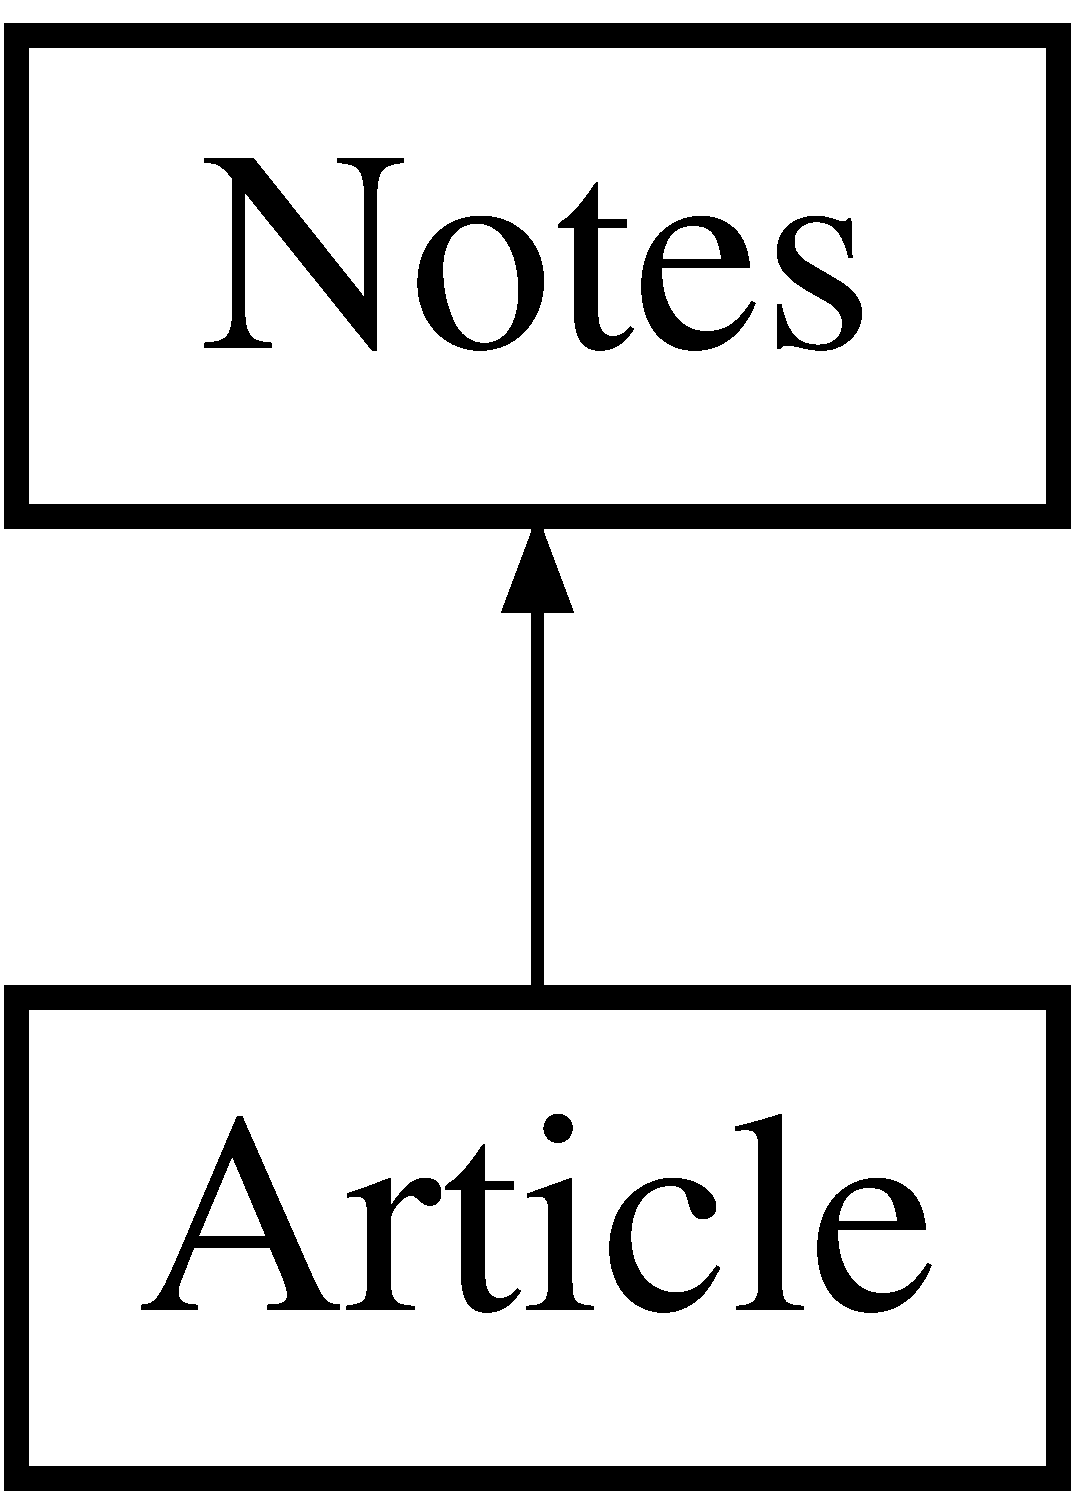
\includegraphics[height=2.000000cm]{class_article}
\end{center}
\end{figure}
\subsection*{Public Member Functions}
\begin{DoxyCompactItemize}
\item 
const Q\+String \& \hyperlink{class_article_a235fb07dfa8507b171c35624ada564d7}{get\+Text} () const
\begin{DoxyCompactList}\small\item\em get\+Text \end{DoxyCompactList}\item 
void \hyperlink{class_article_aae6c63348c0afa4422ed67afe55b8212}{set\+Texte} (const Q\+String \&s)
\begin{DoxyCompactList}\small\item\em set\+Texte \end{DoxyCompactList}\item 
\hyperlink{class_article_a4c6182f27ba97d7fe2031f1b675dd4a7}{Article} (const Q\+String i, const Q\+String titr, const Q\+String text)
\begin{DoxyCompactList}\small\item\em \hyperlink{class_article}{Article}. \end{DoxyCompactList}\item 
\hyperlink{class_article_a95de3a0b2d11ffe9c0bbf522dbc64c22}{Article} (const Q\+String i, const Q\+String titr, const Q\+String text, Q\+Date date\+Crea, Q\+Date date\+Modif)
\begin{DoxyCompactList}\small\item\em \hyperlink{class_article}{Article}. \end{DoxyCompactList}\item 
\mbox{\Hypertarget{class_article_a9db30863c1ede5d4c95e93625b620eea}\label{class_article_a9db30863c1ede5d4c95e93625b620eea}} 
void \hyperlink{class_article_a9db30863c1ede5d4c95e93625b620eea}{afficher} ()
\begin{DoxyCompactList}\small\item\em afficher \end{DoxyCompactList}\end{DoxyCompactItemize}


\subsection{Detailed Description}
The \hyperlink{class_article}{Article} class. 

\subsection{Constructor \& Destructor Documentation}
\mbox{\Hypertarget{class_article_a4c6182f27ba97d7fe2031f1b675dd4a7}\label{class_article_a4c6182f27ba97d7fe2031f1b675dd4a7}} 
\index{Article@{Article}!Article@{Article}}
\index{Article@{Article}!Article@{Article}}
\subsubsection{\texorpdfstring{Article()}{Article()}\hspace{0.1cm}{\footnotesize\ttfamily [1/2]}}
{\footnotesize\ttfamily Article\+::\+Article (\begin{DoxyParamCaption}\item[{const Q\+String}]{i,  }\item[{const Q\+String}]{titr,  }\item[{const Q\+String}]{text }\end{DoxyParamCaption})\hspace{0.3cm}{\ttfamily [inline]}}



\hyperlink{class_article}{Article}. 


\begin{DoxyParams}{Parameters}
{\em i} & \\
\hline
{\em titr} & \\
\hline
{\em text} & constructeur \\
\hline
\end{DoxyParams}
\mbox{\Hypertarget{class_article_a95de3a0b2d11ffe9c0bbf522dbc64c22}\label{class_article_a95de3a0b2d11ffe9c0bbf522dbc64c22}} 
\index{Article@{Article}!Article@{Article}}
\index{Article@{Article}!Article@{Article}}
\subsubsection{\texorpdfstring{Article()}{Article()}\hspace{0.1cm}{\footnotesize\ttfamily [2/2]}}
{\footnotesize\ttfamily Article\+::\+Article (\begin{DoxyParamCaption}\item[{const Q\+String}]{i,  }\item[{const Q\+String}]{titr,  }\item[{const Q\+String}]{text,  }\item[{Q\+Date}]{date\+Crea,  }\item[{Q\+Date}]{date\+Modif }\end{DoxyParamCaption})\hspace{0.3cm}{\ttfamily [inline]}}



\hyperlink{class_article}{Article}. 


\begin{DoxyParams}{Parameters}
{\em i} & \\
\hline
{\em titr} & \\
\hline
{\em text} & \\
\hline
{\em date\+Crea} & \\
\hline
{\em date\+Modif} & surcharge constructeur pour load \\
\hline
\end{DoxyParams}


\subsection{Member Function Documentation}
\mbox{\Hypertarget{class_article_a235fb07dfa8507b171c35624ada564d7}\label{class_article_a235fb07dfa8507b171c35624ada564d7}} 
\index{Article@{Article}!get\+Text@{get\+Text}}
\index{get\+Text@{get\+Text}!Article@{Article}}
\subsubsection{\texorpdfstring{get\+Text()}{getText()}}
{\footnotesize\ttfamily const Q\+String\& Article\+::get\+Text (\begin{DoxyParamCaption}{ }\end{DoxyParamCaption}) const\hspace{0.3cm}{\ttfamily [inline]}}



get\+Text 

\begin{DoxyReturn}{Returns}
texte de l\textquotesingle{}article 
\end{DoxyReturn}
\mbox{\Hypertarget{class_article_aae6c63348c0afa4422ed67afe55b8212}\label{class_article_aae6c63348c0afa4422ed67afe55b8212}} 
\index{Article@{Article}!set\+Texte@{set\+Texte}}
\index{set\+Texte@{set\+Texte}!Article@{Article}}
\subsubsection{\texorpdfstring{set\+Texte()}{setTexte()}}
{\footnotesize\ttfamily void Article\+::set\+Texte (\begin{DoxyParamCaption}\item[{const Q\+String \&}]{s }\end{DoxyParamCaption})\hspace{0.3cm}{\ttfamily [inline]}}



set\+Texte 


\begin{DoxyParams}{Parameters}
{\em s} & \\
\hline
\end{DoxyParams}


The documentation for this class was generated from the following files\+:\begin{DoxyCompactItemize}
\item 
notes.\+h\item 
notes.\+cpp\end{DoxyCompactItemize}

\hypertarget{class_article_editeur}{}\section{Article\+Editeur Class Reference}
\label{class_article_editeur}\index{Article\+Editeur@{Article\+Editeur}}


The \hyperlink{class_article_editeur}{Article\+Editeur} class permet afficher \hyperlink{class_article}{Article}, herite de \hyperlink{class_note_editeur}{Note\+Editeur}.  




{\ttfamily \#include $<$noteediteur.\+h$>$}

Inheritance diagram for Article\+Editeur\+:\begin{figure}[H]
\begin{center}
\leavevmode
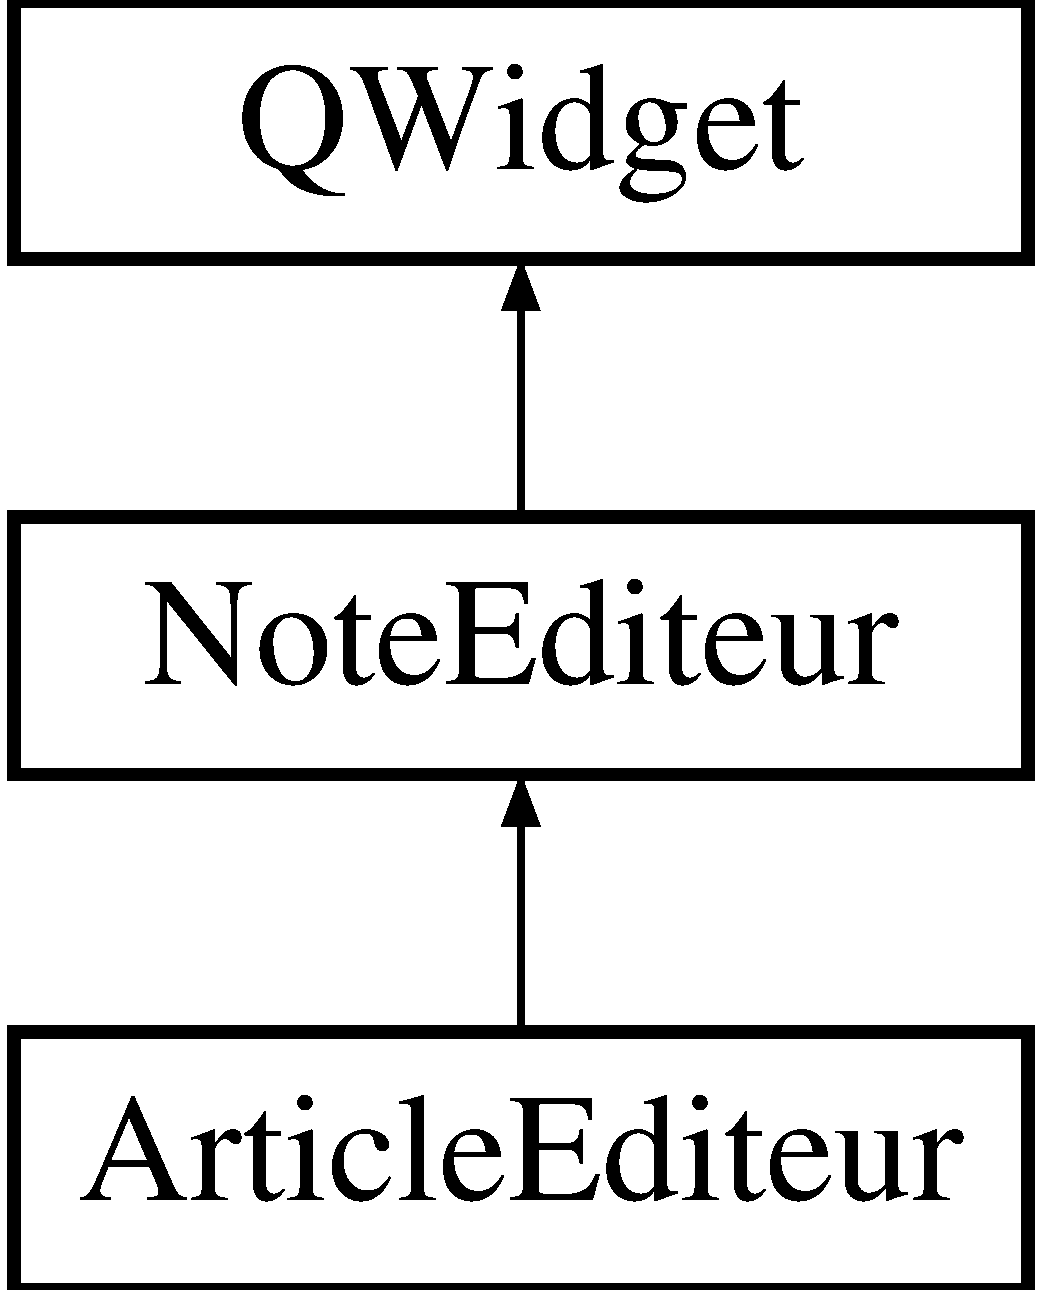
\includegraphics[height=3.000000cm]{class_article_editeur}
\end{center}
\end{figure}
\subsection*{Public Slots}
\begin{DoxyCompactItemize}
\item 
\mbox{\Hypertarget{class_article_editeur_a092cbfb381018789aa15cdfa1b31b63e}\label{class_article_editeur_a092cbfb381018789aa15cdfa1b31b63e}} 
void \hyperlink{class_article_editeur_a092cbfb381018789aa15cdfa1b31b63e}{save\+Article} ()
\begin{DoxyCompactList}\small\item\em save\+Article enregistrer modif article \end{DoxyCompactList}\item 
\mbox{\Hypertarget{class_article_editeur_aba5870b0dac1d6da7a3e585547038e09}\label{class_article_editeur_aba5870b0dac1d6da7a3e585547038e09}} 
void \hyperlink{class_article_editeur_aba5870b0dac1d6da7a3e585547038e09}{archiver\+Article} ()
\begin{DoxyCompactList}\small\item\em archiver\+Article archiver un article \end{DoxyCompactList}\item 
\mbox{\Hypertarget{class_article_editeur_a91d3782a6afb9e6b769a319fb5c42a4c}\label{class_article_editeur_a91d3782a6afb9e6b769a319fb5c42a4c}} 
void \hyperlink{class_article_editeur_a91d3782a6afb9e6b769a319fb5c42a4c}{restaurer\+Article} ()
\begin{DoxyCompactList}\small\item\em restaurer\+Article restaurer un article \end{DoxyCompactList}\end{DoxyCompactItemize}
\subsection*{Public Member Functions}
\begin{DoxyCompactItemize}
\item 
\hyperlink{class_article_editeur_a5dd5b7ad1e2076e432deeb40817c4b19}{Article\+Editeur} (\hyperlink{class_article}{Article} \&art, \hyperlink{class_fenetre_principale}{Fenetre\+Principale} $\ast$p)
\begin{DoxyCompactList}\small\item\em \hyperlink{class_article_editeur}{Article\+Editeur}. \end{DoxyCompactList}\item 
\hyperlink{class_article_editeur_ad83c4235eddf80bcd2be5bd80d49a06a}{Article\+Editeur} (\hyperlink{class_article}{Article} \&art, \hyperlink{class_fenetre_principale}{Fenetre\+Principale} $\ast$p, int j)
\begin{DoxyCompactList}\small\item\em \hyperlink{class_article_editeur}{Article\+Editeur}. \end{DoxyCompactList}\end{DoxyCompactItemize}


\subsection{Detailed Description}
The \hyperlink{class_article_editeur}{Article\+Editeur} class permet afficher \hyperlink{class_article}{Article}, herite de \hyperlink{class_note_editeur}{Note\+Editeur}. 

\subsection{Constructor \& Destructor Documentation}
\mbox{\Hypertarget{class_article_editeur_a5dd5b7ad1e2076e432deeb40817c4b19}\label{class_article_editeur_a5dd5b7ad1e2076e432deeb40817c4b19}} 
\index{Article\+Editeur@{Article\+Editeur}!Article\+Editeur@{Article\+Editeur}}
\index{Article\+Editeur@{Article\+Editeur}!Article\+Editeur@{Article\+Editeur}}
\subsubsection{\texorpdfstring{Article\+Editeur()}{ArticleEditeur()}\hspace{0.1cm}{\footnotesize\ttfamily [1/2]}}
{\footnotesize\ttfamily Article\+Editeur\+::\+Article\+Editeur (\begin{DoxyParamCaption}\item[{\hyperlink{class_article}{Article} \&}]{art,  }\item[{\hyperlink{class_fenetre_principale}{Fenetre\+Principale} $\ast$}]{p }\end{DoxyParamCaption})}



\hyperlink{class_article_editeur}{Article\+Editeur}. 


\begin{DoxyParams}{Parameters}
{\em art} & article à afficher \\
\hline
{\em p} & \hyperlink{class_fenetre_principale}{Fenetre\+Principale} dans laquelle afficher \\
\hline
\end{DoxyParams}
\mbox{\Hypertarget{class_article_editeur_ad83c4235eddf80bcd2be5bd80d49a06a}\label{class_article_editeur_ad83c4235eddf80bcd2be5bd80d49a06a}} 
\index{Article\+Editeur@{Article\+Editeur}!Article\+Editeur@{Article\+Editeur}}
\index{Article\+Editeur@{Article\+Editeur}!Article\+Editeur@{Article\+Editeur}}
\subsubsection{\texorpdfstring{Article\+Editeur()}{ArticleEditeur()}\hspace{0.1cm}{\footnotesize\ttfamily [2/2]}}
{\footnotesize\ttfamily Article\+Editeur\+::\+Article\+Editeur (\begin{DoxyParamCaption}\item[{\hyperlink{class_article}{Article} \&}]{art,  }\item[{\hyperlink{class_fenetre_principale}{Fenetre\+Principale} $\ast$}]{p,  }\item[{int}]{j }\end{DoxyParamCaption})}



\hyperlink{class_article_editeur}{Article\+Editeur}. 


\begin{DoxyParams}{Parameters}
{\em art} & article à afficher \\
\hline
{\em p} & \hyperlink{class_fenetre_principale}{Fenetre\+Principale} dans laquelle afficher \\
\hline
{\em j} & pour savoir si archive ou pas \\
\hline
\end{DoxyParams}


The documentation for this class was generated from the following files\+:\begin{DoxyCompactItemize}
\item 
noteediteur.\+h\item 
noteediteur.\+cpp\end{DoxyCompactItemize}

\hypertarget{class_couple}{}\section{Couple Class Reference}
\label{class_couple}\index{Couple@{Couple}}


The \hyperlink{class_couple}{Couple} class contient un couple de 2 notes.  




{\ttfamily \#include $<$relation.\+h$>$}

\subsection*{Public Member Functions}
\begin{DoxyCompactItemize}
\item 
\hyperlink{class_couple_abe99267749e9b76abe4401c1f888f354}{Couple} (\hyperlink{class_notes}{Notes} \&a, \hyperlink{class_notes}{Notes} \&b, Q\+String l=\char`\"{}\char`\"{})
\begin{DoxyCompactList}\small\item\em \hyperlink{class_couple}{Couple}. \end{DoxyCompactList}\item 
\hyperlink{class_notes}{Notes} \& \hyperlink{class_couple_acd88fe5ee43929a72a95c6c5129e6fbd}{get\+Note1} () const
\begin{DoxyCompactList}\small\item\em get\+Note1 \end{DoxyCompactList}\item 
\hyperlink{class_notes}{Notes} \& \hyperlink{class_couple_a8e9f87f1c450bf8c21514a04b7734c45}{get\+Note2} () const
\begin{DoxyCompactList}\small\item\em get\+Note2 \end{DoxyCompactList}\item 
const Q\+String \& \hyperlink{class_couple_a0f04e0130d4d44ce39e322033d85a8df}{get\+Label} () const
\begin{DoxyCompactList}\small\item\em get\+Label \end{DoxyCompactList}\item 
void \hyperlink{class_couple_aa2369d7e4e139a7dcba583b4688536bf}{set\+Label} (const Q\+String \&newL)
\begin{DoxyCompactList}\small\item\em set\+Label \end{DoxyCompactList}\item 
bool \hyperlink{class_couple_a493af8c8763ceef4cadf82787a3ccf47}{operator==} (const \hyperlink{class_couple}{Couple} \&c)
\begin{DoxyCompactList}\small\item\em operator == \end{DoxyCompactList}\end{DoxyCompactItemize}


\subsection{Detailed Description}
The \hyperlink{class_couple}{Couple} class contient un couple de 2 notes. 

\subsection{Constructor \& Destructor Documentation}
\mbox{\Hypertarget{class_couple_abe99267749e9b76abe4401c1f888f354}\label{class_couple_abe99267749e9b76abe4401c1f888f354}} 
\index{Couple@{Couple}!Couple@{Couple}}
\index{Couple@{Couple}!Couple@{Couple}}
\subsubsection{\texorpdfstring{Couple()}{Couple()}}
{\footnotesize\ttfamily Couple\+::\+Couple (\begin{DoxyParamCaption}\item[{\hyperlink{class_notes}{Notes} \&}]{a,  }\item[{\hyperlink{class_notes}{Notes} \&}]{b,  }\item[{Q\+String}]{l = {\ttfamily \char`\"{}\char`\"{}} }\end{DoxyParamCaption})\hspace{0.3cm}{\ttfamily [inline]}}



\hyperlink{class_couple}{Couple}. 


\begin{DoxyParams}{Parameters}
{\em a} & \\
\hline
{\em b} & \\
\hline
{\em l} & \\
\hline
\end{DoxyParams}


\subsection{Member Function Documentation}
\mbox{\Hypertarget{class_couple_a0f04e0130d4d44ce39e322033d85a8df}\label{class_couple_a0f04e0130d4d44ce39e322033d85a8df}} 
\index{Couple@{Couple}!get\+Label@{get\+Label}}
\index{get\+Label@{get\+Label}!Couple@{Couple}}
\subsubsection{\texorpdfstring{get\+Label()}{getLabel()}}
{\footnotesize\ttfamily const Q\+String\& Couple\+::get\+Label (\begin{DoxyParamCaption}{ }\end{DoxyParamCaption}) const\hspace{0.3cm}{\ttfamily [inline]}}



get\+Label 

\begin{DoxyReturn}{Returns}
le label 
\end{DoxyReturn}
\mbox{\Hypertarget{class_couple_acd88fe5ee43929a72a95c6c5129e6fbd}\label{class_couple_acd88fe5ee43929a72a95c6c5129e6fbd}} 
\index{Couple@{Couple}!get\+Note1@{get\+Note1}}
\index{get\+Note1@{get\+Note1}!Couple@{Couple}}
\subsubsection{\texorpdfstring{get\+Note1()}{getNote1()}}
{\footnotesize\ttfamily \hyperlink{class_notes}{Notes}\& Couple\+::get\+Note1 (\begin{DoxyParamCaption}{ }\end{DoxyParamCaption}) const\hspace{0.3cm}{\ttfamily [inline]}}



get\+Note1 

\begin{DoxyReturn}{Returns}
la premiere note 
\end{DoxyReturn}
\mbox{\Hypertarget{class_couple_a8e9f87f1c450bf8c21514a04b7734c45}\label{class_couple_a8e9f87f1c450bf8c21514a04b7734c45}} 
\index{Couple@{Couple}!get\+Note2@{get\+Note2}}
\index{get\+Note2@{get\+Note2}!Couple@{Couple}}
\subsubsection{\texorpdfstring{get\+Note2()}{getNote2()}}
{\footnotesize\ttfamily \hyperlink{class_notes}{Notes}\& Couple\+::get\+Note2 (\begin{DoxyParamCaption}{ }\end{DoxyParamCaption}) const\hspace{0.3cm}{\ttfamily [inline]}}



get\+Note2 

\begin{DoxyReturn}{Returns}
la deuxieme note 
\end{DoxyReturn}
\mbox{\Hypertarget{class_couple_a493af8c8763ceef4cadf82787a3ccf47}\label{class_couple_a493af8c8763ceef4cadf82787a3ccf47}} 
\index{Couple@{Couple}!operator==@{operator==}}
\index{operator==@{operator==}!Couple@{Couple}}
\subsubsection{\texorpdfstring{operator==()}{operator==()}}
{\footnotesize\ttfamily bool Couple\+::operator== (\begin{DoxyParamCaption}\item[{const \hyperlink{class_couple}{Couple} \&}]{c }\end{DoxyParamCaption})}



operator == 


\begin{DoxyParams}{Parameters}
{\em c} & \\
\hline
\end{DoxyParams}
\begin{DoxyReturn}{Returns}
bool surcharge operateur == 
\end{DoxyReturn}
\mbox{\Hypertarget{class_couple_aa2369d7e4e139a7dcba583b4688536bf}\label{class_couple_aa2369d7e4e139a7dcba583b4688536bf}} 
\index{Couple@{Couple}!set\+Label@{set\+Label}}
\index{set\+Label@{set\+Label}!Couple@{Couple}}
\subsubsection{\texorpdfstring{set\+Label()}{setLabel()}}
{\footnotesize\ttfamily void Couple\+::set\+Label (\begin{DoxyParamCaption}\item[{const Q\+String \&}]{newL }\end{DoxyParamCaption})\hspace{0.3cm}{\ttfamily [inline]}}



set\+Label 


\begin{DoxyParams}{Parameters}
{\em newL} & accesseur en ecriture \\
\hline
\end{DoxyParams}


The documentation for this class was generated from the following files\+:\begin{DoxyCompactItemize}
\item 
relation.\+h\item 
relation.\+cpp\end{DoxyCompactItemize}

\hypertarget{class_fenetre_creer_article}{}\section{Fenetre\+Creer\+Article Class Reference}
\label{class_fenetre_creer_article}\index{Fenetre\+Creer\+Article@{Fenetre\+Creer\+Article}}


The \hyperlink{class_fenetre_creer_article}{Fenetre\+Creer\+Article} class fenetre pour créer un article.  




{\ttfamily \#include $<$fenetrecreerarticle.\+h$>$}

Inheritance diagram for Fenetre\+Creer\+Article\+:\begin{figure}[H]
\begin{center}
\leavevmode
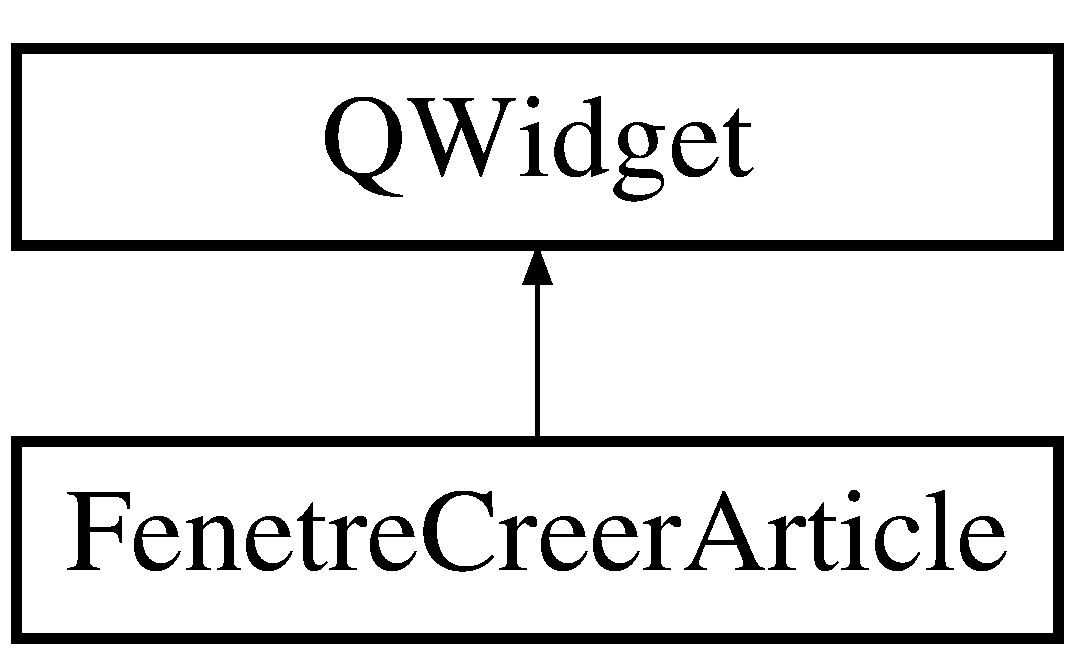
\includegraphics[height=2.000000cm]{class_fenetre_creer_article}
\end{center}
\end{figure}
\subsection*{Public Slots}
\begin{DoxyCompactItemize}
\item 
\mbox{\Hypertarget{class_fenetre_creer_article_a1af9df05c8281484ded9773948c08eaa}\label{class_fenetre_creer_article_a1af9df05c8281484ded9773948c08eaa}} 
void \hyperlink{class_fenetre_creer_article_a1af9df05c8281484ded9773948c08eaa}{ajouter\+Article} ()
\begin{DoxyCompactList}\small\item\em ajouter\+Article gère insertion dans Histo\+Notes\+Manager \end{DoxyCompactList}\end{DoxyCompactItemize}
\subsection*{Public Member Functions}
\begin{DoxyCompactItemize}
\item 
\hyperlink{class_fenetre_creer_article_a42dc0e10146b018c2c77ceb9a6fda815}{Fenetre\+Creer\+Article} (\hyperlink{class_fenetre_principale}{Fenetre\+Principale} $\ast$p)
\begin{DoxyCompactList}\small\item\em \hyperlink{class_fenetre_creer_article}{Fenetre\+Creer\+Article}. \end{DoxyCompactList}\end{DoxyCompactItemize}


\subsection{Detailed Description}
The \hyperlink{class_fenetre_creer_article}{Fenetre\+Creer\+Article} class fenetre pour créer un article. 

\subsection{Constructor \& Destructor Documentation}
\mbox{\Hypertarget{class_fenetre_creer_article_a42dc0e10146b018c2c77ceb9a6fda815}\label{class_fenetre_creer_article_a42dc0e10146b018c2c77ceb9a6fda815}} 
\index{Fenetre\+Creer\+Article@{Fenetre\+Creer\+Article}!Fenetre\+Creer\+Article@{Fenetre\+Creer\+Article}}
\index{Fenetre\+Creer\+Article@{Fenetre\+Creer\+Article}!Fenetre\+Creer\+Article@{Fenetre\+Creer\+Article}}
\subsubsection{\texorpdfstring{Fenetre\+Creer\+Article()}{FenetreCreerArticle()}}
{\footnotesize\ttfamily Fenetre\+Creer\+Article\+::\+Fenetre\+Creer\+Article (\begin{DoxyParamCaption}\item[{\hyperlink{class_fenetre_principale}{Fenetre\+Principale} $\ast$}]{p }\end{DoxyParamCaption})}



\hyperlink{class_fenetre_creer_article}{Fenetre\+Creer\+Article}. 


\begin{DoxyParams}{Parameters}
{\em p} & fenetre principale \\
\hline
\end{DoxyParams}


The documentation for this class was generated from the following files\+:\begin{DoxyCompactItemize}
\item 
fenetrecreerarticle.\+h\item 
fenetrecreerarticle.\+cpp\end{DoxyCompactItemize}

\hypertarget{class_fenetre_creer_multi}{}\section{Fenetre\+Creer\+Multi Class Reference}
\label{class_fenetre_creer_multi}\index{Fenetre\+Creer\+Multi@{Fenetre\+Creer\+Multi}}


The \hyperlink{class_fenetre_creer_multi}{Fenetre\+Creer\+Multi} class fenetre pour creer un multimedia.  




{\ttfamily \#include $<$Fenetre\+Creer\+Multi.\+h$>$}

Inheritance diagram for Fenetre\+Creer\+Multi\+:\begin{figure}[H]
\begin{center}
\leavevmode
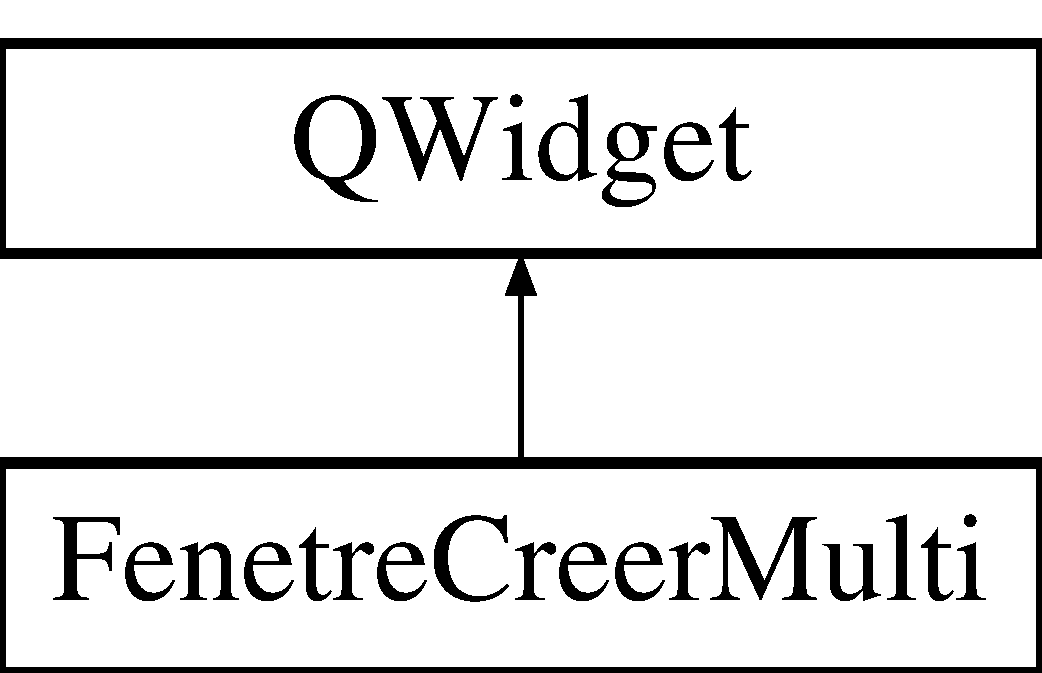
\includegraphics[height=2.000000cm]{class_fenetre_creer_multi}
\end{center}
\end{figure}
\subsection*{Public Slots}
\begin{DoxyCompactItemize}
\item 
\mbox{\Hypertarget{class_fenetre_creer_multi_a70f6413728fbd559a306c9af4f2c1e5f}\label{class_fenetre_creer_multi_a70f6413728fbd559a306c9af4f2c1e5f}} 
void \hyperlink{class_fenetre_creer_multi_a70f6413728fbd559a306c9af4f2c1e5f}{ajouter\+Multi} ()
\begin{DoxyCompactList}\small\item\em ajouter\+Multi gere insertion du multimedia dans \hyperlink{class_histo_note_manager}{Histo\+Note\+Manager} \end{DoxyCompactList}\end{DoxyCompactItemize}
\subsection*{Public Member Functions}
\begin{DoxyCompactItemize}
\item 
\hyperlink{class_fenetre_creer_multi_a231eaaeeeae9cccd5bab64515a6eeab8}{Fenetre\+Creer\+Multi} (\hyperlink{class_fenetre_principale}{Fenetre\+Principale} $\ast$p)
\begin{DoxyCompactList}\small\item\em \hyperlink{class_fenetre_creer_multi}{Fenetre\+Creer\+Multi}. \end{DoxyCompactList}\end{DoxyCompactItemize}


\subsection{Detailed Description}
The \hyperlink{class_fenetre_creer_multi}{Fenetre\+Creer\+Multi} class fenetre pour creer un multimedia. 

\subsection{Constructor \& Destructor Documentation}
\mbox{\Hypertarget{class_fenetre_creer_multi_a231eaaeeeae9cccd5bab64515a6eeab8}\label{class_fenetre_creer_multi_a231eaaeeeae9cccd5bab64515a6eeab8}} 
\index{Fenetre\+Creer\+Multi@{Fenetre\+Creer\+Multi}!Fenetre\+Creer\+Multi@{Fenetre\+Creer\+Multi}}
\index{Fenetre\+Creer\+Multi@{Fenetre\+Creer\+Multi}!Fenetre\+Creer\+Multi@{Fenetre\+Creer\+Multi}}
\subsubsection{\texorpdfstring{Fenetre\+Creer\+Multi()}{FenetreCreerMulti()}}
{\footnotesize\ttfamily Fenetre\+Creer\+Multi\+::\+Fenetre\+Creer\+Multi (\begin{DoxyParamCaption}\item[{\hyperlink{class_fenetre_principale}{Fenetre\+Principale} $\ast$}]{p }\end{DoxyParamCaption})}



\hyperlink{class_fenetre_creer_multi}{Fenetre\+Creer\+Multi}. 


\begin{DoxyParams}{Parameters}
{\em p} & \\
\hline
\end{DoxyParams}


The documentation for this class was generated from the following files\+:\begin{DoxyCompactItemize}
\item 
Fenetre\+Creer\+Multi.\+h\item 
Fenetre\+Creer\+Multi.\+cpp\end{DoxyCompactItemize}

\hypertarget{class_fenetre_creer_relation}{}\section{Fenetre\+Creer\+Relation Class Reference}
\label{class_fenetre_creer_relation}\index{Fenetre\+Creer\+Relation@{Fenetre\+Creer\+Relation}}


The \hyperlink{class_fenetre_creer_relation}{Fenetre\+Creer\+Relation} class fenetre pour creer une relation.  




{\ttfamily \#include $<$Fenetre\+Creer\+Relation.\+h$>$}

Inheritance diagram for Fenetre\+Creer\+Relation\+:\begin{figure}[H]
\begin{center}
\leavevmode
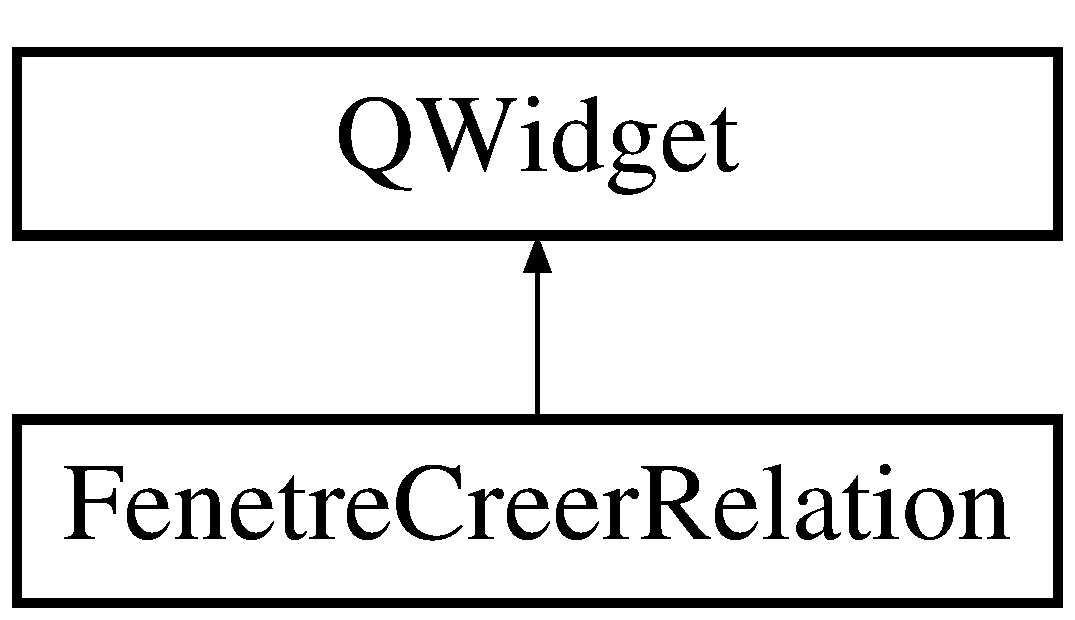
\includegraphics[height=2.000000cm]{class_fenetre_creer_relation}
\end{center}
\end{figure}
\subsection*{Public Slots}
\begin{DoxyCompactItemize}
\item 
\mbox{\Hypertarget{class_fenetre_creer_relation_a675a698684b3199f49ac3e51b34c9b30}\label{class_fenetre_creer_relation_a675a698684b3199f49ac3e51b34c9b30}} 
void \hyperlink{class_fenetre_creer_relation_a675a698684b3199f49ac3e51b34c9b30}{ajouter\+Relation} ()
\begin{DoxyCompactList}\small\item\em ajouter\+Relation gere insertion dans \hyperlink{class_histo_note_manager}{Histo\+Note\+Manager} \end{DoxyCompactList}\end{DoxyCompactItemize}
\subsection*{Public Member Functions}
\begin{DoxyCompactItemize}
\item 
\hyperlink{class_fenetre_creer_relation_ae9f3e3635ed7130fa00c215a1d0454ec}{Fenetre\+Creer\+Relation} (\hyperlink{class_fenetre_principale}{Fenetre\+Principale} $\ast$p)
\begin{DoxyCompactList}\small\item\em \hyperlink{class_fenetre_creer_relation}{Fenetre\+Creer\+Relation}. \end{DoxyCompactList}\end{DoxyCompactItemize}


\subsection{Detailed Description}
The \hyperlink{class_fenetre_creer_relation}{Fenetre\+Creer\+Relation} class fenetre pour creer une relation. 

\subsection{Constructor \& Destructor Documentation}
\mbox{\Hypertarget{class_fenetre_creer_relation_ae9f3e3635ed7130fa00c215a1d0454ec}\label{class_fenetre_creer_relation_ae9f3e3635ed7130fa00c215a1d0454ec}} 
\index{Fenetre\+Creer\+Relation@{Fenetre\+Creer\+Relation}!Fenetre\+Creer\+Relation@{Fenetre\+Creer\+Relation}}
\index{Fenetre\+Creer\+Relation@{Fenetre\+Creer\+Relation}!Fenetre\+Creer\+Relation@{Fenetre\+Creer\+Relation}}
\subsubsection{\texorpdfstring{Fenetre\+Creer\+Relation()}{FenetreCreerRelation()}}
{\footnotesize\ttfamily Fenetre\+Creer\+Relation\+::\+Fenetre\+Creer\+Relation (\begin{DoxyParamCaption}\item[{\hyperlink{class_fenetre_principale}{Fenetre\+Principale} $\ast$}]{p }\end{DoxyParamCaption})}



\hyperlink{class_fenetre_creer_relation}{Fenetre\+Creer\+Relation}. 


\begin{DoxyParams}{Parameters}
{\em p} & \\
\hline
\end{DoxyParams}


The documentation for this class was generated from the following files\+:\begin{DoxyCompactItemize}
\item 
Fenetre\+Creer\+Relation.\+h\item 
Fenetre\+Creer\+Relation.\+cpp\end{DoxyCompactItemize}

\hypertarget{class_fenetre_creer_tache}{}\section{Fenetre\+Creer\+Tache Class Reference}
\label{class_fenetre_creer_tache}\index{Fenetre\+Creer\+Tache@{Fenetre\+Creer\+Tache}}


The \hyperlink{class_fenetre_creer_tache}{Fenetre\+Creer\+Tache} class fenetre pour creer une tache.  




{\ttfamily \#include $<$fenetrecreertache.\+h$>$}

Inheritance diagram for Fenetre\+Creer\+Tache\+:\begin{figure}[H]
\begin{center}
\leavevmode
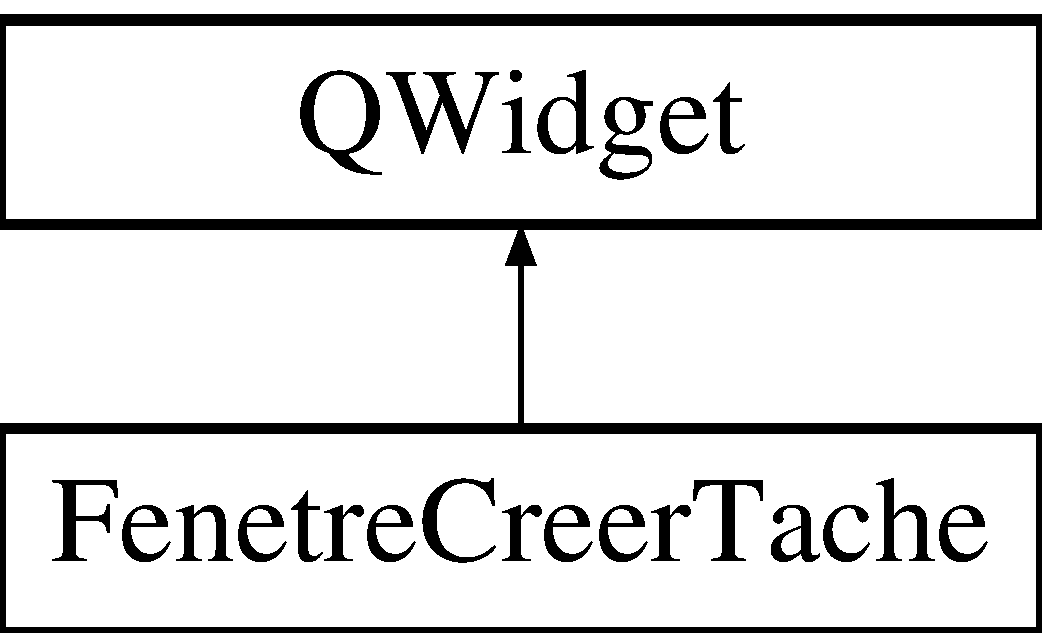
\includegraphics[height=2.000000cm]{class_fenetre_creer_tache}
\end{center}
\end{figure}
\subsection*{Public Slots}
\begin{DoxyCompactItemize}
\item 
\mbox{\Hypertarget{class_fenetre_creer_tache_aedd811e90cb80f2f8c8509b313884be0}\label{class_fenetre_creer_tache_aedd811e90cb80f2f8c8509b313884be0}} 
void \hyperlink{class_fenetre_creer_tache_aedd811e90cb80f2f8c8509b313884be0}{ajouter\+Tache} ()
\begin{DoxyCompactList}\small\item\em ajouter\+Tache gere insertion tache dans \hyperlink{class_histo_note_manager}{Histo\+Note\+Manager} \end{DoxyCompactList}\end{DoxyCompactItemize}
\subsection*{Public Member Functions}
\begin{DoxyCompactItemize}
\item 
\mbox{\Hypertarget{class_fenetre_creer_tache_ac1c51570b4c20c80fb9be43c8ce708b0}\label{class_fenetre_creer_tache_ac1c51570b4c20c80fb9be43c8ce708b0}} 
{\bfseries Fenetre\+Creer\+Tache} (\hyperlink{class_fenetre_principale}{Fenetre\+Principale} $\ast$p)
\end{DoxyCompactItemize}


\subsection{Detailed Description}
The \hyperlink{class_fenetre_creer_tache}{Fenetre\+Creer\+Tache} class fenetre pour creer une tache. 

The documentation for this class was generated from the following files\+:\begin{DoxyCompactItemize}
\item 
fenetrecreertache.\+h\item 
fenetrecreertache.\+cpp\end{DoxyCompactItemize}

\hypertarget{class_fenetre_principale}{}\section{Fenetre\+Principale Class Reference}
\label{class_fenetre_principale}\index{Fenetre\+Principale@{Fenetre\+Principale}}


The \hyperlink{class_fenetre_principale}{Fenetre\+Principale} class.  




{\ttfamily \#include $<$fenprincipale.\+h$>$}

Inheritance diagram for Fenetre\+Principale\+:\begin{figure}[H]
\begin{center}
\leavevmode
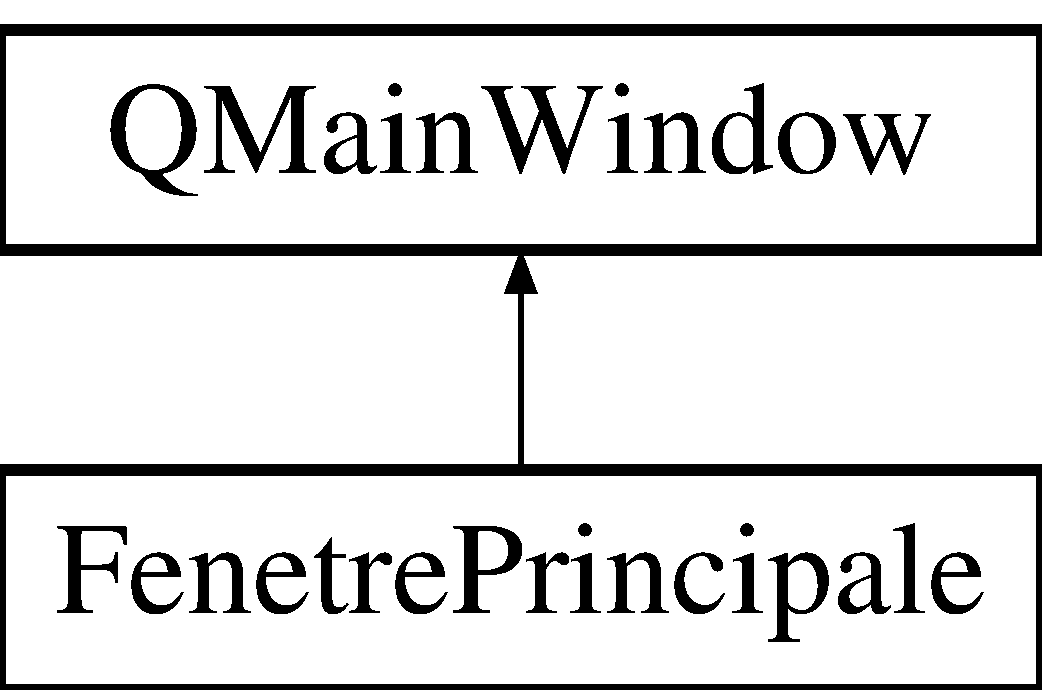
\includegraphics[height=2.000000cm]{class_fenetre_principale}
\end{center}
\end{figure}
\subsection*{Public Slots}
\begin{DoxyCompactItemize}
\item 
\mbox{\Hypertarget{class_fenetre_principale_a8ccbf1f04c52130f106ff14ec427709f}\label{class_fenetre_principale_a8ccbf1f04c52130f106ff14ec427709f}} 
void \hyperlink{class_fenetre_principale_a8ccbf1f04c52130f106ff14ec427709f}{afficher\+Creer\+Article} ()
\begin{DoxyCompactList}\small\item\em afficher\+Creer\+Article ouvre fenetre pour creer un article \end{DoxyCompactList}\item 
\mbox{\Hypertarget{class_fenetre_principale_af572d9ec04d80f65bd8dd27616d2ea1f}\label{class_fenetre_principale_af572d9ec04d80f65bd8dd27616d2ea1f}} 
void \hyperlink{class_fenetre_principale_af572d9ec04d80f65bd8dd27616d2ea1f}{afficher\+Creer\+Tache} ()
\begin{DoxyCompactList}\small\item\em afficher\+Creer\+Tache ouvre fenetre pour creer un tache \end{DoxyCompactList}\item 
\mbox{\Hypertarget{class_fenetre_principale_a0c1fbc3e1e5a8921d989a2d4c4116397}\label{class_fenetre_principale_a0c1fbc3e1e5a8921d989a2d4c4116397}} 
void \hyperlink{class_fenetre_principale_a0c1fbc3e1e5a8921d989a2d4c4116397}{afficher\+Creer\+Multi} ()
\begin{DoxyCompactList}\small\item\em afficher\+Creer\+Multi ouvre fenetre pour creer un multimedia \end{DoxyCompactList}\item 
\mbox{\Hypertarget{class_fenetre_principale_a154654b4aaf695be6445ff0d42c2669c}\label{class_fenetre_principale_a154654b4aaf695be6445ff0d42c2669c}} 
void \hyperlink{class_fenetre_principale_a154654b4aaf695be6445ff0d42c2669c}{afficher\+Creer\+Relation} ()
\begin{DoxyCompactList}\small\item\em afficher\+Creer\+Relation ouvre fenetre pour creer une relation \end{DoxyCompactList}\item 
\mbox{\Hypertarget{class_fenetre_principale_a78e23e66e42390fff9936f121f2b47b4}\label{class_fenetre_principale_a78e23e66e42390fff9936f121f2b47b4}} 
void \hyperlink{class_fenetre_principale_a78e23e66e42390fff9936f121f2b47b4}{afficher\+Article} ()
\begin{DoxyCompactList}\small\item\em afficher\+Article affiche article selectionné au milieu \end{DoxyCompactList}\item 
\mbox{\Hypertarget{class_fenetre_principale_a9295ee1fd8501a8dcc39f3bea03885fc}\label{class_fenetre_principale_a9295ee1fd8501a8dcc39f3bea03885fc}} 
void \hyperlink{class_fenetre_principale_a9295ee1fd8501a8dcc39f3bea03885fc}{afficher\+Tache} ()
\begin{DoxyCompactList}\small\item\em afficher\+Tache affiche tache selectionné au milieu \end{DoxyCompactList}\item 
\mbox{\Hypertarget{class_fenetre_principale_a1ee3cca5ac799105f4a30b4cbcb811ed}\label{class_fenetre_principale_a1ee3cca5ac799105f4a30b4cbcb811ed}} 
void \hyperlink{class_fenetre_principale_a1ee3cca5ac799105f4a30b4cbcb811ed}{afficher\+Multi} ()
\begin{DoxyCompactList}\small\item\em afficher\+Multi affiche multimedia selectionné au milieu \end{DoxyCompactList}\item 
\mbox{\Hypertarget{class_fenetre_principale_a63c50d1b25d15bd175baa8d7b357a10b}\label{class_fenetre_principale_a63c50d1b25d15bd175baa8d7b357a10b}} 
void \hyperlink{class_fenetre_principale_a63c50d1b25d15bd175baa8d7b357a10b}{afficher\+Archive} ()
\begin{DoxyCompactList}\small\item\em afficher\+Archive affiche archive selectionné au milieu \end{DoxyCompactList}\end{DoxyCompactItemize}
\subsection*{Public Member Functions}
\begin{DoxyCompactItemize}
\item 
\mbox{\Hypertarget{class_fenetre_principale_a1226b3f74369ed9d6e577b26d0db11fb}\label{class_fenetre_principale_a1226b3f74369ed9d6e577b26d0db11fb}} 
\hyperlink{class_fenetre_principale_a1226b3f74369ed9d6e577b26d0db11fb}{Fenetre\+Principale} ()
\begin{DoxyCompactList}\small\item\em \hyperlink{class_fenetre_principale}{Fenetre\+Principale}. \end{DoxyCompactList}\item 
\mbox{\Hypertarget{class_fenetre_principale_a7bbe4f01fce9c861569cc9a6c6cb6278}\label{class_fenetre_principale_a7bbe4f01fce9c861569cc9a6c6cb6278}} 
void \hyperlink{class_fenetre_principale_a7bbe4f01fce9c861569cc9a6c6cb6278}{update\+Articles} ()
\begin{DoxyCompactList}\small\item\em update\+Articles gere affichage liste article \end{DoxyCompactList}\item 
\mbox{\Hypertarget{class_fenetre_principale_a55114ce4cb1a940c917834d15fe811c7}\label{class_fenetre_principale_a55114ce4cb1a940c917834d15fe811c7}} 
void \hyperlink{class_fenetre_principale_a55114ce4cb1a940c917834d15fe811c7}{update\+Multi} ()
\begin{DoxyCompactList}\small\item\em update\+Multi gere affichage liste multi \end{DoxyCompactList}\item 
\mbox{\Hypertarget{class_fenetre_principale_a332356aa53313347d58fe5c68288f9d3}\label{class_fenetre_principale_a332356aa53313347d58fe5c68288f9d3}} 
void \hyperlink{class_fenetre_principale_a332356aa53313347d58fe5c68288f9d3}{update\+Taches} ()
\begin{DoxyCompactList}\small\item\em update\+Tache gere affichage liste tache \end{DoxyCompactList}\item 
\mbox{\Hypertarget{class_fenetre_principale_ad8e5e7ebc79b842fd75c59e666ed7255}\label{class_fenetre_principale_ad8e5e7ebc79b842fd75c59e666ed7255}} 
void \hyperlink{class_fenetre_principale_ad8e5e7ebc79b842fd75c59e666ed7255}{update\+Archives} ()
\begin{DoxyCompactList}\small\item\em update\+Archives gere affichage liste archive \end{DoxyCompactList}\item 
\mbox{\Hypertarget{class_fenetre_principale_aba9b6d1406b9b92cf649f170671740aa}\label{class_fenetre_principale_aba9b6d1406b9b92cf649f170671740aa}} 
void \hyperlink{class_fenetre_principale_aba9b6d1406b9b92cf649f170671740aa}{update\+Relation} ()
\begin{DoxyCompactList}\small\item\em update\+Relation gere affichage liste relation \end{DoxyCompactList}\end{DoxyCompactItemize}


\subsection{Detailed Description}
The \hyperlink{class_fenetre_principale}{Fenetre\+Principale} class. 

The documentation for this class was generated from the following files\+:\begin{DoxyCompactItemize}
\item 
fenprincipale.\+h\item 
fenprincipale.\+cpp\end{DoxyCompactItemize}

\hypertarget{class_histo_note_manager}{}\section{Histo\+Note\+Manager Class Reference}
\label{class_histo_note_manager}\index{Histo\+Note\+Manager@{Histo\+Note\+Manager}}


The \hyperlink{class_histo_note_manager}{Histo\+Note\+Manager} class \hyperlink{class_histo_note_manager}{Histo\+Note\+Manager} est la classe principale de l\textquotesingle{}application \+: il n\textquotesingle{}existe qu\textquotesingle{}une seule instance de cette classe ( design pattern singleton). Cette classe permet de manipuler les différents \hyperlink{class_histo_notes}{Histo\+Notes} ( \hyperlink{class_article}{Article}, \hyperlink{class_tache}{Tache}, Mutimedia ) à l\textquotesingle{}aide de 3 attributs ( de type double pointeur sur \hyperlink{class_histo_notes}{Histo\+Notes}) \+: articles, taches, multimedias. \hyperlink{class_histo_note_manager}{Histo\+Note\+Manager} est le point de départ de toutes créations \+: c\textquotesingle{}est elle qui permet la creation des \hyperlink{class_histo_notes}{Histo\+Notes}, et donc des \hyperlink{class_notes}{Notes}.  




{\ttfamily \#include $<$histonotes.\+h$>$}

\subsection*{Classes}
\begin{DoxyCompactItemize}
\item 
class \hyperlink{class_histo_note_manager_1_1iterator}{iterator}
\begin{DoxyCompactList}\small\item\em The iterator class Classe permettant de parcourir tous les tableaux de pointeur de \hyperlink{class_histo_note_manager}{Histo\+Note\+Manager} sans que la structure des données utilisée soit revelée Pour cela nous avons surcharger plusieurs operateurs et créer des fonctions permettant d\textquotesingle{}accéder au début ou à la fin de la structure de donnée. \end{DoxyCompactList}\end{DoxyCompactItemize}
\subsection*{Public Member Functions}
\begin{DoxyCompactItemize}
\item 
\hyperlink{class_archive}{Archive} $\ast$ \hyperlink{class_histo_note_manager_a20b1ac0b28a181af8320d311f6284743}{get\+Archive} ()
\begin{DoxyCompactList}\small\item\em get\+Archive \end{DoxyCompactList}\item 
const Q\+String \hyperlink{class_histo_note_manager_a53f594ce147e634b25047f483704d17f}{make\+Article\+Id} ()
\begin{DoxyCompactList}\small\item\em make\+Article\+Id \end{DoxyCompactList}\item 
const Q\+String \hyperlink{class_histo_note_manager_aa78e22da815d3fb4c427946c00c7e03a}{make\+Tache\+Id} ()
\begin{DoxyCompactList}\small\item\em make\+Tache\+Id \end{DoxyCompactList}\item 
const Q\+String \hyperlink{class_histo_note_manager_ac38463596cf0013c74646a7d9cc3d177}{make\+Multi\+Id} ()
\begin{DoxyCompactList}\small\item\em make\+Multi\+Id \end{DoxyCompactList}\item 
void \hyperlink{class_histo_note_manager_a8d02ddc1a22a9c1fd8d472dfd0ba321e}{add\+Histo\+Article} (\hyperlink{class_histo_notes}{Histo\+Notes}$<$ \hyperlink{class_article}{Article} $>$ $\ast$h)
\begin{DoxyCompactList}\small\item\em add\+Histo\+Article \end{DoxyCompactList}\item 
void \hyperlink{class_histo_note_manager_ac66cb7fa79ceeffc942077077714daab}{add\+Histo\+Article} (Q\+String id, Q\+String titr, Q\+String txt)
\begin{DoxyCompactList}\small\item\em add\+Histo\+Article \end{DoxyCompactList}\item 
void \hyperlink{class_histo_note_manager_ad5ecabf4a64aaf63ab79770d32073306}{add\+Histo\+Article} (Q\+String id, Q\+String titr, Q\+String txt, Q\+Date date\+Crea, Q\+Date date\+Modif)
\begin{DoxyCompactList}\small\item\em add\+Histo\+Article \end{DoxyCompactList}\item 
void \hyperlink{class_histo_note_manager_a38fc4d370cbb798a3bf0e27cb137dc04}{add\+Histo\+Tache} (\hyperlink{class_histo_notes}{Histo\+Notes}$<$ \hyperlink{class_tache}{Tache} $>$ $\ast$h)
\begin{DoxyCompactList}\small\item\em add\+Histo\+Tache \end{DoxyCompactList}\item 
void \hyperlink{class_histo_note_manager_aa39d4be652b36a11fc3eff4cd4185555}{add\+Histo\+Tache} (Q\+String id, Q\+String t, Q\+String act, Q\+String stat, Q\+Date d, Q\+String prio=\char`\"{}\char`\"{})
\begin{DoxyCompactList}\small\item\em add\+Histo\+Tache \end{DoxyCompactList}\item 
void \hyperlink{class_histo_note_manager_a8a9500441883ca6234661980f03f060c}{add\+Histo\+Tache} (Q\+String id, Q\+String t, Q\+String act, Q\+String stat, Q\+Date d, Q\+String prio, Q\+Date date\+Crea, Q\+Date date\+Modif)
\begin{DoxyCompactList}\small\item\em add\+Histo\+Tache \end{DoxyCompactList}\item 
void \hyperlink{class_histo_note_manager_a642ae43d25bcb4926d6f3fed9a44e87d}{add\+Histo\+Multi} (\hyperlink{class_histo_notes}{Histo\+Notes}$<$ \hyperlink{class_multimedia}{Multimedia} $>$ $\ast$h)
\begin{DoxyCompactList}\small\item\em add\+Histo\+Multi \end{DoxyCompactList}\item 
void \hyperlink{class_histo_note_manager_ab8efae5db8eac8ca891d87cea8719c52}{add\+Histo\+Multi} (Q\+String id, Q\+String t, Q\+String desc, Q\+String fich, Q\+String typ=\char`\"{}\char`\"{})
\begin{DoxyCompactList}\small\item\em add\+Histo\+Multi \end{DoxyCompactList}\item 
void \hyperlink{class_histo_note_manager_a1dfe21e0d7b157b704edfc511a93eeec}{add\+Histo\+Multi} (Q\+String id, Q\+String t, Q\+String desc, Q\+String fich, Q\+String typ, Q\+Date date\+Crea, Q\+Date date\+Modif)
\begin{DoxyCompactList}\small\item\em add\+Histo\+Multi \end{DoxyCompactList}\item 
\hyperlink{class_histo_notes}{Histo\+Notes}$<$ \hyperlink{class_article}{Article} $>$ $\ast$ \hyperlink{class_histo_note_manager_acabff86c6849ae6c7870a52785b85f6a}{get\+Histo\+Article} (const Q\+String \&id)
\begin{DoxyCompactList}\small\item\em get\+Histo\+Article \end{DoxyCompactList}\item 
\hyperlink{class_histo_notes}{Histo\+Notes}$<$ \hyperlink{class_tache}{Tache} $>$ $\ast$ \hyperlink{class_histo_note_manager_adfa63136dbd09fa31901eb41ee18fbb2}{get\+Histo\+Tache} (const Q\+String \&id)
\begin{DoxyCompactList}\small\item\em get\+Histo\+Tache \end{DoxyCompactList}\item 
\hyperlink{class_histo_notes}{Histo\+Notes}$<$ \hyperlink{class_multimedia}{Multimedia} $>$ $\ast$ \hyperlink{class_histo_note_manager_a96479ca8f5d71d766d0edb5baec92022}{get\+Histo\+Multi} (const Q\+String \&id)
\begin{DoxyCompactList}\small\item\em get\+Histo\+Multi \end{DoxyCompactList}\item 
void \hyperlink{class_histo_note_manager_a64f3060a3e56181f5389eaab0cd1573c}{remove\+Histo\+Article} (\hyperlink{class_histo_notes}{Histo\+Notes}$<$ \hyperlink{class_article}{Article} $>$ $\ast$h)
\begin{DoxyCompactList}\small\item\em remove\+Histo\+Article \end{DoxyCompactList}\item 
void \hyperlink{class_histo_note_manager_a2533870bcbf5ac5e97ab10c0439b5ea4}{remove\+Histo\+Tache} (\hyperlink{class_histo_notes}{Histo\+Notes}$<$ \hyperlink{class_tache}{Tache} $>$ $\ast$h)
\begin{DoxyCompactList}\small\item\em remove\+Histo\+Tache \end{DoxyCompactList}\item 
void \hyperlink{class_histo_note_manager_a3132f28bcfe8eb36c3eb8000be18d994}{remove\+Histo\+Multi} (\hyperlink{class_histo_notes}{Histo\+Notes}$<$ \hyperlink{class_multimedia}{Multimedia} $>$ $\ast$h)
\begin{DoxyCompactList}\small\item\em remove\+Histo\+Multi \end{DoxyCompactList}\item 
void \hyperlink{class_histo_note_manager_a174bebbac40d2473becb177788abd9e8}{archiver} (\hyperlink{class_histo_notes}{Histo\+Notes}$<$ \hyperlink{class_article}{Article} $>$ $\ast$ha)
\begin{DoxyCompactList}\small\item\em archiver \end{DoxyCompactList}\item 
void \hyperlink{class_histo_note_manager_abc760fb373c6fa419157fb22b90d9674}{archiver} (\hyperlink{class_histo_notes}{Histo\+Notes}$<$ \hyperlink{class_tache}{Tache} $>$ $\ast$ht)
\begin{DoxyCompactList}\small\item\em archiver \end{DoxyCompactList}\item 
void \hyperlink{class_histo_note_manager_aa28a9b85d416f403f8439952e93784a6}{archiver} (\hyperlink{class_histo_notes}{Histo\+Notes}$<$ \hyperlink{class_multimedia}{Multimedia} $>$ $\ast$hm)
\begin{DoxyCompactList}\small\item\em archiver \end{DoxyCompactList}\item 
void \hyperlink{class_histo_note_manager_a539b244703e7e7db90ac5e83d38354e7}{restaurer} (\hyperlink{class_histo_notes}{Histo\+Notes}$<$ \hyperlink{class_article}{Article} $>$ $\ast$ha)
\begin{DoxyCompactList}\small\item\em restaurer \end{DoxyCompactList}\item 
void \hyperlink{class_histo_note_manager_ad70d1e38e7c3b6ba5b85d0ecccd0455e}{restaurer} (\hyperlink{class_histo_notes}{Histo\+Notes}$<$ \hyperlink{class_tache}{Tache} $>$ $\ast$ht)
\begin{DoxyCompactList}\small\item\em restaurer \end{DoxyCompactList}\item 
void \hyperlink{class_histo_note_manager_a1241c15eae448239442070a22cc10b77}{restaurer} (\hyperlink{class_histo_notes}{Histo\+Notes}$<$ \hyperlink{class_multimedia}{Multimedia} $>$ $\ast$ht)
\begin{DoxyCompactList}\small\item\em restaurer \end{DoxyCompactList}\item 
Q\+String \hyperlink{class_histo_note_manager_af6bba87ae6f9e99d85535733a2c60af0}{get\+Filename} () const
\begin{DoxyCompactList}\small\item\em get\+Filename \end{DoxyCompactList}\item 
void \hyperlink{class_histo_note_manager_af6598717c840856bb9a10e25a8809a42}{set\+Filename} (const Q\+String \&f)
\begin{DoxyCompactList}\small\item\em set\+Filename \end{DoxyCompactList}\item 
\mbox{\Hypertarget{class_histo_note_manager_a37c344454caa435754cfcc209562e5ad}\label{class_histo_note_manager_a37c344454caa435754cfcc209562e5ad}} 
void \hyperlink{class_histo_note_manager_a37c344454caa435754cfcc209562e5ad}{save} ()
\begin{DoxyCompactList}\small\item\em save Méthodes permettant de stocker dans un fichier X\+ML tous les Historiques de toutes les notes actives \end{DoxyCompactList}\item 
\mbox{\Hypertarget{class_histo_note_manager_ae49822e66395d56926edbe361d2812c2}\label{class_histo_note_manager_ae49822e66395d56926edbe361d2812c2}} 
void \hyperlink{class_histo_note_manager_ae49822e66395d56926edbe361d2812c2}{load} ()
\begin{DoxyCompactList}\small\item\em load Méthodes permettant d\textquotesingle{}importer d\textquotesingle{}un fichier X\+ML tous les Historiques de toutes les notes actives \end{DoxyCompactList}\item 
\hyperlink{class_histo_note_manager_1_1iterator}{iterator}$<$ \hyperlink{class_article}{Article} $>$ \hyperlink{class_histo_note_manager_aafcbf8113a0a5ede08c8d65da2655c33}{begin\+\_\+article} ()
\begin{DoxyCompactList}\small\item\em begin\+\_\+article \end{DoxyCompactList}\item 
\hyperlink{class_histo_note_manager_1_1iterator}{iterator}$<$ \hyperlink{class_article}{Article} $>$ \hyperlink{class_histo_note_manager_a6b3bf215eb0e27eaa7affa9824dd5785}{end\+\_\+article} ()
\begin{DoxyCompactList}\small\item\em end\+\_\+article \end{DoxyCompactList}\item 
\hyperlink{class_histo_note_manager_1_1iterator}{iterator}$<$ \hyperlink{class_tache}{Tache} $>$ \hyperlink{class_histo_note_manager_a55b63250519f28014747eab460fc6e6c}{begin\+\_\+tache} ()
\begin{DoxyCompactList}\small\item\em begin\+\_\+tache \end{DoxyCompactList}\item 
\hyperlink{class_histo_note_manager_1_1iterator}{iterator}$<$ \hyperlink{class_tache}{Tache} $>$ \hyperlink{class_histo_note_manager_a2c0ed9638820a52fcdd60d10c0257607}{end\+\_\+tache} ()
\begin{DoxyCompactList}\small\item\em end\+\_\+tache \end{DoxyCompactList}\item 
\hyperlink{class_histo_note_manager_1_1iterator}{iterator}$<$ \hyperlink{class_multimedia}{Multimedia} $>$ \hyperlink{class_histo_note_manager_a61004bdec10b21d4adc2e288d278cf95}{begin\+\_\+multi} ()
\begin{DoxyCompactList}\small\item\em begin\+\_\+multi \end{DoxyCompactList}\item 
\hyperlink{class_histo_note_manager_1_1iterator}{iterator}$<$ \hyperlink{class_multimedia}{Multimedia} $>$ \hyperlink{class_histo_note_manager_a06d66890cadc6e9943ef3b073b5d6203}{end\+\_\+multi} ()
\begin{DoxyCompactList}\small\item\em end\+\_\+multi \end{DoxyCompactList}\end{DoxyCompactItemize}
\subsection*{Static Public Member Functions}
\begin{DoxyCompactItemize}
\item 
static \hyperlink{class_histo_note_manager}{Histo\+Note\+Manager} \& \hyperlink{class_histo_note_manager_a9174873cef82d50e2b2479de6350d945}{get\+Instance} ()
\begin{DoxyCompactList}\small\item\em get\+Instance \end{DoxyCompactList}\item 
\mbox{\Hypertarget{class_histo_note_manager_a2de677e166803863888db8883993d25e}\label{class_histo_note_manager_a2de677e166803863888db8883993d25e}} 
static void \hyperlink{class_histo_note_manager_a2de677e166803863888db8883993d25e}{liberer\+Instance} ()
\begin{DoxyCompactList}\small\item\em liberer\+Instance Methode permettant de libérer l\textquotesingle{}instance actuelle et de l\textquotesingle{}instancier à nullptr \end{DoxyCompactList}\end{DoxyCompactItemize}


\subsection{Detailed Description}
The \hyperlink{class_histo_note_manager}{Histo\+Note\+Manager} class \hyperlink{class_histo_note_manager}{Histo\+Note\+Manager} est la classe principale de l\textquotesingle{}application \+: il n\textquotesingle{}existe qu\textquotesingle{}une seule instance de cette classe ( design pattern singleton). Cette classe permet de manipuler les différents \hyperlink{class_histo_notes}{Histo\+Notes} ( \hyperlink{class_article}{Article}, \hyperlink{class_tache}{Tache}, Mutimedia ) à l\textquotesingle{}aide de 3 attributs ( de type double pointeur sur \hyperlink{class_histo_notes}{Histo\+Notes}) \+: articles, taches, multimedias. \hyperlink{class_histo_note_manager}{Histo\+Note\+Manager} est le point de départ de toutes créations \+: c\textquotesingle{}est elle qui permet la creation des \hyperlink{class_histo_notes}{Histo\+Notes}, et donc des \hyperlink{class_notes}{Notes}. 

\subsection{Member Function Documentation}
\mbox{\Hypertarget{class_histo_note_manager_a8d02ddc1a22a9c1fd8d472dfd0ba321e}\label{class_histo_note_manager_a8d02ddc1a22a9c1fd8d472dfd0ba321e}} 
\index{Histo\+Note\+Manager@{Histo\+Note\+Manager}!add\+Histo\+Article@{add\+Histo\+Article}}
\index{add\+Histo\+Article@{add\+Histo\+Article}!Histo\+Note\+Manager@{Histo\+Note\+Manager}}
\subsubsection{\texorpdfstring{add\+Histo\+Article()}{addHistoArticle()}\hspace{0.1cm}{\footnotesize\ttfamily [1/3]}}
{\footnotesize\ttfamily void Histo\+Note\+Manager\+::add\+Histo\+Article (\begin{DoxyParamCaption}\item[{\hyperlink{class_histo_notes}{Histo\+Notes}$<$ \hyperlink{class_article}{Article} $>$ $\ast$}]{h }\end{DoxyParamCaption})}



add\+Histo\+Article 


\begin{DoxyParams}{Parameters}
{\em h} & Methode permettant d\textquotesingle{}ajouter un objet h de type Histo\+Article au tableau articles de \hyperlink{class_histo_note_manager}{Histo\+Note\+Manager} \\
\hline
\end{DoxyParams}
\mbox{\Hypertarget{class_histo_note_manager_ac66cb7fa79ceeffc942077077714daab}\label{class_histo_note_manager_ac66cb7fa79ceeffc942077077714daab}} 
\index{Histo\+Note\+Manager@{Histo\+Note\+Manager}!add\+Histo\+Article@{add\+Histo\+Article}}
\index{add\+Histo\+Article@{add\+Histo\+Article}!Histo\+Note\+Manager@{Histo\+Note\+Manager}}
\subsubsection{\texorpdfstring{add\+Histo\+Article()}{addHistoArticle()}\hspace{0.1cm}{\footnotesize\ttfamily [2/3]}}
{\footnotesize\ttfamily void Histo\+Note\+Manager\+::add\+Histo\+Article (\begin{DoxyParamCaption}\item[{Q\+String}]{id,  }\item[{Q\+String}]{titr,  }\item[{Q\+String}]{txt }\end{DoxyParamCaption})}



add\+Histo\+Article 


\begin{DoxyParams}{Parameters}
{\em id} & \\
\hline
{\em titr} & \\
\hline
{\em txt} & Methode permettant de créer un objet de type Histo\+Article à partir de 3 paramètres ( cas de la création dans le logiciel) \\
\hline
\end{DoxyParams}
\mbox{\Hypertarget{class_histo_note_manager_ad5ecabf4a64aaf63ab79770d32073306}\label{class_histo_note_manager_ad5ecabf4a64aaf63ab79770d32073306}} 
\index{Histo\+Note\+Manager@{Histo\+Note\+Manager}!add\+Histo\+Article@{add\+Histo\+Article}}
\index{add\+Histo\+Article@{add\+Histo\+Article}!Histo\+Note\+Manager@{Histo\+Note\+Manager}}
\subsubsection{\texorpdfstring{add\+Histo\+Article()}{addHistoArticle()}\hspace{0.1cm}{\footnotesize\ttfamily [3/3]}}
{\footnotesize\ttfamily void Histo\+Note\+Manager\+::add\+Histo\+Article (\begin{DoxyParamCaption}\item[{Q\+String}]{id,  }\item[{Q\+String}]{titr,  }\item[{Q\+String}]{txt,  }\item[{Q\+Date}]{date\+Crea,  }\item[{Q\+Date}]{date\+Modif }\end{DoxyParamCaption})}



add\+Histo\+Article 


\begin{DoxyParams}{Parameters}
{\em id} & \\
\hline
{\em titr} & \\
\hline
{\em txt} & \\
\hline
{\em date\+Crea} & \\
\hline
{\em date\+Modif} & Methode permettant de créer un objet de type Histo\+Article à partir de 5 paramètres ( cas du chargement à partir du fichier X\+ML) \\
\hline
\end{DoxyParams}
\mbox{\Hypertarget{class_histo_note_manager_a642ae43d25bcb4926d6f3fed9a44e87d}\label{class_histo_note_manager_a642ae43d25bcb4926d6f3fed9a44e87d}} 
\index{Histo\+Note\+Manager@{Histo\+Note\+Manager}!add\+Histo\+Multi@{add\+Histo\+Multi}}
\index{add\+Histo\+Multi@{add\+Histo\+Multi}!Histo\+Note\+Manager@{Histo\+Note\+Manager}}
\subsubsection{\texorpdfstring{add\+Histo\+Multi()}{addHistoMulti()}\hspace{0.1cm}{\footnotesize\ttfamily [1/3]}}
{\footnotesize\ttfamily void Histo\+Note\+Manager\+::add\+Histo\+Multi (\begin{DoxyParamCaption}\item[{\hyperlink{class_histo_notes}{Histo\+Notes}$<$ \hyperlink{class_multimedia}{Multimedia} $>$ $\ast$}]{h }\end{DoxyParamCaption})}



add\+Histo\+Multi 


\begin{DoxyParams}{Parameters}
{\em h} & Methode permettant d\textquotesingle{}ajouter un objet h de type Histo\+Multi au tableau multi de \hyperlink{class_histo_note_manager}{Histo\+Note\+Manager} \\
\hline
\end{DoxyParams}
\mbox{\Hypertarget{class_histo_note_manager_ab8efae5db8eac8ca891d87cea8719c52}\label{class_histo_note_manager_ab8efae5db8eac8ca891d87cea8719c52}} 
\index{Histo\+Note\+Manager@{Histo\+Note\+Manager}!add\+Histo\+Multi@{add\+Histo\+Multi}}
\index{add\+Histo\+Multi@{add\+Histo\+Multi}!Histo\+Note\+Manager@{Histo\+Note\+Manager}}
\subsubsection{\texorpdfstring{add\+Histo\+Multi()}{addHistoMulti()}\hspace{0.1cm}{\footnotesize\ttfamily [2/3]}}
{\footnotesize\ttfamily void Histo\+Note\+Manager\+::add\+Histo\+Multi (\begin{DoxyParamCaption}\item[{Q\+String}]{id,  }\item[{Q\+String}]{t,  }\item[{Q\+String}]{desc,  }\item[{Q\+String}]{fich,  }\item[{Q\+String}]{typ = {\ttfamily \char`\"{}\char`\"{}} }\end{DoxyParamCaption})}



add\+Histo\+Multi 


\begin{DoxyParams}{Parameters}
{\em id} & \\
\hline
{\em t} & \\
\hline
{\em desc} & \\
\hline
{\em fich} & \\
\hline
{\em typ} & Methode permettant de créer un objet de type Histo\+Multi à partir de 5 paramètres ( cas de la création dans le logiciel) \\
\hline
\end{DoxyParams}
\mbox{\Hypertarget{class_histo_note_manager_a1dfe21e0d7b157b704edfc511a93eeec}\label{class_histo_note_manager_a1dfe21e0d7b157b704edfc511a93eeec}} 
\index{Histo\+Note\+Manager@{Histo\+Note\+Manager}!add\+Histo\+Multi@{add\+Histo\+Multi}}
\index{add\+Histo\+Multi@{add\+Histo\+Multi}!Histo\+Note\+Manager@{Histo\+Note\+Manager}}
\subsubsection{\texorpdfstring{add\+Histo\+Multi()}{addHistoMulti()}\hspace{0.1cm}{\footnotesize\ttfamily [3/3]}}
{\footnotesize\ttfamily void Histo\+Note\+Manager\+::add\+Histo\+Multi (\begin{DoxyParamCaption}\item[{Q\+String}]{id,  }\item[{Q\+String}]{t,  }\item[{Q\+String}]{desc,  }\item[{Q\+String}]{fich,  }\item[{Q\+String}]{typ,  }\item[{Q\+Date}]{date\+Crea,  }\item[{Q\+Date}]{date\+Modif }\end{DoxyParamCaption})}



add\+Histo\+Multi 


\begin{DoxyParams}{Parameters}
{\em id} & \\
\hline
{\em t} & \\
\hline
{\em desc} & \\
\hline
{\em fich} & \\
\hline
{\em typ} & \\
\hline
{\em date\+Crea} & \\
\hline
{\em date\+Modif} & Methode permettant de créer un objet de type Histo\+Multi à partir de 7 paramètres ( cas du chargement à partir du fichier X\+ML) \\
\hline
\end{DoxyParams}
\mbox{\Hypertarget{class_histo_note_manager_a38fc4d370cbb798a3bf0e27cb137dc04}\label{class_histo_note_manager_a38fc4d370cbb798a3bf0e27cb137dc04}} 
\index{Histo\+Note\+Manager@{Histo\+Note\+Manager}!add\+Histo\+Tache@{add\+Histo\+Tache}}
\index{add\+Histo\+Tache@{add\+Histo\+Tache}!Histo\+Note\+Manager@{Histo\+Note\+Manager}}
\subsubsection{\texorpdfstring{add\+Histo\+Tache()}{addHistoTache()}\hspace{0.1cm}{\footnotesize\ttfamily [1/3]}}
{\footnotesize\ttfamily void Histo\+Note\+Manager\+::add\+Histo\+Tache (\begin{DoxyParamCaption}\item[{\hyperlink{class_histo_notes}{Histo\+Notes}$<$ \hyperlink{class_tache}{Tache} $>$ $\ast$}]{h }\end{DoxyParamCaption})}



add\+Histo\+Tache 


\begin{DoxyParams}{Parameters}
{\em h} & Methode permettant d\textquotesingle{}ajouter un objet h de type Histo\+Tache au tableau taches de \hyperlink{class_histo_note_manager}{Histo\+Note\+Manager} \\
\hline
\end{DoxyParams}
\mbox{\Hypertarget{class_histo_note_manager_aa39d4be652b36a11fc3eff4cd4185555}\label{class_histo_note_manager_aa39d4be652b36a11fc3eff4cd4185555}} 
\index{Histo\+Note\+Manager@{Histo\+Note\+Manager}!add\+Histo\+Tache@{add\+Histo\+Tache}}
\index{add\+Histo\+Tache@{add\+Histo\+Tache}!Histo\+Note\+Manager@{Histo\+Note\+Manager}}
\subsubsection{\texorpdfstring{add\+Histo\+Tache()}{addHistoTache()}\hspace{0.1cm}{\footnotesize\ttfamily [2/3]}}
{\footnotesize\ttfamily void Histo\+Note\+Manager\+::add\+Histo\+Tache (\begin{DoxyParamCaption}\item[{Q\+String}]{id,  }\item[{Q\+String}]{t,  }\item[{Q\+String}]{act,  }\item[{Q\+String}]{stat,  }\item[{Q\+Date}]{d,  }\item[{Q\+String}]{prio = {\ttfamily \char`\"{}\char`\"{}} }\end{DoxyParamCaption})}



add\+Histo\+Tache 


\begin{DoxyParams}{Parameters}
{\em id} & \\
\hline
{\em t} & \\
\hline
{\em act} & \\
\hline
{\em stat} & \\
\hline
{\em d} & \\
\hline
{\em prio} & Methode permettant de créer un objet de type Histo\+Tache à partir de 6 paramètres ( cas de la création dans le logiciel) \\
\hline
\end{DoxyParams}
\mbox{\Hypertarget{class_histo_note_manager_a8a9500441883ca6234661980f03f060c}\label{class_histo_note_manager_a8a9500441883ca6234661980f03f060c}} 
\index{Histo\+Note\+Manager@{Histo\+Note\+Manager}!add\+Histo\+Tache@{add\+Histo\+Tache}}
\index{add\+Histo\+Tache@{add\+Histo\+Tache}!Histo\+Note\+Manager@{Histo\+Note\+Manager}}
\subsubsection{\texorpdfstring{add\+Histo\+Tache()}{addHistoTache()}\hspace{0.1cm}{\footnotesize\ttfamily [3/3]}}
{\footnotesize\ttfamily void Histo\+Note\+Manager\+::add\+Histo\+Tache (\begin{DoxyParamCaption}\item[{Q\+String}]{id,  }\item[{Q\+String}]{t,  }\item[{Q\+String}]{act,  }\item[{Q\+String}]{stat,  }\item[{Q\+Date}]{d,  }\item[{Q\+String}]{prio,  }\item[{Q\+Date}]{date\+Crea,  }\item[{Q\+Date}]{date\+Modif }\end{DoxyParamCaption})}



add\+Histo\+Tache 


\begin{DoxyParams}{Parameters}
{\em id} & \\
\hline
{\em t} & \\
\hline
{\em act} & \\
\hline
{\em stat} & \\
\hline
{\em d} & \\
\hline
{\em prio} & \\
\hline
{\em date\+Crea} & \\
\hline
{\em date\+Modif} & Methode permettant de créer un objet de type Histo\+Tache à partir de 8 paramètres ( cas du chargement à partir du fichier X\+ML) \\
\hline
\end{DoxyParams}
\mbox{\Hypertarget{class_histo_note_manager_a174bebbac40d2473becb177788abd9e8}\label{class_histo_note_manager_a174bebbac40d2473becb177788abd9e8}} 
\index{Histo\+Note\+Manager@{Histo\+Note\+Manager}!archiver@{archiver}}
\index{archiver@{archiver}!Histo\+Note\+Manager@{Histo\+Note\+Manager}}
\subsubsection{\texorpdfstring{archiver()}{archiver()}\hspace{0.1cm}{\footnotesize\ttfamily [1/3]}}
{\footnotesize\ttfamily void Histo\+Note\+Manager\+::archiver (\begin{DoxyParamCaption}\item[{\hyperlink{class_histo_notes}{Histo\+Notes}$<$ \hyperlink{class_article}{Article} $>$ $\ast$}]{ha }\end{DoxyParamCaption})}



archiver 


\begin{DoxyParams}{Parameters}
{\em ha} & Methode permettant d\textquotesingle{}archiver l\textquotesingle{}objet ha de type Histo\+Article passé en paramètre \\
\hline
\end{DoxyParams}
\mbox{\Hypertarget{class_histo_note_manager_abc760fb373c6fa419157fb22b90d9674}\label{class_histo_note_manager_abc760fb373c6fa419157fb22b90d9674}} 
\index{Histo\+Note\+Manager@{Histo\+Note\+Manager}!archiver@{archiver}}
\index{archiver@{archiver}!Histo\+Note\+Manager@{Histo\+Note\+Manager}}
\subsubsection{\texorpdfstring{archiver()}{archiver()}\hspace{0.1cm}{\footnotesize\ttfamily [2/3]}}
{\footnotesize\ttfamily void Histo\+Note\+Manager\+::archiver (\begin{DoxyParamCaption}\item[{\hyperlink{class_histo_notes}{Histo\+Notes}$<$ \hyperlink{class_tache}{Tache} $>$ $\ast$}]{ht }\end{DoxyParamCaption})}



archiver 


\begin{DoxyParams}{Parameters}
{\em ht} & Methode permettant d\textquotesingle{}archiver l\textquotesingle{}objet ht de type Histo\+Tache passé en paramètre \\
\hline
\end{DoxyParams}
\mbox{\Hypertarget{class_histo_note_manager_aa28a9b85d416f403f8439952e93784a6}\label{class_histo_note_manager_aa28a9b85d416f403f8439952e93784a6}} 
\index{Histo\+Note\+Manager@{Histo\+Note\+Manager}!archiver@{archiver}}
\index{archiver@{archiver}!Histo\+Note\+Manager@{Histo\+Note\+Manager}}
\subsubsection{\texorpdfstring{archiver()}{archiver()}\hspace{0.1cm}{\footnotesize\ttfamily [3/3]}}
{\footnotesize\ttfamily void Histo\+Note\+Manager\+::archiver (\begin{DoxyParamCaption}\item[{\hyperlink{class_histo_notes}{Histo\+Notes}$<$ \hyperlink{class_multimedia}{Multimedia} $>$ $\ast$}]{hm }\end{DoxyParamCaption})}



archiver 


\begin{DoxyParams}{Parameters}
{\em hm} & Methode permettant d\textquotesingle{}archiver l\textquotesingle{}objet hm de type Histo\+Multi passé en paramètre \\
\hline
\end{DoxyParams}
\mbox{\Hypertarget{class_histo_note_manager_aafcbf8113a0a5ede08c8d65da2655c33}\label{class_histo_note_manager_aafcbf8113a0a5ede08c8d65da2655c33}} 
\index{Histo\+Note\+Manager@{Histo\+Note\+Manager}!begin\+\_\+article@{begin\+\_\+article}}
\index{begin\+\_\+article@{begin\+\_\+article}!Histo\+Note\+Manager@{Histo\+Note\+Manager}}
\subsubsection{\texorpdfstring{begin\+\_\+article()}{begin\_article()}}
{\footnotesize\ttfamily \hyperlink{class_histo_note_manager_1_1iterator}{iterator}$<$\hyperlink{class_article}{Article}$>$ Histo\+Note\+Manager\+::begin\+\_\+article (\begin{DoxyParamCaption}{ }\end{DoxyParamCaption})\hspace{0.3cm}{\ttfamily [inline]}}



begin\+\_\+article 

\begin{DoxyReturn}{Returns}

\end{DoxyReturn}
\mbox{\Hypertarget{class_histo_note_manager_a61004bdec10b21d4adc2e288d278cf95}\label{class_histo_note_manager_a61004bdec10b21d4adc2e288d278cf95}} 
\index{Histo\+Note\+Manager@{Histo\+Note\+Manager}!begin\+\_\+multi@{begin\+\_\+multi}}
\index{begin\+\_\+multi@{begin\+\_\+multi}!Histo\+Note\+Manager@{Histo\+Note\+Manager}}
\subsubsection{\texorpdfstring{begin\+\_\+multi()}{begin\_multi()}}
{\footnotesize\ttfamily \hyperlink{class_histo_note_manager_1_1iterator}{iterator}$<$\hyperlink{class_multimedia}{Multimedia}$>$ Histo\+Note\+Manager\+::begin\+\_\+multi (\begin{DoxyParamCaption}{ }\end{DoxyParamCaption})\hspace{0.3cm}{\ttfamily [inline]}}



begin\+\_\+multi 

\begin{DoxyReturn}{Returns}

\end{DoxyReturn}
\mbox{\Hypertarget{class_histo_note_manager_a55b63250519f28014747eab460fc6e6c}\label{class_histo_note_manager_a55b63250519f28014747eab460fc6e6c}} 
\index{Histo\+Note\+Manager@{Histo\+Note\+Manager}!begin\+\_\+tache@{begin\+\_\+tache}}
\index{begin\+\_\+tache@{begin\+\_\+tache}!Histo\+Note\+Manager@{Histo\+Note\+Manager}}
\subsubsection{\texorpdfstring{begin\+\_\+tache()}{begin\_tache()}}
{\footnotesize\ttfamily \hyperlink{class_histo_note_manager_1_1iterator}{iterator}$<$\hyperlink{class_tache}{Tache}$>$ Histo\+Note\+Manager\+::begin\+\_\+tache (\begin{DoxyParamCaption}{ }\end{DoxyParamCaption})\hspace{0.3cm}{\ttfamily [inline]}}



begin\+\_\+tache 

\begin{DoxyReturn}{Returns}

\end{DoxyReturn}
\mbox{\Hypertarget{class_histo_note_manager_a6b3bf215eb0e27eaa7affa9824dd5785}\label{class_histo_note_manager_a6b3bf215eb0e27eaa7affa9824dd5785}} 
\index{Histo\+Note\+Manager@{Histo\+Note\+Manager}!end\+\_\+article@{end\+\_\+article}}
\index{end\+\_\+article@{end\+\_\+article}!Histo\+Note\+Manager@{Histo\+Note\+Manager}}
\subsubsection{\texorpdfstring{end\+\_\+article()}{end\_article()}}
{\footnotesize\ttfamily \hyperlink{class_histo_note_manager_1_1iterator}{iterator}$<$\hyperlink{class_article}{Article}$>$ Histo\+Note\+Manager\+::end\+\_\+article (\begin{DoxyParamCaption}{ }\end{DoxyParamCaption})\hspace{0.3cm}{\ttfamily [inline]}}



end\+\_\+article 

\begin{DoxyReturn}{Returns}

\end{DoxyReturn}
\mbox{\Hypertarget{class_histo_note_manager_a06d66890cadc6e9943ef3b073b5d6203}\label{class_histo_note_manager_a06d66890cadc6e9943ef3b073b5d6203}} 
\index{Histo\+Note\+Manager@{Histo\+Note\+Manager}!end\+\_\+multi@{end\+\_\+multi}}
\index{end\+\_\+multi@{end\+\_\+multi}!Histo\+Note\+Manager@{Histo\+Note\+Manager}}
\subsubsection{\texorpdfstring{end\+\_\+multi()}{end\_multi()}}
{\footnotesize\ttfamily \hyperlink{class_histo_note_manager_1_1iterator}{iterator}$<$\hyperlink{class_multimedia}{Multimedia}$>$ Histo\+Note\+Manager\+::end\+\_\+multi (\begin{DoxyParamCaption}{ }\end{DoxyParamCaption})\hspace{0.3cm}{\ttfamily [inline]}}



end\+\_\+multi 

\begin{DoxyReturn}{Returns}

\end{DoxyReturn}
\mbox{\Hypertarget{class_histo_note_manager_a2c0ed9638820a52fcdd60d10c0257607}\label{class_histo_note_manager_a2c0ed9638820a52fcdd60d10c0257607}} 
\index{Histo\+Note\+Manager@{Histo\+Note\+Manager}!end\+\_\+tache@{end\+\_\+tache}}
\index{end\+\_\+tache@{end\+\_\+tache}!Histo\+Note\+Manager@{Histo\+Note\+Manager}}
\subsubsection{\texorpdfstring{end\+\_\+tache()}{end\_tache()}}
{\footnotesize\ttfamily \hyperlink{class_histo_note_manager_1_1iterator}{iterator}$<$\hyperlink{class_tache}{Tache}$>$ Histo\+Note\+Manager\+::end\+\_\+tache (\begin{DoxyParamCaption}{ }\end{DoxyParamCaption})\hspace{0.3cm}{\ttfamily [inline]}}



end\+\_\+tache 

\begin{DoxyReturn}{Returns}

\end{DoxyReturn}
\mbox{\Hypertarget{class_histo_note_manager_a20b1ac0b28a181af8320d311f6284743}\label{class_histo_note_manager_a20b1ac0b28a181af8320d311f6284743}} 
\index{Histo\+Note\+Manager@{Histo\+Note\+Manager}!get\+Archive@{get\+Archive}}
\index{get\+Archive@{get\+Archive}!Histo\+Note\+Manager@{Histo\+Note\+Manager}}
\subsubsection{\texorpdfstring{get\+Archive()}{getArchive()}}
{\footnotesize\ttfamily \hyperlink{class_archive}{Archive}$\ast$ Histo\+Note\+Manager\+::get\+Archive (\begin{DoxyParamCaption}{ }\end{DoxyParamCaption})\hspace{0.3cm}{\ttfamily [inline]}}



get\+Archive 

\begin{DoxyReturn}{Returns}
permet de retourner un pointeur vers la seule instance de la classe archive liée à \hyperlink{class_histo_note_manager}{Histo\+Note\+Manager} 
\end{DoxyReturn}
\mbox{\Hypertarget{class_histo_note_manager_af6bba87ae6f9e99d85535733a2c60af0}\label{class_histo_note_manager_af6bba87ae6f9e99d85535733a2c60af0}} 
\index{Histo\+Note\+Manager@{Histo\+Note\+Manager}!get\+Filename@{get\+Filename}}
\index{get\+Filename@{get\+Filename}!Histo\+Note\+Manager@{Histo\+Note\+Manager}}
\subsubsection{\texorpdfstring{get\+Filename()}{getFilename()}}
{\footnotesize\ttfamily Q\+String Histo\+Note\+Manager\+::get\+Filename (\begin{DoxyParamCaption}{ }\end{DoxyParamCaption}) const\hspace{0.3cm}{\ttfamily [inline]}}



get\+Filename 

\begin{DoxyReturn}{Returns}
retourne la valeur de l\textquotesingle{}attribut filename 
\end{DoxyReturn}
\mbox{\Hypertarget{class_histo_note_manager_acabff86c6849ae6c7870a52785b85f6a}\label{class_histo_note_manager_acabff86c6849ae6c7870a52785b85f6a}} 
\index{Histo\+Note\+Manager@{Histo\+Note\+Manager}!get\+Histo\+Article@{get\+Histo\+Article}}
\index{get\+Histo\+Article@{get\+Histo\+Article}!Histo\+Note\+Manager@{Histo\+Note\+Manager}}
\subsubsection{\texorpdfstring{get\+Histo\+Article()}{getHistoArticle()}}
{\footnotesize\ttfamily \hyperlink{class_histo_notes}{Histo\+Notes}$<$ \hyperlink{class_article}{Article} $>$ $\ast$ Histo\+Note\+Manager\+::get\+Histo\+Article (\begin{DoxyParamCaption}\item[{const Q\+String \&}]{id }\end{DoxyParamCaption})}



get\+Histo\+Article 


\begin{DoxyParams}{Parameters}
{\em id} & \\
\hline
\end{DoxyParams}
\begin{DoxyReturn}{Returns}
Methode renvoyant un pointeur vers un Histo\+Article à partir de son ID 
\end{DoxyReturn}
\mbox{\Hypertarget{class_histo_note_manager_a96479ca8f5d71d766d0edb5baec92022}\label{class_histo_note_manager_a96479ca8f5d71d766d0edb5baec92022}} 
\index{Histo\+Note\+Manager@{Histo\+Note\+Manager}!get\+Histo\+Multi@{get\+Histo\+Multi}}
\index{get\+Histo\+Multi@{get\+Histo\+Multi}!Histo\+Note\+Manager@{Histo\+Note\+Manager}}
\subsubsection{\texorpdfstring{get\+Histo\+Multi()}{getHistoMulti()}}
{\footnotesize\ttfamily \hyperlink{class_histo_notes}{Histo\+Notes}$<$ \hyperlink{class_multimedia}{Multimedia} $>$ $\ast$ Histo\+Note\+Manager\+::get\+Histo\+Multi (\begin{DoxyParamCaption}\item[{const Q\+String \&}]{id }\end{DoxyParamCaption})}



get\+Histo\+Multi 


\begin{DoxyParams}{Parameters}
{\em id} & \\
\hline
\end{DoxyParams}
\begin{DoxyReturn}{Returns}
Methode renvoyant un pointeur vers un Histo\+Multi à partir de son ID 
\end{DoxyReturn}
\mbox{\Hypertarget{class_histo_note_manager_adfa63136dbd09fa31901eb41ee18fbb2}\label{class_histo_note_manager_adfa63136dbd09fa31901eb41ee18fbb2}} 
\index{Histo\+Note\+Manager@{Histo\+Note\+Manager}!get\+Histo\+Tache@{get\+Histo\+Tache}}
\index{get\+Histo\+Tache@{get\+Histo\+Tache}!Histo\+Note\+Manager@{Histo\+Note\+Manager}}
\subsubsection{\texorpdfstring{get\+Histo\+Tache()}{getHistoTache()}}
{\footnotesize\ttfamily \hyperlink{class_histo_notes}{Histo\+Notes}$<$ \hyperlink{class_tache}{Tache} $>$ $\ast$ Histo\+Note\+Manager\+::get\+Histo\+Tache (\begin{DoxyParamCaption}\item[{const Q\+String \&}]{id }\end{DoxyParamCaption})}



get\+Histo\+Tache 


\begin{DoxyParams}{Parameters}
{\em id} & \\
\hline
\end{DoxyParams}
\begin{DoxyReturn}{Returns}
Methode renvoyant un pointeur vers un Histo\+Tache à partir de son ID 
\end{DoxyReturn}
\mbox{\Hypertarget{class_histo_note_manager_a9174873cef82d50e2b2479de6350d945}\label{class_histo_note_manager_a9174873cef82d50e2b2479de6350d945}} 
\index{Histo\+Note\+Manager@{Histo\+Note\+Manager}!get\+Instance@{get\+Instance}}
\index{get\+Instance@{get\+Instance}!Histo\+Note\+Manager@{Histo\+Note\+Manager}}
\subsubsection{\texorpdfstring{get\+Instance()}{getInstance()}}
{\footnotesize\ttfamily \hyperlink{class_histo_note_manager}{Histo\+Note\+Manager} \& Histo\+Note\+Manager\+::get\+Instance (\begin{DoxyParamCaption}{ }\end{DoxyParamCaption})\hspace{0.3cm}{\ttfamily [static]}}



get\+Instance 

\begin{DoxyReturn}{Returns}
méthode renvoyant une référence vers l\textquotesingle{}unique instance de \hyperlink{class_histo_note_manager}{Histo\+Note\+Manager} 
\end{DoxyReturn}
\mbox{\Hypertarget{class_histo_note_manager_a53f594ce147e634b25047f483704d17f}\label{class_histo_note_manager_a53f594ce147e634b25047f483704d17f}} 
\index{Histo\+Note\+Manager@{Histo\+Note\+Manager}!make\+Article\+Id@{make\+Article\+Id}}
\index{make\+Article\+Id@{make\+Article\+Id}!Histo\+Note\+Manager@{Histo\+Note\+Manager}}
\subsubsection{\texorpdfstring{make\+Article\+Id()}{makeArticleId()}}
{\footnotesize\ttfamily const Q\+String Histo\+Note\+Manager\+::make\+Article\+Id (\begin{DoxyParamCaption}{ }\end{DoxyParamCaption})}



make\+Article\+Id 

\begin{DoxyReturn}{Returns}
permet la creation automatique des I\+Ds des Articles (\char`\"{}\+Article\char`\"{} + nombre) 
\end{DoxyReturn}
\mbox{\Hypertarget{class_histo_note_manager_ac38463596cf0013c74646a7d9cc3d177}\label{class_histo_note_manager_ac38463596cf0013c74646a7d9cc3d177}} 
\index{Histo\+Note\+Manager@{Histo\+Note\+Manager}!make\+Multi\+Id@{make\+Multi\+Id}}
\index{make\+Multi\+Id@{make\+Multi\+Id}!Histo\+Note\+Manager@{Histo\+Note\+Manager}}
\subsubsection{\texorpdfstring{make\+Multi\+Id()}{makeMultiId()}}
{\footnotesize\ttfamily const Q\+String Histo\+Note\+Manager\+::make\+Multi\+Id (\begin{DoxyParamCaption}{ }\end{DoxyParamCaption})}



make\+Multi\+Id 

\begin{DoxyReturn}{Returns}
permet la creation automatique des I\+Ds des Multimedias (\char`\"{}\+Multimedia\char`\"{} + nombre) 
\end{DoxyReturn}
\mbox{\Hypertarget{class_histo_note_manager_aa78e22da815d3fb4c427946c00c7e03a}\label{class_histo_note_manager_aa78e22da815d3fb4c427946c00c7e03a}} 
\index{Histo\+Note\+Manager@{Histo\+Note\+Manager}!make\+Tache\+Id@{make\+Tache\+Id}}
\index{make\+Tache\+Id@{make\+Tache\+Id}!Histo\+Note\+Manager@{Histo\+Note\+Manager}}
\subsubsection{\texorpdfstring{make\+Tache\+Id()}{makeTacheId()}}
{\footnotesize\ttfamily const Q\+String Histo\+Note\+Manager\+::make\+Tache\+Id (\begin{DoxyParamCaption}{ }\end{DoxyParamCaption})}



make\+Tache\+Id 

\begin{DoxyReturn}{Returns}
permet la creation automatique des I\+Ds des Taches (\char`\"{}\+Tache\char`\"{} + nombre) 
\end{DoxyReturn}
\mbox{\Hypertarget{class_histo_note_manager_a64f3060a3e56181f5389eaab0cd1573c}\label{class_histo_note_manager_a64f3060a3e56181f5389eaab0cd1573c}} 
\index{Histo\+Note\+Manager@{Histo\+Note\+Manager}!remove\+Histo\+Article@{remove\+Histo\+Article}}
\index{remove\+Histo\+Article@{remove\+Histo\+Article}!Histo\+Note\+Manager@{Histo\+Note\+Manager}}
\subsubsection{\texorpdfstring{remove\+Histo\+Article()}{removeHistoArticle()}}
{\footnotesize\ttfamily void Histo\+Note\+Manager\+::remove\+Histo\+Article (\begin{DoxyParamCaption}\item[{\hyperlink{class_histo_notes}{Histo\+Notes}$<$ \hyperlink{class_article}{Article} $>$ $\ast$}]{h }\end{DoxyParamCaption})}



remove\+Histo\+Article 


\begin{DoxyParams}{Parameters}
{\em h} & Methode supprimant l\textquotesingle{}objet de type Histo\+Article passé en paramètre \\
\hline
\end{DoxyParams}
\mbox{\Hypertarget{class_histo_note_manager_a3132f28bcfe8eb36c3eb8000be18d994}\label{class_histo_note_manager_a3132f28bcfe8eb36c3eb8000be18d994}} 
\index{Histo\+Note\+Manager@{Histo\+Note\+Manager}!remove\+Histo\+Multi@{remove\+Histo\+Multi}}
\index{remove\+Histo\+Multi@{remove\+Histo\+Multi}!Histo\+Note\+Manager@{Histo\+Note\+Manager}}
\subsubsection{\texorpdfstring{remove\+Histo\+Multi()}{removeHistoMulti()}}
{\footnotesize\ttfamily void Histo\+Note\+Manager\+::remove\+Histo\+Multi (\begin{DoxyParamCaption}\item[{\hyperlink{class_histo_notes}{Histo\+Notes}$<$ \hyperlink{class_multimedia}{Multimedia} $>$ $\ast$}]{h }\end{DoxyParamCaption})}



remove\+Histo\+Multi 


\begin{DoxyParams}{Parameters}
{\em h} & Methode supprimant l\textquotesingle{}objet de type Histo\+Multi passé en paramètre \\
\hline
\end{DoxyParams}
\mbox{\Hypertarget{class_histo_note_manager_a2533870bcbf5ac5e97ab10c0439b5ea4}\label{class_histo_note_manager_a2533870bcbf5ac5e97ab10c0439b5ea4}} 
\index{Histo\+Note\+Manager@{Histo\+Note\+Manager}!remove\+Histo\+Tache@{remove\+Histo\+Tache}}
\index{remove\+Histo\+Tache@{remove\+Histo\+Tache}!Histo\+Note\+Manager@{Histo\+Note\+Manager}}
\subsubsection{\texorpdfstring{remove\+Histo\+Tache()}{removeHistoTache()}}
{\footnotesize\ttfamily void Histo\+Note\+Manager\+::remove\+Histo\+Tache (\begin{DoxyParamCaption}\item[{\hyperlink{class_histo_notes}{Histo\+Notes}$<$ \hyperlink{class_tache}{Tache} $>$ $\ast$}]{h }\end{DoxyParamCaption})}



remove\+Histo\+Tache 


\begin{DoxyParams}{Parameters}
{\em h} & Methode supprimant l\textquotesingle{}objet de type Histo\+Tache passé en paramètre \\
\hline
\end{DoxyParams}
\mbox{\Hypertarget{class_histo_note_manager_a539b244703e7e7db90ac5e83d38354e7}\label{class_histo_note_manager_a539b244703e7e7db90ac5e83d38354e7}} 
\index{Histo\+Note\+Manager@{Histo\+Note\+Manager}!restaurer@{restaurer}}
\index{restaurer@{restaurer}!Histo\+Note\+Manager@{Histo\+Note\+Manager}}
\subsubsection{\texorpdfstring{restaurer()}{restaurer()}\hspace{0.1cm}{\footnotesize\ttfamily [1/3]}}
{\footnotesize\ttfamily void Histo\+Note\+Manager\+::restaurer (\begin{DoxyParamCaption}\item[{\hyperlink{class_histo_notes}{Histo\+Notes}$<$ \hyperlink{class_article}{Article} $>$ $\ast$}]{ha }\end{DoxyParamCaption})}



restaurer 


\begin{DoxyParams}{Parameters}
{\em ha} & Methode permettant de restaurer l\textquotesingle{}objet ha de type Histo\+Article passé en paramètre \\
\hline
\end{DoxyParams}
\mbox{\Hypertarget{class_histo_note_manager_ad70d1e38e7c3b6ba5b85d0ecccd0455e}\label{class_histo_note_manager_ad70d1e38e7c3b6ba5b85d0ecccd0455e}} 
\index{Histo\+Note\+Manager@{Histo\+Note\+Manager}!restaurer@{restaurer}}
\index{restaurer@{restaurer}!Histo\+Note\+Manager@{Histo\+Note\+Manager}}
\subsubsection{\texorpdfstring{restaurer()}{restaurer()}\hspace{0.1cm}{\footnotesize\ttfamily [2/3]}}
{\footnotesize\ttfamily void Histo\+Note\+Manager\+::restaurer (\begin{DoxyParamCaption}\item[{\hyperlink{class_histo_notes}{Histo\+Notes}$<$ \hyperlink{class_tache}{Tache} $>$ $\ast$}]{ht }\end{DoxyParamCaption})}



restaurer 


\begin{DoxyParams}{Parameters}
{\em ht} & Methode permettant de restaurer l\textquotesingle{}objet ht de type Histo\+Tache passé en paramètre \\
\hline
\end{DoxyParams}
\mbox{\Hypertarget{class_histo_note_manager_a1241c15eae448239442070a22cc10b77}\label{class_histo_note_manager_a1241c15eae448239442070a22cc10b77}} 
\index{Histo\+Note\+Manager@{Histo\+Note\+Manager}!restaurer@{restaurer}}
\index{restaurer@{restaurer}!Histo\+Note\+Manager@{Histo\+Note\+Manager}}
\subsubsection{\texorpdfstring{restaurer()}{restaurer()}\hspace{0.1cm}{\footnotesize\ttfamily [3/3]}}
{\footnotesize\ttfamily void Histo\+Note\+Manager\+::restaurer (\begin{DoxyParamCaption}\item[{\hyperlink{class_histo_notes}{Histo\+Notes}$<$ \hyperlink{class_multimedia}{Multimedia} $>$ $\ast$}]{ht }\end{DoxyParamCaption})}



restaurer 


\begin{DoxyParams}{Parameters}
{\em ht} & Methode permettant de restaurer l\textquotesingle{}objet ht de type Histo\+Multi passé en paramètre \\
\hline
\end{DoxyParams}
\mbox{\Hypertarget{class_histo_note_manager_af6598717c840856bb9a10e25a8809a42}\label{class_histo_note_manager_af6598717c840856bb9a10e25a8809a42}} 
\index{Histo\+Note\+Manager@{Histo\+Note\+Manager}!set\+Filename@{set\+Filename}}
\index{set\+Filename@{set\+Filename}!Histo\+Note\+Manager@{Histo\+Note\+Manager}}
\subsubsection{\texorpdfstring{set\+Filename()}{setFilename()}}
{\footnotesize\ttfamily void Histo\+Note\+Manager\+::set\+Filename (\begin{DoxyParamCaption}\item[{const Q\+String \&}]{f }\end{DoxyParamCaption})\hspace{0.3cm}{\ttfamily [inline]}}



set\+Filename 


\begin{DoxyParams}{Parameters}
{\em f} & modifie la valeur de l\textquotesingle{}attribut filename \\
\hline
\end{DoxyParams}


The documentation for this class was generated from the following files\+:\begin{DoxyCompactItemize}
\item 
histonotes.\+h\item 
histonotes.\+cpp\end{DoxyCompactItemize}

\hypertarget{class_histo_notes}{}\section{Histo\+Notes$<$ X $>$ Class Template Reference}
\label{class_histo_notes}\index{Histo\+Notes$<$ X $>$@{Histo\+Notes$<$ X $>$}}
\subsection*{Public Member Functions}
\begin{DoxyCompactItemize}
\item 
void \hyperlink{class_histo_notes_a3c173ff3cbc3c69db0f5ebd0449e7f63}{add\+Version} (Q\+String i, Q\+String t, Q\+String txt)
\begin{DoxyCompactList}\small\item\em add\+Version \end{DoxyCompactList}\item 
void \hyperlink{class_histo_notes_a9d8481abfbde9f9867e9e467466b17b3}{add\+Version} (Q\+String id, Q\+String t, Q\+String act, Q\+String stat, Q\+Date d, Q\+String prio)
\begin{DoxyCompactList}\small\item\em add\+Version \end{DoxyCompactList}\item 
void \hyperlink{class_histo_notes_aba6b2f6108e87c23e337a504afe8094a}{add\+Version} (Q\+String id, Q\+String t, Q\+String desc, Q\+String fich, Q\+String typ=\char`\"{}\char`\"{})
\begin{DoxyCompactList}\small\item\em add\+Version \end{DoxyCompactList}\item 
void \hyperlink{class_histo_notes_a7b9f951581411f2ab73f36683c2b70fb}{add\+Version} (Q\+String i, Q\+String t, Q\+String txt, Q\+Date date\+Crea, Q\+Date date\+Modif)
\begin{DoxyCompactList}\small\item\em add\+Version \end{DoxyCompactList}\item 
void \hyperlink{class_histo_notes_adab2b45069a477b34c1506acea9bc316}{add\+Version} (Q\+String id, Q\+String t, Q\+String act, Q\+String stat, Q\+Date d, Q\+String prio, Q\+Date date\+Crea, Q\+Date date\+Modif)
\begin{DoxyCompactList}\small\item\em add\+Version \end{DoxyCompactList}\item 
void \hyperlink{class_histo_notes_a0f741ee9bf04a58e79b5ba5b195cc0a4}{add\+Version} (Q\+String id, Q\+String t, Q\+String desc, Q\+String fich, Q\+String typ, Q\+Date date\+Crea, Q\+Date date\+Modif)
\begin{DoxyCompactList}\small\item\em add\+Version \end{DoxyCompactList}\item 
X $\ast$ \hyperlink{class_histo_notes_abe903cffbb7e55bf789c2b6da6186560}{get\+First\+Version} ()
\begin{DoxyCompactList}\small\item\em get\+First\+Version \end{DoxyCompactList}\item 
X $\ast$ \hyperlink{class_histo_notes_a08df51f5f3ce7f4b275b0295b43ef75d}{get\+Version} (int n)
\begin{DoxyCompactList}\small\item\em get\+Version \end{DoxyCompactList}\item 
X $\ast$ \hyperlink{class_histo_notes_adb66fa74f80e761f52889d67327e2c4f}{get\+Last\+Version} ()
\begin{DoxyCompactList}\small\item\em get\+Last\+Version \end{DoxyCompactList}\item 
const Q\+String \& \hyperlink{class_histo_notes_ad63d626540a8ef0f59cd2019dd351e38}{get\+Id} ()
\begin{DoxyCompactList}\small\item\em get\+Id \end{DoxyCompactList}\item 
unsigned int \hyperlink{class_histo_notes_acfc34a454bc439ac6d1c282932667e1f}{get\+Nb\+Versions} ()
\begin{DoxyCompactList}\small\item\em get\+Nb\+Versions \end{DoxyCompactList}\end{DoxyCompactItemize}


\subsection{Member Function Documentation}
\mbox{\Hypertarget{class_histo_notes_a3c173ff3cbc3c69db0f5ebd0449e7f63}\label{class_histo_notes_a3c173ff3cbc3c69db0f5ebd0449e7f63}} 
\index{Histo\+Notes@{Histo\+Notes}!add\+Version@{add\+Version}}
\index{add\+Version@{add\+Version}!Histo\+Notes@{Histo\+Notes}}
\subsubsection{\texorpdfstring{add\+Version()}{addVersion()}\hspace{0.1cm}{\footnotesize\ttfamily [1/6]}}
{\footnotesize\ttfamily template$<$class X $>$ \\
void \hyperlink{class_histo_notes}{Histo\+Notes}$<$ X $>$\+::add\+Version (\begin{DoxyParamCaption}\item[{Q\+String}]{i,  }\item[{Q\+String}]{t,  }\item[{Q\+String}]{txt }\end{DoxyParamCaption})}



add\+Version 


\begin{DoxyParams}{Parameters}
{\em i} & \\
\hline
{\em t} & \\
\hline
{\em txt} & Méthode permettant de créer un article à partir des 3 attributs passés en paramètre puis de l\textquotesingle{}ajouter à un histo\+Article (utilisation dans l\textquotesingle{}application) \\
\hline
\end{DoxyParams}
\mbox{\Hypertarget{class_histo_notes_a9d8481abfbde9f9867e9e467466b17b3}\label{class_histo_notes_a9d8481abfbde9f9867e9e467466b17b3}} 
\index{Histo\+Notes@{Histo\+Notes}!add\+Version@{add\+Version}}
\index{add\+Version@{add\+Version}!Histo\+Notes@{Histo\+Notes}}
\subsubsection{\texorpdfstring{add\+Version()}{addVersion()}\hspace{0.1cm}{\footnotesize\ttfamily [2/6]}}
{\footnotesize\ttfamily template$<$class X $>$ \\
void \hyperlink{class_histo_notes}{Histo\+Notes}$<$ X $>$\+::add\+Version (\begin{DoxyParamCaption}\item[{Q\+String}]{id,  }\item[{Q\+String}]{t,  }\item[{Q\+String}]{act,  }\item[{Q\+String}]{stat,  }\item[{Q\+Date}]{d,  }\item[{Q\+String}]{prio }\end{DoxyParamCaption})}



add\+Version 


\begin{DoxyParams}{Parameters}
{\em id} & \\
\hline
{\em t} & \\
\hline
{\em act} & \\
\hline
{\em stat} & \\
\hline
{\em d} & \\
\hline
{\em prio} & Méthode permettant de créer une tache à partir des 6 attributs passés en paramètre puis de l\textquotesingle{}ajouter à un histo\+Tache (utilisation dans l\textquotesingle{}application) \\
\hline
\end{DoxyParams}
\mbox{\Hypertarget{class_histo_notes_aba6b2f6108e87c23e337a504afe8094a}\label{class_histo_notes_aba6b2f6108e87c23e337a504afe8094a}} 
\index{Histo\+Notes@{Histo\+Notes}!add\+Version@{add\+Version}}
\index{add\+Version@{add\+Version}!Histo\+Notes@{Histo\+Notes}}
\subsubsection{\texorpdfstring{add\+Version()}{addVersion()}\hspace{0.1cm}{\footnotesize\ttfamily [3/6]}}
{\footnotesize\ttfamily template$<$class X $>$ \\
void \hyperlink{class_histo_notes}{Histo\+Notes}$<$ X $>$\+::add\+Version (\begin{DoxyParamCaption}\item[{Q\+String}]{id,  }\item[{Q\+String}]{t,  }\item[{Q\+String}]{desc,  }\item[{Q\+String}]{fich,  }\item[{Q\+String}]{typ = {\ttfamily \char`\"{}\char`\"{}} }\end{DoxyParamCaption})}



add\+Version 


\begin{DoxyParams}{Parameters}
{\em id} & \\
\hline
{\em t} & \\
\hline
{\em desc} & \\
\hline
{\em fich} & \\
\hline
{\em typ} & Méthode permettant de créer un multimedia à partir des 5 attributs passés en paramètre puis de l\textquotesingle{}ajouter à un histo\+Multi (utilisation dans l\textquotesingle{}application) \\
\hline
\end{DoxyParams}
\mbox{\Hypertarget{class_histo_notes_a7b9f951581411f2ab73f36683c2b70fb}\label{class_histo_notes_a7b9f951581411f2ab73f36683c2b70fb}} 
\index{Histo\+Notes@{Histo\+Notes}!add\+Version@{add\+Version}}
\index{add\+Version@{add\+Version}!Histo\+Notes@{Histo\+Notes}}
\subsubsection{\texorpdfstring{add\+Version()}{addVersion()}\hspace{0.1cm}{\footnotesize\ttfamily [4/6]}}
{\footnotesize\ttfamily template$<$class X $>$ \\
void \hyperlink{class_histo_notes}{Histo\+Notes}$<$ X $>$\+::add\+Version (\begin{DoxyParamCaption}\item[{Q\+String}]{i,  }\item[{Q\+String}]{t,  }\item[{Q\+String}]{txt,  }\item[{Q\+Date}]{date\+Crea,  }\item[{Q\+Date}]{date\+Modif }\end{DoxyParamCaption})}



add\+Version 


\begin{DoxyParams}{Parameters}
{\em i} & \\
\hline
{\em t} & \\
\hline
{\em txt} & \\
\hline
{\em date\+Crea} & \\
\hline
{\em date\+Modif} & Méthode permettant de créer un article à partir des 5 attributs passés en paramètre puis de l\textquotesingle{}ajouter à un histo\+Article (utilisation pour charger depuis le X\+ML) \\
\hline
\end{DoxyParams}
\mbox{\Hypertarget{class_histo_notes_adab2b45069a477b34c1506acea9bc316}\label{class_histo_notes_adab2b45069a477b34c1506acea9bc316}} 
\index{Histo\+Notes@{Histo\+Notes}!add\+Version@{add\+Version}}
\index{add\+Version@{add\+Version}!Histo\+Notes@{Histo\+Notes}}
\subsubsection{\texorpdfstring{add\+Version()}{addVersion()}\hspace{0.1cm}{\footnotesize\ttfamily [5/6]}}
{\footnotesize\ttfamily template$<$class X $>$ \\
void \hyperlink{class_histo_notes}{Histo\+Notes}$<$ X $>$\+::add\+Version (\begin{DoxyParamCaption}\item[{Q\+String}]{id,  }\item[{Q\+String}]{t,  }\item[{Q\+String}]{act,  }\item[{Q\+String}]{stat,  }\item[{Q\+Date}]{d,  }\item[{Q\+String}]{prio,  }\item[{Q\+Date}]{date\+Crea,  }\item[{Q\+Date}]{date\+Modif }\end{DoxyParamCaption})}



add\+Version 


\begin{DoxyParams}{Parameters}
{\em id} & \\
\hline
{\em t} & \\
\hline
{\em act} & \\
\hline
{\em stat} & \\
\hline
{\em d} & \\
\hline
{\em prio} & \\
\hline
{\em date\+Crea} & \\
\hline
{\em date\+Modif} & Méthode permettant de créer une tache à partir des 8 attributs passés en paramètre puis de l\textquotesingle{}ajouter à un histo\+Tache (utilisation pour charger depuis le X\+ML) \\
\hline
\end{DoxyParams}
\mbox{\Hypertarget{class_histo_notes_a0f741ee9bf04a58e79b5ba5b195cc0a4}\label{class_histo_notes_a0f741ee9bf04a58e79b5ba5b195cc0a4}} 
\index{Histo\+Notes@{Histo\+Notes}!add\+Version@{add\+Version}}
\index{add\+Version@{add\+Version}!Histo\+Notes@{Histo\+Notes}}
\subsubsection{\texorpdfstring{add\+Version()}{addVersion()}\hspace{0.1cm}{\footnotesize\ttfamily [6/6]}}
{\footnotesize\ttfamily template$<$class X $>$ \\
void \hyperlink{class_histo_notes}{Histo\+Notes}$<$ X $>$\+::add\+Version (\begin{DoxyParamCaption}\item[{Q\+String}]{id,  }\item[{Q\+String}]{t,  }\item[{Q\+String}]{desc,  }\item[{Q\+String}]{fich,  }\item[{Q\+String}]{typ,  }\item[{Q\+Date}]{date\+Crea,  }\item[{Q\+Date}]{date\+Modif }\end{DoxyParamCaption})}



add\+Version 


\begin{DoxyParams}{Parameters}
{\em id} & \\
\hline
{\em t} & \\
\hline
{\em desc} & \\
\hline
{\em fich} & \\
\hline
{\em typ} & \\
\hline
{\em date\+Crea} & \\
\hline
{\em date\+Modif} & Méthode permettant de créer un multimedia à partir des 7 attributs passés en paramètre puis de l\textquotesingle{}ajouter à un histo\+Multi (utilisation pour charger depuis le X\+ML) \\
\hline
\end{DoxyParams}
\mbox{\Hypertarget{class_histo_notes_abe903cffbb7e55bf789c2b6da6186560}\label{class_histo_notes_abe903cffbb7e55bf789c2b6da6186560}} 
\index{Histo\+Notes@{Histo\+Notes}!get\+First\+Version@{get\+First\+Version}}
\index{get\+First\+Version@{get\+First\+Version}!Histo\+Notes@{Histo\+Notes}}
\subsubsection{\texorpdfstring{get\+First\+Version()}{getFirstVersion()}}
{\footnotesize\ttfamily template$<$class X$>$ \\
X$\ast$ \hyperlink{class_histo_notes}{Histo\+Notes}$<$ X $>$\+::get\+First\+Version (\begin{DoxyParamCaption}{ }\end{DoxyParamCaption})\hspace{0.3cm}{\ttfamily [inline]}}



get\+First\+Version 

\begin{DoxyReturn}{Returns}
Methode renvoyant la première version d\textquotesingle{}une Note 
\end{DoxyReturn}
\mbox{\Hypertarget{class_histo_notes_ad63d626540a8ef0f59cd2019dd351e38}\label{class_histo_notes_ad63d626540a8ef0f59cd2019dd351e38}} 
\index{Histo\+Notes@{Histo\+Notes}!get\+Id@{get\+Id}}
\index{get\+Id@{get\+Id}!Histo\+Notes@{Histo\+Notes}}
\subsubsection{\texorpdfstring{get\+Id()}{getId()}}
{\footnotesize\ttfamily template$<$class X$>$ \\
const Q\+String\& \hyperlink{class_histo_notes}{Histo\+Notes}$<$ X $>$\+::get\+Id (\begin{DoxyParamCaption}{ }\end{DoxyParamCaption})\hspace{0.3cm}{\ttfamily [inline]}}



get\+Id 

\begin{DoxyReturn}{Returns}

\end{DoxyReturn}
\mbox{\Hypertarget{class_histo_notes_adb66fa74f80e761f52889d67327e2c4f}\label{class_histo_notes_adb66fa74f80e761f52889d67327e2c4f}} 
\index{Histo\+Notes@{Histo\+Notes}!get\+Last\+Version@{get\+Last\+Version}}
\index{get\+Last\+Version@{get\+Last\+Version}!Histo\+Notes@{Histo\+Notes}}
\subsubsection{\texorpdfstring{get\+Last\+Version()}{getLastVersion()}}
{\footnotesize\ttfamily template$<$class X$>$ \\
X$\ast$ \hyperlink{class_histo_notes}{Histo\+Notes}$<$ X $>$\+::get\+Last\+Version (\begin{DoxyParamCaption}{ }\end{DoxyParamCaption})\hspace{0.3cm}{\ttfamily [inline]}}



get\+Last\+Version 

\begin{DoxyReturn}{Returns}
Methode renvoyant la dernière version d\textquotesingle{}une Note 
\end{DoxyReturn}
\mbox{\Hypertarget{class_histo_notes_acfc34a454bc439ac6d1c282932667e1f}\label{class_histo_notes_acfc34a454bc439ac6d1c282932667e1f}} 
\index{Histo\+Notes@{Histo\+Notes}!get\+Nb\+Versions@{get\+Nb\+Versions}}
\index{get\+Nb\+Versions@{get\+Nb\+Versions}!Histo\+Notes@{Histo\+Notes}}
\subsubsection{\texorpdfstring{get\+Nb\+Versions()}{getNbVersions()}}
{\footnotesize\ttfamily template$<$class X$>$ \\
unsigned int \hyperlink{class_histo_notes}{Histo\+Notes}$<$ X $>$\+::get\+Nb\+Versions (\begin{DoxyParamCaption}{ }\end{DoxyParamCaption})\hspace{0.3cm}{\ttfamily [inline]}}



get\+Nb\+Versions 

\begin{DoxyReturn}{Returns}

\end{DoxyReturn}
\mbox{\Hypertarget{class_histo_notes_a08df51f5f3ce7f4b275b0295b43ef75d}\label{class_histo_notes_a08df51f5f3ce7f4b275b0295b43ef75d}} 
\index{Histo\+Notes@{Histo\+Notes}!get\+Version@{get\+Version}}
\index{get\+Version@{get\+Version}!Histo\+Notes@{Histo\+Notes}}
\subsubsection{\texorpdfstring{get\+Version()}{getVersion()}}
{\footnotesize\ttfamily template$<$class X$>$ \\
X$\ast$ \hyperlink{class_histo_notes}{Histo\+Notes}$<$ X $>$\+::get\+Version (\begin{DoxyParamCaption}\item[{int}]{n }\end{DoxyParamCaption})\hspace{0.3cm}{\ttfamily [inline]}}



get\+Version 


\begin{DoxyParams}{Parameters}
{\em n} & \\
\hline
\end{DoxyParams}
\begin{DoxyReturn}{Returns}
Methode renvoyant la n°eme version d\textquotesingle{}une Note 
\end{DoxyReturn}


The documentation for this class was generated from the following files\+:\begin{DoxyCompactItemize}
\item 
archive.\+h\item 
histonotes.\+h\end{DoxyCompactItemize}

\hypertarget{class_histo_note_manager_1_1iterator}{}\section{Histo\+Note\+Manager\+:\+:iterator$<$ X $>$ Class Template Reference}
\label{class_histo_note_manager_1_1iterator}\index{Histo\+Note\+Manager\+::iterator$<$ X $>$@{Histo\+Note\+Manager\+::iterator$<$ X $>$}}


The iterator class Classe permettant de parcourir tous les tableaux de pointeur de \hyperlink{class_histo_note_manager}{Histo\+Note\+Manager} sans que la structure des données utilisée soit revelée Pour cela nous avons surcharger plusieurs operateurs et créer des fonctions permettant d\textquotesingle{}accéder au début ou à la fin de la structure de donnée.  




{\ttfamily \#include $<$histonotes.\+h$>$}

\subsection*{Public Member Functions}
\begin{DoxyCompactItemize}
\item 
\mbox{\Hypertarget{class_histo_note_manager_1_1iterator_a3b43451f77d1dd4055d6689ab93e7ff9}\label{class_histo_note_manager_1_1iterator_a3b43451f77d1dd4055d6689ab93e7ff9}} 
\hyperlink{class_histo_note_manager_1_1iterator_a3b43451f77d1dd4055d6689ab93e7ff9}{iterator} ()
\begin{DoxyCompactList}\small\item\em iterator \end{DoxyCompactList}\item 
\hyperlink{class_histo_notes}{Histo\+Notes}$<$ X $>$ $\ast$ \hyperlink{class_histo_note_manager_1_1iterator_a7bdc515ebe62b710ec796452bc8a4e1b}{get\+Current} ()
\begin{DoxyCompactList}\small\item\em get\+Current \end{DoxyCompactList}\item 
\hyperlink{class_histo_notes}{Histo\+Notes}$<$ X $>$ \& \hyperlink{class_histo_note_manager_1_1iterator_a9069f8396167a1e36d0b018403a49ab6}{operator$\ast$} ()
\begin{DoxyCompactList}\small\item\em operator $\ast$ \end{DoxyCompactList}\item 
\hyperlink{class_histo_note_manager_1_1iterator}{iterator}$<$ X $>$ \& \hyperlink{class_histo_note_manager_1_1iterator_a8154f56529c02508425568db0cecccaf}{operator++} ()
\begin{DoxyCompactList}\small\item\em operator ++ \end{DoxyCompactList}\item 
bool \hyperlink{class_histo_note_manager_1_1iterator_a960a22fd8f1f6a1140bd94bd2a311cb8}{operator!=} (\hyperlink{class_histo_note_manager_1_1iterator}{iterator}$<$ X $>$ it) const
\begin{DoxyCompactList}\small\item\em operator != \end{DoxyCompactList}\end{DoxyCompactItemize}
\subsection*{Friends}
\begin{DoxyCompactItemize}
\item 
\mbox{\Hypertarget{class_histo_note_manager_1_1iterator_add410ceb538a9963f9282fe3c1db096d}\label{class_histo_note_manager_1_1iterator_add410ceb538a9963f9282fe3c1db096d}} 
class {\bfseries Histo\+Note\+Manager}
\end{DoxyCompactItemize}


\subsection{Detailed Description}
\subsubsection*{template$<$class X$>$\newline
class Histo\+Note\+Manager\+::iterator$<$ X $>$}

The iterator class Classe permettant de parcourir tous les tableaux de pointeur de \hyperlink{class_histo_note_manager}{Histo\+Note\+Manager} sans que la structure des données utilisée soit revelée Pour cela nous avons surcharger plusieurs operateurs et créer des fonctions permettant d\textquotesingle{}accéder au début ou à la fin de la structure de donnée. 

\subsection{Member Function Documentation}
\mbox{\Hypertarget{class_histo_note_manager_1_1iterator_a7bdc515ebe62b710ec796452bc8a4e1b}\label{class_histo_note_manager_1_1iterator_a7bdc515ebe62b710ec796452bc8a4e1b}} 
\index{Histo\+Note\+Manager\+::iterator@{Histo\+Note\+Manager\+::iterator}!get\+Current@{get\+Current}}
\index{get\+Current@{get\+Current}!Histo\+Note\+Manager\+::iterator@{Histo\+Note\+Manager\+::iterator}}
\subsubsection{\texorpdfstring{get\+Current()}{getCurrent()}}
{\footnotesize\ttfamily template$<$class X$>$ \\
\hyperlink{class_histo_notes}{Histo\+Notes}$<$X$>$$\ast$ \hyperlink{class_histo_note_manager_1_1iterator}{Histo\+Note\+Manager\+::iterator}$<$ X $>$\+::get\+Current (\begin{DoxyParamCaption}{ }\end{DoxyParamCaption})\hspace{0.3cm}{\ttfamily [inline]}}



get\+Current 

\begin{DoxyReturn}{Returns}

\end{DoxyReturn}
\mbox{\Hypertarget{class_histo_note_manager_1_1iterator_a960a22fd8f1f6a1140bd94bd2a311cb8}\label{class_histo_note_manager_1_1iterator_a960a22fd8f1f6a1140bd94bd2a311cb8}} 
\index{Histo\+Note\+Manager\+::iterator@{Histo\+Note\+Manager\+::iterator}!operator"!=@{operator"!=}}
\index{operator"!=@{operator"!=}!Histo\+Note\+Manager\+::iterator@{Histo\+Note\+Manager\+::iterator}}
\subsubsection{\texorpdfstring{operator"!=()}{operator!=()}}
{\footnotesize\ttfamily template$<$class X$>$ \\
bool \hyperlink{class_histo_note_manager_1_1iterator}{Histo\+Note\+Manager\+::iterator}$<$ X $>$\+::operator!= (\begin{DoxyParamCaption}\item[{\hyperlink{class_histo_note_manager_1_1iterator}{iterator}$<$ X $>$}]{it }\end{DoxyParamCaption}) const\hspace{0.3cm}{\ttfamily [inline]}}



operator != 


\begin{DoxyParams}{Parameters}
{\em it} & \\
\hline
\end{DoxyParams}
\begin{DoxyReturn}{Returns}

\end{DoxyReturn}
\mbox{\Hypertarget{class_histo_note_manager_1_1iterator_a9069f8396167a1e36d0b018403a49ab6}\label{class_histo_note_manager_1_1iterator_a9069f8396167a1e36d0b018403a49ab6}} 
\index{Histo\+Note\+Manager\+::iterator@{Histo\+Note\+Manager\+::iterator}!operator$\ast$@{operator$\ast$}}
\index{operator$\ast$@{operator$\ast$}!Histo\+Note\+Manager\+::iterator@{Histo\+Note\+Manager\+::iterator}}
\subsubsection{\texorpdfstring{operator$\ast$()}{operator*()}}
{\footnotesize\ttfamily template$<$class X$>$ \\
\hyperlink{class_histo_notes}{Histo\+Notes}$<$X$>$\& \hyperlink{class_histo_note_manager_1_1iterator}{Histo\+Note\+Manager\+::iterator}$<$ X $>$\+::operator$\ast$ (\begin{DoxyParamCaption}{ }\end{DoxyParamCaption})\hspace{0.3cm}{\ttfamily [inline]}}



operator $\ast$ 

\begin{DoxyReturn}{Returns}

\end{DoxyReturn}
\mbox{\Hypertarget{class_histo_note_manager_1_1iterator_a8154f56529c02508425568db0cecccaf}\label{class_histo_note_manager_1_1iterator_a8154f56529c02508425568db0cecccaf}} 
\index{Histo\+Note\+Manager\+::iterator@{Histo\+Note\+Manager\+::iterator}!operator++@{operator++}}
\index{operator++@{operator++}!Histo\+Note\+Manager\+::iterator@{Histo\+Note\+Manager\+::iterator}}
\subsubsection{\texorpdfstring{operator++()}{operator++()}}
{\footnotesize\ttfamily template$<$class X$>$ \\
\hyperlink{class_histo_note_manager_1_1iterator}{iterator}$<$X$>$\& \hyperlink{class_histo_note_manager_1_1iterator}{Histo\+Note\+Manager\+::iterator}$<$ X $>$\+::operator++ (\begin{DoxyParamCaption}{ }\end{DoxyParamCaption})\hspace{0.3cm}{\ttfamily [inline]}}



operator ++ 

\begin{DoxyReturn}{Returns}

\end{DoxyReturn}


The documentation for this class was generated from the following file\+:\begin{DoxyCompactItemize}
\item 
histonotes.\+h\end{DoxyCompactItemize}

\hypertarget{class_relation_1_1iterator}{}\section{Relation\+:\+:iterator Class Reference}
\label{class_relation_1_1iterator}\index{Relation\+::iterator@{Relation\+::iterator}}


The iterator class pour parcourir les couples d\textquotesingle{}une relation.  




{\ttfamily \#include $<$relation.\+h$>$}

\subsection*{Public Member Functions}
\begin{DoxyCompactItemize}
\item 
\mbox{\Hypertarget{class_relation_1_1iterator_a233dd5f849ee263780c2770fc83878c8}\label{class_relation_1_1iterator_a233dd5f849ee263780c2770fc83878c8}} 
\hyperlink{class_relation_1_1iterator_a233dd5f849ee263780c2770fc83878c8}{iterator} ()
\begin{DoxyCompactList}\small\item\em iterator \end{DoxyCompactList}\item 
\hyperlink{class_couple}{Couple} $\ast$ \hyperlink{class_relation_1_1iterator_a728be28e8dde170eb5b1118c1bbf40e8}{get\+Current} ()
\begin{DoxyCompactList}\small\item\em get\+Current \end{DoxyCompactList}\item 
\hyperlink{class_couple}{Couple} \& \hyperlink{class_relation_1_1iterator_a5aab57bf0e13b345aa8a2999342bf6a6}{operator$\ast$} ()
\begin{DoxyCompactList}\small\item\em operator $\ast$ \end{DoxyCompactList}\item 
\hyperlink{class_relation_1_1iterator}{iterator} \& \hyperlink{class_relation_1_1iterator_a52415588f41fd4b55d6bf97e2f86207d}{operator++} ()
\begin{DoxyCompactList}\small\item\em operator ++ \end{DoxyCompactList}\item 
bool \hyperlink{class_relation_1_1iterator_aafc9388a869b414adc2169e2e3beffc0}{operator!=} (\hyperlink{class_relation_1_1iterator}{iterator} it) const
\begin{DoxyCompactList}\small\item\em operator != \end{DoxyCompactList}\end{DoxyCompactItemize}
\subsection*{Friends}
\begin{DoxyCompactItemize}
\item 
\mbox{\Hypertarget{class_relation_1_1iterator_a7ee004262f27f8c916688911a71e3aa1}\label{class_relation_1_1iterator_a7ee004262f27f8c916688911a71e3aa1}} 
class {\bfseries Relation}
\end{DoxyCompactItemize}


\subsection{Detailed Description}
The iterator class pour parcourir les couples d\textquotesingle{}une relation. 

\subsection{Member Function Documentation}
\mbox{\Hypertarget{class_relation_1_1iterator_a728be28e8dde170eb5b1118c1bbf40e8}\label{class_relation_1_1iterator_a728be28e8dde170eb5b1118c1bbf40e8}} 
\index{Relation\+::iterator@{Relation\+::iterator}!get\+Current@{get\+Current}}
\index{get\+Current@{get\+Current}!Relation\+::iterator@{Relation\+::iterator}}
\subsubsection{\texorpdfstring{get\+Current()}{getCurrent()}}
{\footnotesize\ttfamily \hyperlink{class_couple}{Couple}$\ast$ Relation\+::iterator\+::get\+Current (\begin{DoxyParamCaption}{ }\end{DoxyParamCaption})\hspace{0.3cm}{\ttfamily [inline]}}



get\+Current 

\begin{DoxyReturn}{Returns}

\end{DoxyReturn}
\mbox{\Hypertarget{class_relation_1_1iterator_aafc9388a869b414adc2169e2e3beffc0}\label{class_relation_1_1iterator_aafc9388a869b414adc2169e2e3beffc0}} 
\index{Relation\+::iterator@{Relation\+::iterator}!operator"!=@{operator"!=}}
\index{operator"!=@{operator"!=}!Relation\+::iterator@{Relation\+::iterator}}
\subsubsection{\texorpdfstring{operator"!=()}{operator!=()}}
{\footnotesize\ttfamily bool Relation\+::iterator\+::operator!= (\begin{DoxyParamCaption}\item[{\hyperlink{class_relation_1_1iterator}{iterator}}]{it }\end{DoxyParamCaption}) const\hspace{0.3cm}{\ttfamily [inline]}}



operator != 


\begin{DoxyParams}{Parameters}
{\em it} & \\
\hline
\end{DoxyParams}
\begin{DoxyReturn}{Returns}

\end{DoxyReturn}
\mbox{\Hypertarget{class_relation_1_1iterator_a5aab57bf0e13b345aa8a2999342bf6a6}\label{class_relation_1_1iterator_a5aab57bf0e13b345aa8a2999342bf6a6}} 
\index{Relation\+::iterator@{Relation\+::iterator}!operator$\ast$@{operator$\ast$}}
\index{operator$\ast$@{operator$\ast$}!Relation\+::iterator@{Relation\+::iterator}}
\subsubsection{\texorpdfstring{operator$\ast$()}{operator*()}}
{\footnotesize\ttfamily \hyperlink{class_couple}{Couple}\& Relation\+::iterator\+::operator$\ast$ (\begin{DoxyParamCaption}{ }\end{DoxyParamCaption})\hspace{0.3cm}{\ttfamily [inline]}}



operator $\ast$ 

\begin{DoxyReturn}{Returns}

\end{DoxyReturn}
\mbox{\Hypertarget{class_relation_1_1iterator_a52415588f41fd4b55d6bf97e2f86207d}\label{class_relation_1_1iterator_a52415588f41fd4b55d6bf97e2f86207d}} 
\index{Relation\+::iterator@{Relation\+::iterator}!operator++@{operator++}}
\index{operator++@{operator++}!Relation\+::iterator@{Relation\+::iterator}}
\subsubsection{\texorpdfstring{operator++()}{operator++()}}
{\footnotesize\ttfamily \hyperlink{class_relation_1_1iterator}{iterator}\& Relation\+::iterator\+::operator++ (\begin{DoxyParamCaption}{ }\end{DoxyParamCaption})\hspace{0.3cm}{\ttfamily [inline]}}



operator ++ 

\begin{DoxyReturn}{Returns}

\end{DoxyReturn}


The documentation for this class was generated from the following file\+:\begin{DoxyCompactItemize}
\item 
relation.\+h\end{DoxyCompactItemize}

\hypertarget{class_archive_1_1iterator}{}\section{Archive\+:\+:iterator$<$ X $>$ Class Template Reference}
\label{class_archive_1_1iterator}\index{Archive\+::iterator$<$ X $>$@{Archive\+::iterator$<$ X $>$}}


The iterator class template class.  




{\ttfamily \#include $<$archive.\+h$>$}

\subsection*{Public Member Functions}
\begin{DoxyCompactItemize}
\item 
\mbox{\Hypertarget{class_archive_1_1iterator_ae927978127c4e465b84264afcd206e0b}\label{class_archive_1_1iterator_ae927978127c4e465b84264afcd206e0b}} 
\hyperlink{class_archive_1_1iterator_ae927978127c4e465b84264afcd206e0b}{iterator} ()
\begin{DoxyCompactList}\small\item\em iterator \end{DoxyCompactList}\item 
\hyperlink{class_histo_notes}{Histo\+Notes}$<$ X $>$ $\ast$ \hyperlink{class_archive_1_1iterator_a8f49e9bd961cd99f47cb3a7e4f434282}{get\+Current} ()
\begin{DoxyCompactList}\small\item\em get\+Current \end{DoxyCompactList}\item 
\hyperlink{class_histo_notes}{Histo\+Notes}$<$ X $>$ \& \hyperlink{class_archive_1_1iterator_add34908444ce9fda99f284e4298ffe30}{operator$\ast$} ()
\begin{DoxyCompactList}\small\item\em operator $\ast$ \end{DoxyCompactList}\item 
\hyperlink{class_archive_1_1iterator}{iterator}$<$ X $>$ \& \hyperlink{class_archive_1_1iterator_a9e6e477342ab55de2f596d6534955481}{operator++} ()
\begin{DoxyCompactList}\small\item\em operator ++ \end{DoxyCompactList}\item 
bool \hyperlink{class_archive_1_1iterator_a17c9f59d82e1001c1d7529e955b11dac}{operator!=} (\hyperlink{class_archive_1_1iterator}{iterator}$<$ X $>$ it) const
\begin{DoxyCompactList}\small\item\em operator != \end{DoxyCompactList}\end{DoxyCompactItemize}
\subsection*{Friends}
\begin{DoxyCompactItemize}
\item 
\mbox{\Hypertarget{class_archive_1_1iterator_a4f1345bc28f2fd55b5ef2717d251ceea}\label{class_archive_1_1iterator_a4f1345bc28f2fd55b5ef2717d251ceea}} 
class {\bfseries Archive}
\end{DoxyCompactItemize}


\subsection{Detailed Description}
\subsubsection*{template$<$class X$>$\newline
class Archive\+::iterator$<$ X $>$}

The iterator class template class. 

\subsection{Member Function Documentation}
\mbox{\Hypertarget{class_archive_1_1iterator_a8f49e9bd961cd99f47cb3a7e4f434282}\label{class_archive_1_1iterator_a8f49e9bd961cd99f47cb3a7e4f434282}} 
\index{Archive\+::iterator@{Archive\+::iterator}!get\+Current@{get\+Current}}
\index{get\+Current@{get\+Current}!Archive\+::iterator@{Archive\+::iterator}}
\subsubsection{\texorpdfstring{get\+Current()}{getCurrent()}}
{\footnotesize\ttfamily template$<$class X$>$ \\
\hyperlink{class_histo_notes}{Histo\+Notes}$<$X$>$$\ast$ \hyperlink{class_archive_1_1iterator}{Archive\+::iterator}$<$ X $>$\+::get\+Current (\begin{DoxyParamCaption}{ }\end{DoxyParamCaption})\hspace{0.3cm}{\ttfamily [inline]}}



get\+Current 

\begin{DoxyReturn}{Returns}
pointeur sur Histo\+Notes$<$\+X$>$ 
\end{DoxyReturn}
\mbox{\Hypertarget{class_archive_1_1iterator_a17c9f59d82e1001c1d7529e955b11dac}\label{class_archive_1_1iterator_a17c9f59d82e1001c1d7529e955b11dac}} 
\index{Archive\+::iterator@{Archive\+::iterator}!operator"!=@{operator"!=}}
\index{operator"!=@{operator"!=}!Archive\+::iterator@{Archive\+::iterator}}
\subsubsection{\texorpdfstring{operator"!=()}{operator!=()}}
{\footnotesize\ttfamily template$<$class X$>$ \\
bool \hyperlink{class_archive_1_1iterator}{Archive\+::iterator}$<$ X $>$\+::operator!= (\begin{DoxyParamCaption}\item[{\hyperlink{class_archive_1_1iterator}{iterator}$<$ X $>$}]{it }\end{DoxyParamCaption}) const\hspace{0.3cm}{\ttfamily [inline]}}



operator != 


\begin{DoxyParams}{Parameters}
{\em it} & \\
\hline
\end{DoxyParams}
\begin{DoxyReturn}{Returns}
bool 
\end{DoxyReturn}
\mbox{\Hypertarget{class_archive_1_1iterator_add34908444ce9fda99f284e4298ffe30}\label{class_archive_1_1iterator_add34908444ce9fda99f284e4298ffe30}} 
\index{Archive\+::iterator@{Archive\+::iterator}!operator$\ast$@{operator$\ast$}}
\index{operator$\ast$@{operator$\ast$}!Archive\+::iterator@{Archive\+::iterator}}
\subsubsection{\texorpdfstring{operator$\ast$()}{operator*()}}
{\footnotesize\ttfamily template$<$class X$>$ \\
\hyperlink{class_histo_notes}{Histo\+Notes}$<$X$>$\& \hyperlink{class_archive_1_1iterator}{Archive\+::iterator}$<$ X $>$\+::operator$\ast$ (\begin{DoxyParamCaption}{ }\end{DoxyParamCaption})\hspace{0.3cm}{\ttfamily [inline]}}



operator $\ast$ 

\begin{DoxyReturn}{Returns}
reference sur Histo\+Notes$<$\+X$>$ 
\end{DoxyReturn}
\mbox{\Hypertarget{class_archive_1_1iterator_a9e6e477342ab55de2f596d6534955481}\label{class_archive_1_1iterator_a9e6e477342ab55de2f596d6534955481}} 
\index{Archive\+::iterator@{Archive\+::iterator}!operator++@{operator++}}
\index{operator++@{operator++}!Archive\+::iterator@{Archive\+::iterator}}
\subsubsection{\texorpdfstring{operator++()}{operator++()}}
{\footnotesize\ttfamily template$<$class X$>$ \\
\hyperlink{class_archive_1_1iterator}{iterator}$<$X$>$\& \hyperlink{class_archive_1_1iterator}{Archive\+::iterator}$<$ X $>$\+::operator++ (\begin{DoxyParamCaption}{ }\end{DoxyParamCaption})\hspace{0.3cm}{\ttfamily [inline]}}



operator ++ 

\begin{DoxyReturn}{Returns}
iterator$<$\+X$>$ 
\end{DoxyReturn}


The documentation for this class was generated from the following file\+:\begin{DoxyCompactItemize}
\item 
archive.\+h\end{DoxyCompactItemize}

\hypertarget{class_relation_manager_1_1iterator}{}\section{Relation\+Manager\+:\+:iterator Class Reference}
\label{class_relation_manager_1_1iterator}\index{Relation\+Manager\+::iterator@{Relation\+Manager\+::iterator}}


The iterator class iterator pour se deplacer dans les relations normales de \hyperlink{class_relation_manager}{Relation\+Manager}.  




{\ttfamily \#include $<$relation.\+h$>$}

\subsection*{Public Member Functions}
\begin{DoxyCompactItemize}
\item 
\mbox{\Hypertarget{class_relation_manager_1_1iterator_a080be746b159c37d0d7b1d825c2f1866}\label{class_relation_manager_1_1iterator_a080be746b159c37d0d7b1d825c2f1866}} 
\hyperlink{class_relation_manager_1_1iterator_a080be746b159c37d0d7b1d825c2f1866}{iterator} ()
\begin{DoxyCompactList}\small\item\em iterator \end{DoxyCompactList}\item 
\hyperlink{class_relation_normale}{Relation\+Normale} $\ast$ \hyperlink{class_relation_manager_1_1iterator_a42d061ad754cc0441107c7699dbda256}{get\+Current} ()
\begin{DoxyCompactList}\small\item\em get\+Current \end{DoxyCompactList}\item 
\hyperlink{class_relation_normale}{Relation\+Normale} \& \hyperlink{class_relation_manager_1_1iterator_aa3e467a4308e8c8f58564d68caebafbb}{operator$\ast$} ()
\begin{DoxyCompactList}\small\item\em operator $\ast$ \end{DoxyCompactList}\item 
\hyperlink{class_relation_manager_1_1iterator}{iterator} \& \hyperlink{class_relation_manager_1_1iterator_a0aef75ae2f7e66f9f510b559c0a73653}{operator++} ()
\begin{DoxyCompactList}\small\item\em operator ++ \end{DoxyCompactList}\item 
bool \hyperlink{class_relation_manager_1_1iterator_a0f35589da6b054d5441547cf5e040b7f}{operator!=} (\hyperlink{class_relation_manager_1_1iterator}{iterator} it) const
\begin{DoxyCompactList}\small\item\em operator != \end{DoxyCompactList}\end{DoxyCompactItemize}
\subsection*{Friends}
\begin{DoxyCompactItemize}
\item 
\mbox{\Hypertarget{class_relation_manager_1_1iterator_a55fae9c2e48742dd0a8596e6d8721775}\label{class_relation_manager_1_1iterator_a55fae9c2e48742dd0a8596e6d8721775}} 
class {\bfseries Relation\+Manager}
\end{DoxyCompactItemize}


\subsection{Detailed Description}
The iterator class iterator pour se deplacer dans les relations normales de \hyperlink{class_relation_manager}{Relation\+Manager}. 

\subsection{Member Function Documentation}
\mbox{\Hypertarget{class_relation_manager_1_1iterator_a42d061ad754cc0441107c7699dbda256}\label{class_relation_manager_1_1iterator_a42d061ad754cc0441107c7699dbda256}} 
\index{Relation\+Manager\+::iterator@{Relation\+Manager\+::iterator}!get\+Current@{get\+Current}}
\index{get\+Current@{get\+Current}!Relation\+Manager\+::iterator@{Relation\+Manager\+::iterator}}
\subsubsection{\texorpdfstring{get\+Current()}{getCurrent()}}
{\footnotesize\ttfamily \hyperlink{class_relation_normale}{Relation\+Normale}$\ast$ Relation\+Manager\+::iterator\+::get\+Current (\begin{DoxyParamCaption}{ }\end{DoxyParamCaption})\hspace{0.3cm}{\ttfamily [inline]}}



get\+Current 

\begin{DoxyReturn}{Returns}

\end{DoxyReturn}
\mbox{\Hypertarget{class_relation_manager_1_1iterator_a0f35589da6b054d5441547cf5e040b7f}\label{class_relation_manager_1_1iterator_a0f35589da6b054d5441547cf5e040b7f}} 
\index{Relation\+Manager\+::iterator@{Relation\+Manager\+::iterator}!operator"!=@{operator"!=}}
\index{operator"!=@{operator"!=}!Relation\+Manager\+::iterator@{Relation\+Manager\+::iterator}}
\subsubsection{\texorpdfstring{operator"!=()}{operator!=()}}
{\footnotesize\ttfamily bool Relation\+Manager\+::iterator\+::operator!= (\begin{DoxyParamCaption}\item[{\hyperlink{class_relation_manager_1_1iterator}{iterator}}]{it }\end{DoxyParamCaption}) const\hspace{0.3cm}{\ttfamily [inline]}}



operator != 


\begin{DoxyParams}{Parameters}
{\em it} & \\
\hline
\end{DoxyParams}
\begin{DoxyReturn}{Returns}

\end{DoxyReturn}
\mbox{\Hypertarget{class_relation_manager_1_1iterator_aa3e467a4308e8c8f58564d68caebafbb}\label{class_relation_manager_1_1iterator_aa3e467a4308e8c8f58564d68caebafbb}} 
\index{Relation\+Manager\+::iterator@{Relation\+Manager\+::iterator}!operator$\ast$@{operator$\ast$}}
\index{operator$\ast$@{operator$\ast$}!Relation\+Manager\+::iterator@{Relation\+Manager\+::iterator}}
\subsubsection{\texorpdfstring{operator$\ast$()}{operator*()}}
{\footnotesize\ttfamily \hyperlink{class_relation_normale}{Relation\+Normale}\& Relation\+Manager\+::iterator\+::operator$\ast$ (\begin{DoxyParamCaption}{ }\end{DoxyParamCaption})\hspace{0.3cm}{\ttfamily [inline]}}



operator $\ast$ 

\begin{DoxyReturn}{Returns}

\end{DoxyReturn}
\mbox{\Hypertarget{class_relation_manager_1_1iterator_a0aef75ae2f7e66f9f510b559c0a73653}\label{class_relation_manager_1_1iterator_a0aef75ae2f7e66f9f510b559c0a73653}} 
\index{Relation\+Manager\+::iterator@{Relation\+Manager\+::iterator}!operator++@{operator++}}
\index{operator++@{operator++}!Relation\+Manager\+::iterator@{Relation\+Manager\+::iterator}}
\subsubsection{\texorpdfstring{operator++()}{operator++()}}
{\footnotesize\ttfamily \hyperlink{class_relation_manager_1_1iterator}{iterator}\& Relation\+Manager\+::iterator\+::operator++ (\begin{DoxyParamCaption}{ }\end{DoxyParamCaption})\hspace{0.3cm}{\ttfamily [inline]}}



operator ++ 

\begin{DoxyReturn}{Returns}

\end{DoxyReturn}


The documentation for this class was generated from the following file\+:\begin{DoxyCompactItemize}
\item 
relation.\+h\end{DoxyCompactItemize}

\hypertarget{class_main_window}{}\section{Main\+Window Class Reference}
\label{class_main_window}\index{Main\+Window@{Main\+Window}}


The \hyperlink{class_main_window}{Main\+Window} class.  




{\ttfamily \#include $<$mainwindow.\+h$>$}

Inheritance diagram for Main\+Window\+:\begin{figure}[H]
\begin{center}
\leavevmode
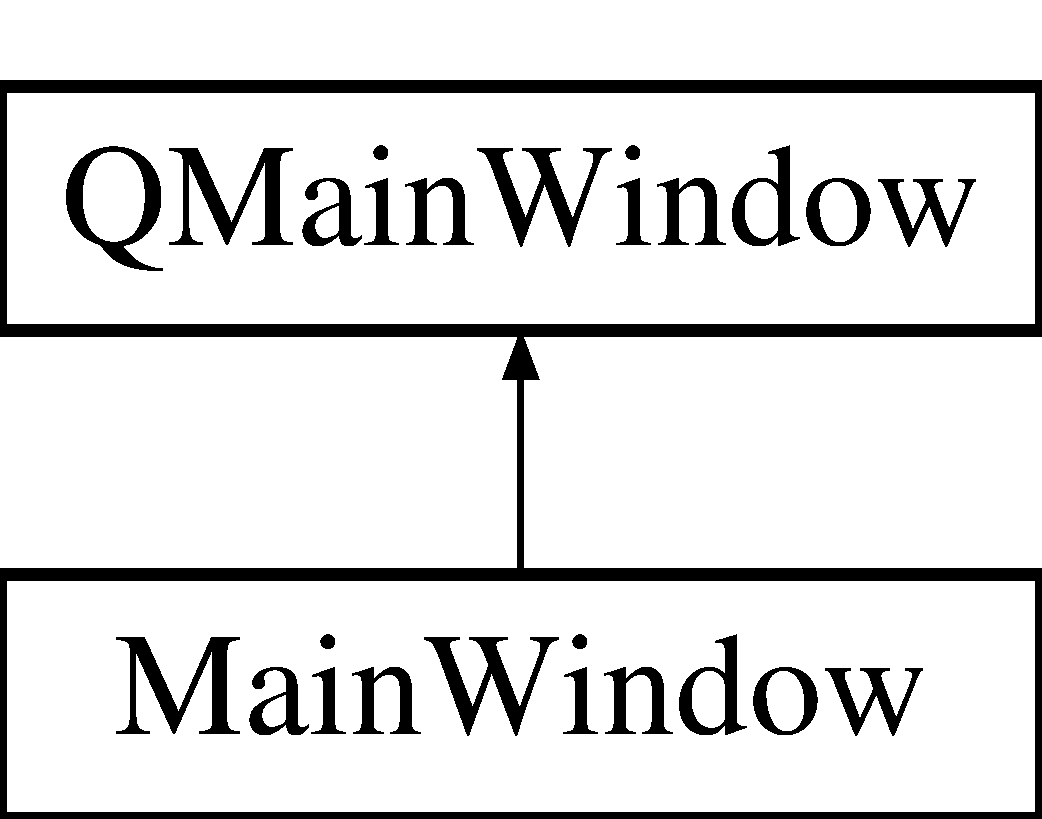
\includegraphics[height=2.000000cm]{class_main_window}
\end{center}
\end{figure}
\subsection*{Public Member Functions}
\begin{DoxyCompactItemize}
\item 
\mbox{\Hypertarget{class_main_window_a8b244be8b7b7db1b08de2a2acb9409db}\label{class_main_window_a8b244be8b7b7db1b08de2a2acb9409db}} 
{\bfseries Main\+Window} (Q\+Widget $\ast$parent=0)
\end{DoxyCompactItemize}


\subsection{Detailed Description}
The \hyperlink{class_main_window}{Main\+Window} class. 

The documentation for this class was generated from the following files\+:\begin{DoxyCompactItemize}
\item 
mainwindow.\+h\item 
mainwindow.\+cpp\end{DoxyCompactItemize}

\hypertarget{class_multi_editeur}{}\section{Multi\+Editeur Class Reference}
\label{class_multi_editeur}\index{Multi\+Editeur@{Multi\+Editeur}}


The \hyperlink{class_multi_editeur}{Multi\+Editeur} class permet afficher \hyperlink{class_multimedia}{Multimedia}, herite \hyperlink{class_note_editeur}{Note\+Editeur}.  




{\ttfamily \#include $<$noteediteur.\+h$>$}

Inheritance diagram for Multi\+Editeur\+:\begin{figure}[H]
\begin{center}
\leavevmode
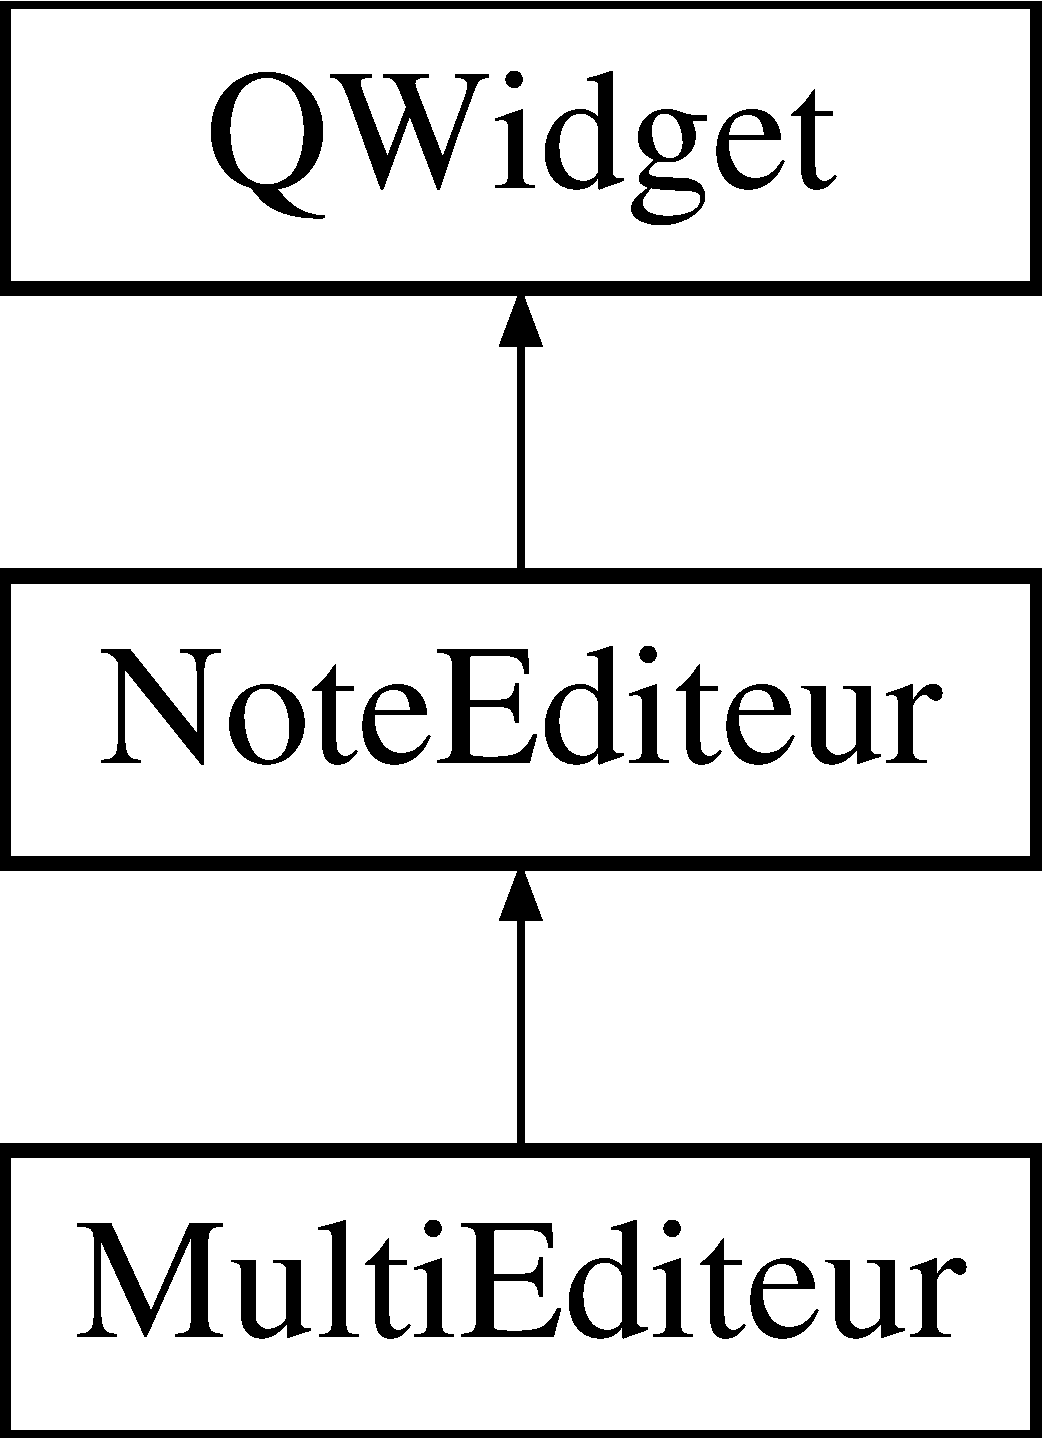
\includegraphics[height=3.000000cm]{class_multi_editeur}
\end{center}
\end{figure}
\subsection*{Public Slots}
\begin{DoxyCompactItemize}
\item 
\mbox{\Hypertarget{class_multi_editeur_a70904cb42da2463fdcd124fe42e47a68}\label{class_multi_editeur_a70904cb42da2463fdcd124fe42e47a68}} 
void \hyperlink{class_multi_editeur_a70904cb42da2463fdcd124fe42e47a68}{save\+Multi} ()
\begin{DoxyCompactList}\small\item\em save\+Multi enregistrer modif multimedia \end{DoxyCompactList}\item 
\mbox{\Hypertarget{class_multi_editeur_ade11724d5637738f716e913bfb707511}\label{class_multi_editeur_ade11724d5637738f716e913bfb707511}} 
void \hyperlink{class_multi_editeur_ade11724d5637738f716e913bfb707511}{archiver\+Multi} ()
\begin{DoxyCompactList}\small\item\em archiver\+Multi archiver un multimedia \end{DoxyCompactList}\item 
\mbox{\Hypertarget{class_multi_editeur_a201417424a9d8fac2828daa6b78388c3}\label{class_multi_editeur_a201417424a9d8fac2828daa6b78388c3}} 
void \hyperlink{class_multi_editeur_a201417424a9d8fac2828daa6b78388c3}{restaurer\+Multi} ()
\begin{DoxyCompactList}\small\item\em restaurer\+Multi restaurer un multimedia \end{DoxyCompactList}\end{DoxyCompactItemize}
\subsection*{Public Member Functions}
\begin{DoxyCompactItemize}
\item 
\hyperlink{class_multi_editeur_a7a3f689abaf2b3c5783c529128f67ad8}{Multi\+Editeur} (\hyperlink{class_multimedia}{Multimedia} \&multi, \hyperlink{class_fenetre_principale}{Fenetre\+Principale} $\ast$p)
\begin{DoxyCompactList}\small\item\em \hyperlink{class_multi_editeur}{Multi\+Editeur}. \end{DoxyCompactList}\item 
\hyperlink{class_multi_editeur_abc1f09828dc220dcf4cb45be5d94099d}{Multi\+Editeur} (\hyperlink{class_multimedia}{Multimedia} \&multi, \hyperlink{class_fenetre_principale}{Fenetre\+Principale} $\ast$p, int j)
\begin{DoxyCompactList}\small\item\em \hyperlink{class_multi_editeur}{Multi\+Editeur}. \end{DoxyCompactList}\end{DoxyCompactItemize}


\subsection{Detailed Description}
The \hyperlink{class_multi_editeur}{Multi\+Editeur} class permet afficher \hyperlink{class_multimedia}{Multimedia}, herite \hyperlink{class_note_editeur}{Note\+Editeur}. 

\subsection{Constructor \& Destructor Documentation}
\mbox{\Hypertarget{class_multi_editeur_a7a3f689abaf2b3c5783c529128f67ad8}\label{class_multi_editeur_a7a3f689abaf2b3c5783c529128f67ad8}} 
\index{Multi\+Editeur@{Multi\+Editeur}!Multi\+Editeur@{Multi\+Editeur}}
\index{Multi\+Editeur@{Multi\+Editeur}!Multi\+Editeur@{Multi\+Editeur}}
\subsubsection{\texorpdfstring{Multi\+Editeur()}{MultiEditeur()}\hspace{0.1cm}{\footnotesize\ttfamily [1/2]}}
{\footnotesize\ttfamily Multi\+Editeur\+::\+Multi\+Editeur (\begin{DoxyParamCaption}\item[{\hyperlink{class_multimedia}{Multimedia} \&}]{multi,  }\item[{\hyperlink{class_fenetre_principale}{Fenetre\+Principale} $\ast$}]{p }\end{DoxyParamCaption})}



\hyperlink{class_multi_editeur}{Multi\+Editeur}. 


\begin{DoxyParams}{Parameters}
{\em multi} & multimedia à afficher \\
\hline
{\em p} & \hyperlink{class_fenetre_principale}{Fenetre\+Principale} dans laquelle afficher \\
\hline
\end{DoxyParams}
\mbox{\Hypertarget{class_multi_editeur_abc1f09828dc220dcf4cb45be5d94099d}\label{class_multi_editeur_abc1f09828dc220dcf4cb45be5d94099d}} 
\index{Multi\+Editeur@{Multi\+Editeur}!Multi\+Editeur@{Multi\+Editeur}}
\index{Multi\+Editeur@{Multi\+Editeur}!Multi\+Editeur@{Multi\+Editeur}}
\subsubsection{\texorpdfstring{Multi\+Editeur()}{MultiEditeur()}\hspace{0.1cm}{\footnotesize\ttfamily [2/2]}}
{\footnotesize\ttfamily Multi\+Editeur\+::\+Multi\+Editeur (\begin{DoxyParamCaption}\item[{\hyperlink{class_multimedia}{Multimedia} \&}]{multi,  }\item[{\hyperlink{class_fenetre_principale}{Fenetre\+Principale} $\ast$}]{p,  }\item[{int}]{j }\end{DoxyParamCaption})}



\hyperlink{class_multi_editeur}{Multi\+Editeur}. 


\begin{DoxyParams}{Parameters}
{\em multi} & multimedia à afficher \\
\hline
{\em p} & \hyperlink{class_fenetre_principale}{Fenetre\+Principale} dans laquelle afficher \\
\hline
{\em j} & pour savoir si archive \\
\hline
\end{DoxyParams}


The documentation for this class was generated from the following files\+:\begin{DoxyCompactItemize}
\item 
noteediteur.\+h\item 
noteediteur.\+cpp\end{DoxyCompactItemize}

\hypertarget{class_multimedia}{}\section{Multimedia Class Reference}
\label{class_multimedia}\index{Multimedia@{Multimedia}}
Inheritance diagram for Multimedia\+:\begin{figure}[H]
\begin{center}
\leavevmode
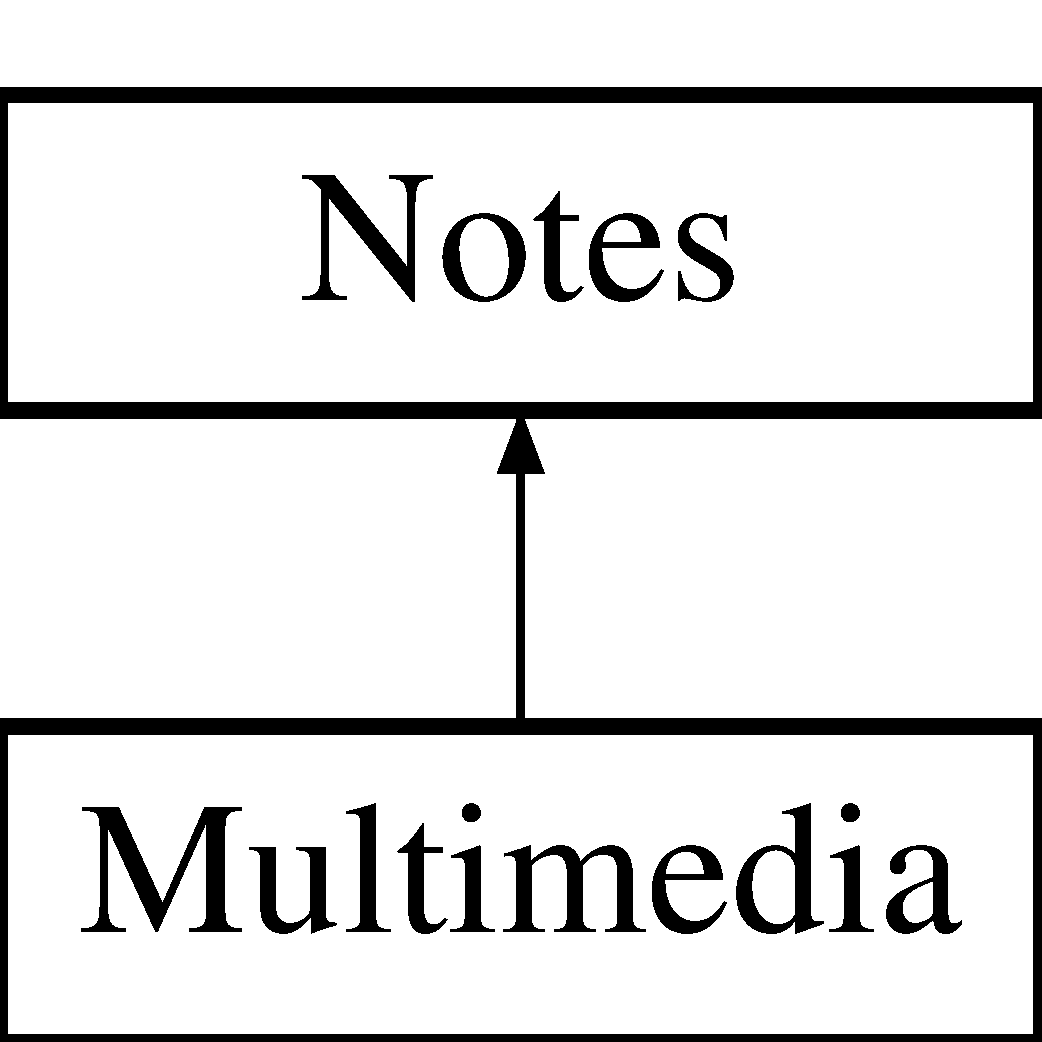
\includegraphics[height=2.000000cm]{class_multimedia}
\end{center}
\end{figure}
\subsection*{Public Member Functions}
\begin{DoxyCompactItemize}
\item 
const Q\+String \& \hyperlink{class_multimedia_a5036bb76fb0e9e0fc30fab727c2153bf}{get\+Desc} () const
\begin{DoxyCompactList}\small\item\em get\+Desc \end{DoxyCompactList}\item 
const Q\+String \& \hyperlink{class_multimedia_af104383032e12ecd6b4e44fefc6dd6b8}{get\+Fichier} () const
\begin{DoxyCompactList}\small\item\em get\+Fichier \end{DoxyCompactList}\item 
const Q\+String \& \hyperlink{class_multimedia_a2efca50fca32401a47da0438fc063cbf}{get\+Type} () const
\begin{DoxyCompactList}\small\item\em get\+Type \end{DoxyCompactList}\item 
void \hyperlink{class_multimedia_a69eeb6cd2fa096efd99193e2e2427765}{set\+Desc} (const Q\+String \&s)
\begin{DoxyCompactList}\small\item\em set\+Desc \end{DoxyCompactList}\item 
void \hyperlink{class_multimedia_a09e44004cbaa54f55b933cbdda12cb49}{set\+Fichier} (const Q\+String \&s)
\begin{DoxyCompactList}\small\item\em set\+Fichier \end{DoxyCompactList}\item 
void \hyperlink{class_multimedia_a1e0b015d47c6bbe7704f78d6b2470ecf}{set\+Type} (const Q\+String \&t)
\begin{DoxyCompactList}\small\item\em set\+Type \end{DoxyCompactList}\item 
\hyperlink{class_multimedia_ace2a9de6115c4d35f08468ed29af8a04}{Multimedia} (const Q\+String i, const Q\+String titr, const Q\+String desc, const Q\+String fich, const Q\+String typ)
\begin{DoxyCompactList}\small\item\em \hyperlink{class_multimedia}{Multimedia}. \end{DoxyCompactList}\item 
\hyperlink{class_multimedia_a891cf1d69986913d558a56029181c6f5}{Multimedia} (const Q\+String i, const Q\+String titr, const Q\+String desc, const Q\+String fich, const Q\+String typ, Q\+Date date\+Crea, Q\+Date date\+Modif)
\begin{DoxyCompactList}\small\item\em \hyperlink{class_multimedia}{Multimedia}. \end{DoxyCompactList}\item 
\mbox{\Hypertarget{class_multimedia_a61c05b6005500e320ffe313d9bb9374c}\label{class_multimedia_a61c05b6005500e320ffe313d9bb9374c}} 
void \hyperlink{class_multimedia_a61c05b6005500e320ffe313d9bb9374c}{afficher} ()
\begin{DoxyCompactList}\small\item\em afficher \end{DoxyCompactList}\end{DoxyCompactItemize}


\subsection{Constructor \& Destructor Documentation}
\mbox{\Hypertarget{class_multimedia_ace2a9de6115c4d35f08468ed29af8a04}\label{class_multimedia_ace2a9de6115c4d35f08468ed29af8a04}} 
\index{Multimedia@{Multimedia}!Multimedia@{Multimedia}}
\index{Multimedia@{Multimedia}!Multimedia@{Multimedia}}
\subsubsection{\texorpdfstring{Multimedia()}{Multimedia()}\hspace{0.1cm}{\footnotesize\ttfamily [1/2]}}
{\footnotesize\ttfamily Multimedia\+::\+Multimedia (\begin{DoxyParamCaption}\item[{const Q\+String}]{i,  }\item[{const Q\+String}]{titr,  }\item[{const Q\+String}]{desc,  }\item[{const Q\+String}]{fich,  }\item[{const Q\+String}]{typ }\end{DoxyParamCaption})\hspace{0.3cm}{\ttfamily [inline]}}



\hyperlink{class_multimedia}{Multimedia}. 


\begin{DoxyParams}{Parameters}
{\em i} & \\
\hline
{\em titr} & \\
\hline
{\em desc} & \\
\hline
{\em fich} & \\
\hline
{\em typ} & constructeur \\
\hline
\end{DoxyParams}
\mbox{\Hypertarget{class_multimedia_a891cf1d69986913d558a56029181c6f5}\label{class_multimedia_a891cf1d69986913d558a56029181c6f5}} 
\index{Multimedia@{Multimedia}!Multimedia@{Multimedia}}
\index{Multimedia@{Multimedia}!Multimedia@{Multimedia}}
\subsubsection{\texorpdfstring{Multimedia()}{Multimedia()}\hspace{0.1cm}{\footnotesize\ttfamily [2/2]}}
{\footnotesize\ttfamily Multimedia\+::\+Multimedia (\begin{DoxyParamCaption}\item[{const Q\+String}]{i,  }\item[{const Q\+String}]{titr,  }\item[{const Q\+String}]{desc,  }\item[{const Q\+String}]{fich,  }\item[{const Q\+String}]{typ,  }\item[{Q\+Date}]{date\+Crea,  }\item[{Q\+Date}]{date\+Modif }\end{DoxyParamCaption})\hspace{0.3cm}{\ttfamily [inline]}}



\hyperlink{class_multimedia}{Multimedia}. 


\begin{DoxyParams}{Parameters}
{\em i} & \\
\hline
{\em titr} & \\
\hline
{\em desc} & \\
\hline
{\em fich} & \\
\hline
{\em typ} & \\
\hline
{\em date\+Crea} & \\
\hline
{\em date\+Modif} & surcharge du constructeur \\
\hline
\end{DoxyParams}


\subsection{Member Function Documentation}
\mbox{\Hypertarget{class_multimedia_a5036bb76fb0e9e0fc30fab727c2153bf}\label{class_multimedia_a5036bb76fb0e9e0fc30fab727c2153bf}} 
\index{Multimedia@{Multimedia}!get\+Desc@{get\+Desc}}
\index{get\+Desc@{get\+Desc}!Multimedia@{Multimedia}}
\subsubsection{\texorpdfstring{get\+Desc()}{getDesc()}}
{\footnotesize\ttfamily const Q\+String\& Multimedia\+::get\+Desc (\begin{DoxyParamCaption}{ }\end{DoxyParamCaption}) const\hspace{0.3cm}{\ttfamily [inline]}}



get\+Desc 

\begin{DoxyReturn}{Returns}

\end{DoxyReturn}
\mbox{\Hypertarget{class_multimedia_af104383032e12ecd6b4e44fefc6dd6b8}\label{class_multimedia_af104383032e12ecd6b4e44fefc6dd6b8}} 
\index{Multimedia@{Multimedia}!get\+Fichier@{get\+Fichier}}
\index{get\+Fichier@{get\+Fichier}!Multimedia@{Multimedia}}
\subsubsection{\texorpdfstring{get\+Fichier()}{getFichier()}}
{\footnotesize\ttfamily const Q\+String\& Multimedia\+::get\+Fichier (\begin{DoxyParamCaption}{ }\end{DoxyParamCaption}) const\hspace{0.3cm}{\ttfamily [inline]}}



get\+Fichier 

\begin{DoxyReturn}{Returns}

\end{DoxyReturn}
\mbox{\Hypertarget{class_multimedia_a2efca50fca32401a47da0438fc063cbf}\label{class_multimedia_a2efca50fca32401a47da0438fc063cbf}} 
\index{Multimedia@{Multimedia}!get\+Type@{get\+Type}}
\index{get\+Type@{get\+Type}!Multimedia@{Multimedia}}
\subsubsection{\texorpdfstring{get\+Type()}{getType()}}
{\footnotesize\ttfamily const Q\+String\& Multimedia\+::get\+Type (\begin{DoxyParamCaption}{ }\end{DoxyParamCaption}) const\hspace{0.3cm}{\ttfamily [inline]}}



get\+Type 

\begin{DoxyReturn}{Returns}

\end{DoxyReturn}
\mbox{\Hypertarget{class_multimedia_a69eeb6cd2fa096efd99193e2e2427765}\label{class_multimedia_a69eeb6cd2fa096efd99193e2e2427765}} 
\index{Multimedia@{Multimedia}!set\+Desc@{set\+Desc}}
\index{set\+Desc@{set\+Desc}!Multimedia@{Multimedia}}
\subsubsection{\texorpdfstring{set\+Desc()}{setDesc()}}
{\footnotesize\ttfamily void Multimedia\+::set\+Desc (\begin{DoxyParamCaption}\item[{const Q\+String \&}]{s }\end{DoxyParamCaption})\hspace{0.3cm}{\ttfamily [inline]}}



set\+Desc 


\begin{DoxyParams}{Parameters}
{\em s} & \\
\hline
\end{DoxyParams}
\mbox{\Hypertarget{class_multimedia_a09e44004cbaa54f55b933cbdda12cb49}\label{class_multimedia_a09e44004cbaa54f55b933cbdda12cb49}} 
\index{Multimedia@{Multimedia}!set\+Fichier@{set\+Fichier}}
\index{set\+Fichier@{set\+Fichier}!Multimedia@{Multimedia}}
\subsubsection{\texorpdfstring{set\+Fichier()}{setFichier()}}
{\footnotesize\ttfamily void Multimedia\+::set\+Fichier (\begin{DoxyParamCaption}\item[{const Q\+String \&}]{s }\end{DoxyParamCaption})\hspace{0.3cm}{\ttfamily [inline]}}



set\+Fichier 


\begin{DoxyParams}{Parameters}
{\em s} & \\
\hline
\end{DoxyParams}
\mbox{\Hypertarget{class_multimedia_a1e0b015d47c6bbe7704f78d6b2470ecf}\label{class_multimedia_a1e0b015d47c6bbe7704f78d6b2470ecf}} 
\index{Multimedia@{Multimedia}!set\+Type@{set\+Type}}
\index{set\+Type@{set\+Type}!Multimedia@{Multimedia}}
\subsubsection{\texorpdfstring{set\+Type()}{setType()}}
{\footnotesize\ttfamily void Multimedia\+::set\+Type (\begin{DoxyParamCaption}\item[{const Q\+String \&}]{t }\end{DoxyParamCaption})\hspace{0.3cm}{\ttfamily [inline]}}



set\+Type 


\begin{DoxyParams}{Parameters}
{\em t} & \\
\hline
\end{DoxyParams}


The documentation for this class was generated from the following files\+:\begin{DoxyCompactItemize}
\item 
notes.\+h\item 
notes.\+cpp\end{DoxyCompactItemize}

\hypertarget{class_note_editeur}{}\section{Note\+Editeur Class Reference}
\label{class_note_editeur}\index{Note\+Editeur@{Note\+Editeur}}


The \hyperlink{class_note_editeur}{Note\+Editeur} class permet afficher partie note d\textquotesingle{}un article, tache ou multi.  




{\ttfamily \#include $<$noteediteur.\+h$>$}

Inheritance diagram for Note\+Editeur\+:\begin{figure}[H]
\begin{center}
\leavevmode
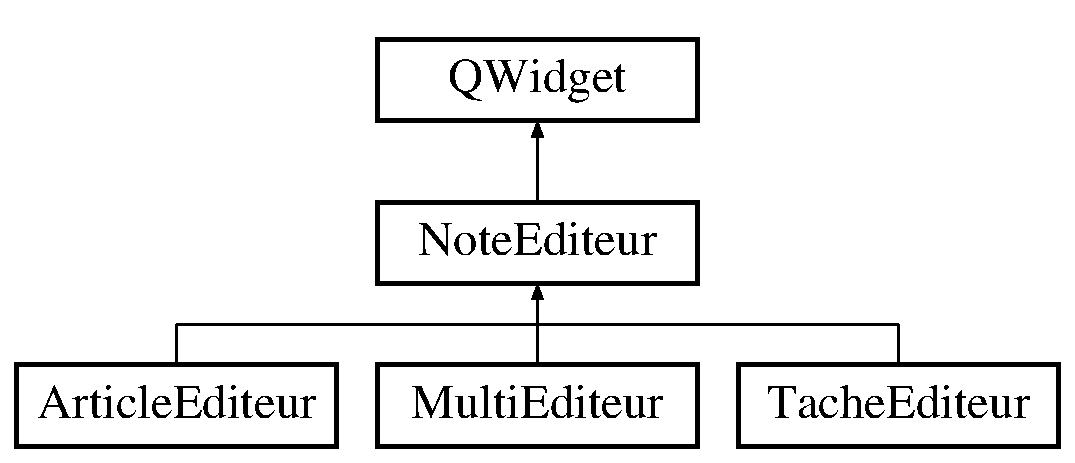
\includegraphics[height=3.000000cm]{class_note_editeur}
\end{center}
\end{figure}
\subsection*{Public Member Functions}
\begin{DoxyCompactItemize}
\item 
\hyperlink{class_note_editeur_a5488a0e9553714cf8232f9ca56305e23}{Note\+Editeur} (\hyperlink{class_notes}{Notes} \&n, \hyperlink{class_fenetre_principale}{Fenetre\+Principale} $\ast$p)
\begin{DoxyCompactList}\small\item\em \hyperlink{class_note_editeur}{Note\+Editeur}. \end{DoxyCompactList}\item 
\mbox{\Hypertarget{class_note_editeur_ae4689219a596cc159e22d524fea6c995}\label{class_note_editeur_ae4689219a596cc159e22d524fea6c995}} 
{\bfseries Note\+Editeur} (\hyperlink{class_fenetre_principale}{Fenetre\+Principale} $\ast$p)
\item 
\mbox{\Hypertarget{class_note_editeur_a438c4a989e222d3fcbd04fd960e24776}\label{class_note_editeur_a438c4a989e222d3fcbd04fd960e24776}} 
Q\+V\+Box\+Layout $\ast$ {\bfseries get\+Couche} ()
\item 
\mbox{\Hypertarget{class_note_editeur_a5b1566a2019f8717a4648e61997ad058}\label{class_note_editeur_a5b1566a2019f8717a4648e61997ad058}} 
Q\+String {\bfseries get\+Titre} ()
\item 
\mbox{\Hypertarget{class_note_editeur_aab9454ecfabe432c22e54d531b716b0c}\label{class_note_editeur_aab9454ecfabe432c22e54d531b716b0c}} 
Q\+Line\+Edit $\ast$ {\bfseries Titre} ()
\item 
\mbox{\Hypertarget{class_note_editeur_a0d713ee7aae120ceac4388ac6de269f8}\label{class_note_editeur_a0d713ee7aae120ceac4388ac6de269f8}} 
\hyperlink{class_fenetre_principale}{Fenetre\+Principale} $\ast$ {\bfseries get\+Pere} ()
\end{DoxyCompactItemize}


\subsection{Detailed Description}
The \hyperlink{class_note_editeur}{Note\+Editeur} class permet afficher partie note d\textquotesingle{}un article, tache ou multi. 

\subsection{Constructor \& Destructor Documentation}
\mbox{\Hypertarget{class_note_editeur_a5488a0e9553714cf8232f9ca56305e23}\label{class_note_editeur_a5488a0e9553714cf8232f9ca56305e23}} 
\index{Note\+Editeur@{Note\+Editeur}!Note\+Editeur@{Note\+Editeur}}
\index{Note\+Editeur@{Note\+Editeur}!Note\+Editeur@{Note\+Editeur}}
\subsubsection{\texorpdfstring{Note\+Editeur()}{NoteEditeur()}}
{\footnotesize\ttfamily Note\+Editeur\+::\+Note\+Editeur (\begin{DoxyParamCaption}\item[{\hyperlink{class_notes}{Notes} \&}]{n,  }\item[{\hyperlink{class_fenetre_principale}{Fenetre\+Principale} $\ast$}]{p }\end{DoxyParamCaption})}



\hyperlink{class_note_editeur}{Note\+Editeur}. 


\begin{DoxyParams}{Parameters}
{\em n} & note a afficher \\
\hline
{\em p} & \hyperlink{class_fenetre_principale}{Fenetre\+Principale} dans laquelle afficher \\
\hline
\end{DoxyParams}


The documentation for this class was generated from the following files\+:\begin{DoxyCompactItemize}
\item 
noteediteur.\+h\item 
noteediteur.\+cpp\end{DoxyCompactItemize}

\hypertarget{class_notes}{}\section{Notes Class Reference}
\label{class_notes}\index{Notes@{Notes}}


The \hyperlink{class_notes}{Notes} class Classe abstraite.  




{\ttfamily \#include $<$notes.\+h$>$}

Inheritance diagram for Notes\+:\begin{figure}[H]
\begin{center}
\leavevmode
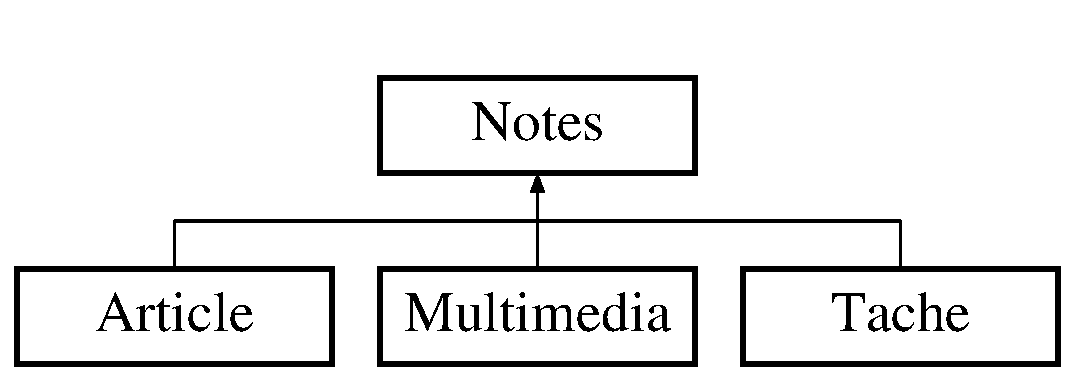
\includegraphics[height=2.000000cm]{class_notes}
\end{center}
\end{figure}
\subsection*{Public Member Functions}
\begin{DoxyCompactItemize}
\item 
\hyperlink{class_notes_aff3e54629e3e1005aafc512f87c8aa8f}{Notes} (const Q\+String i, const Q\+String t)
\begin{DoxyCompactList}\small\item\em \hyperlink{class_notes}{Notes}. \end{DoxyCompactList}\item 
\hyperlink{class_notes_ab19ca69e24270ac6fd5b92c304a1bf1b}{Notes} (const Q\+String i, const Q\+String t, const Q\+Date date\+Modif, const Q\+Date date\+Crea)
\begin{DoxyCompactList}\small\item\em \hyperlink{class_notes}{Notes}. \end{DoxyCompactList}\item 
\mbox{\Hypertarget{class_notes_ac5829fca5044dea12bb3290fd1c6d86d}\label{class_notes_ac5829fca5044dea12bb3290fd1c6d86d}} 
virtual void \hyperlink{class_notes_ac5829fca5044dea12bb3290fd1c6d86d}{afficher} ()=0
\begin{DoxyCompactList}\small\item\em afficher methode virtuelle pure (on a oublié de s\textquotesingle{}en servir dans les classes filles) \end{DoxyCompactList}\item 
const Q\+String \& \hyperlink{class_notes_a034e1fb763f1535b245fed61f2c07eaa}{get\+Id} () const
\begin{DoxyCompactList}\small\item\em get\+Id \end{DoxyCompactList}\item 
const Q\+String \& \hyperlink{class_notes_ad62548dca78862addfbe7c8a0b797c82}{get\+Titre} () const
\begin{DoxyCompactList}\small\item\em get\+Titre \end{DoxyCompactList}\item 
const Q\+Date \& \hyperlink{class_notes_ae375538696f0a9c0cbe446900d3eaf6e}{get\+Modif} () const
\begin{DoxyCompactList}\small\item\em get\+Modif \end{DoxyCompactList}\item 
const Q\+Date \& \hyperlink{class_notes_a0e396bd4a81ceaa93e7f7d829a3047e2}{get\+Crea} () const
\begin{DoxyCompactList}\small\item\em get\+Crea \end{DoxyCompactList}\item 
void \hyperlink{class_notes_a31e62febfc96b4b1a4ed33647c193f93}{set\+Titre} (const Q\+String \&s)
\begin{DoxyCompactList}\small\item\em set\+Titre \end{DoxyCompactList}\item 
void \hyperlink{class_notes_a903b6acb849c7aa9ba25161106f31299}{set\+Modif} (const Q\+Date \&d)
\begin{DoxyCompactList}\small\item\em set\+Modif \end{DoxyCompactList}\item 
void \hyperlink{class_notes_aade3f1a559f3df47181b746a47e93a72}{set\+Crea} (const Q\+Date \&d)
\begin{DoxyCompactList}\small\item\em set\+Crea \end{DoxyCompactList}\item 
bool \hyperlink{class_notes_abf74367554c664c909f14f752a544384}{operator==} (const \hyperlink{class_notes}{Notes} \&n)
\begin{DoxyCompactList}\small\item\em operator == \end{DoxyCompactList}\end{DoxyCompactItemize}


\subsection{Detailed Description}
The \hyperlink{class_notes}{Notes} class Classe abstraite. 

\subsection{Constructor \& Destructor Documentation}
\mbox{\Hypertarget{class_notes_aff3e54629e3e1005aafc512f87c8aa8f}\label{class_notes_aff3e54629e3e1005aafc512f87c8aa8f}} 
\index{Notes@{Notes}!Notes@{Notes}}
\index{Notes@{Notes}!Notes@{Notes}}
\subsubsection{\texorpdfstring{Notes()}{Notes()}\hspace{0.1cm}{\footnotesize\ttfamily [1/2]}}
{\footnotesize\ttfamily Notes\+::\+Notes (\begin{DoxyParamCaption}\item[{const Q\+String}]{i,  }\item[{const Q\+String}]{t }\end{DoxyParamCaption})\hspace{0.3cm}{\ttfamily [inline]}}



\hyperlink{class_notes}{Notes}. 


\begin{DoxyParams}{Parameters}
{\em i} & id \\
\hline
{\em t} & titre et initialise date de creation et date de dernière modification avec la date actuelle \\
\hline
\end{DoxyParams}
\mbox{\Hypertarget{class_notes_ab19ca69e24270ac6fd5b92c304a1bf1b}\label{class_notes_ab19ca69e24270ac6fd5b92c304a1bf1b}} 
\index{Notes@{Notes}!Notes@{Notes}}
\index{Notes@{Notes}!Notes@{Notes}}
\subsubsection{\texorpdfstring{Notes()}{Notes()}\hspace{0.1cm}{\footnotesize\ttfamily [2/2]}}
{\footnotesize\ttfamily Notes\+::\+Notes (\begin{DoxyParamCaption}\item[{const Q\+String}]{i,  }\item[{const Q\+String}]{t,  }\item[{const Q\+Date}]{date\+Modif,  }\item[{const Q\+Date}]{date\+Crea }\end{DoxyParamCaption})\hspace{0.3cm}{\ttfamily [inline]}}



\hyperlink{class_notes}{Notes}. 


\begin{DoxyParams}{Parameters}
{\em i} & \\
\hline
{\em t} & \\
\hline
{\em date\+Modif} & \\
\hline
{\em date\+Crea} & surcharge constructeur pour methode load() \\
\hline
\end{DoxyParams}


\subsection{Member Function Documentation}
\mbox{\Hypertarget{class_notes_a0e396bd4a81ceaa93e7f7d829a3047e2}\label{class_notes_a0e396bd4a81ceaa93e7f7d829a3047e2}} 
\index{Notes@{Notes}!get\+Crea@{get\+Crea}}
\index{get\+Crea@{get\+Crea}!Notes@{Notes}}
\subsubsection{\texorpdfstring{get\+Crea()}{getCrea()}}
{\footnotesize\ttfamily const Q\+Date\& Notes\+::get\+Crea (\begin{DoxyParamCaption}{ }\end{DoxyParamCaption}) const\hspace{0.3cm}{\ttfamily [inline]}}



get\+Crea 

\begin{DoxyReturn}{Returns}
la date de creation accesseur en lecture 
\end{DoxyReturn}
\mbox{\Hypertarget{class_notes_a034e1fb763f1535b245fed61f2c07eaa}\label{class_notes_a034e1fb763f1535b245fed61f2c07eaa}} 
\index{Notes@{Notes}!get\+Id@{get\+Id}}
\index{get\+Id@{get\+Id}!Notes@{Notes}}
\subsubsection{\texorpdfstring{get\+Id()}{getId()}}
{\footnotesize\ttfamily const Q\+String\& Notes\+::get\+Id (\begin{DoxyParamCaption}{ }\end{DoxyParamCaption}) const\hspace{0.3cm}{\ttfamily [inline]}}



get\+Id 

\begin{DoxyReturn}{Returns}
identifiant de la note accesseur en lecture 
\end{DoxyReturn}
\mbox{\Hypertarget{class_notes_ae375538696f0a9c0cbe446900d3eaf6e}\label{class_notes_ae375538696f0a9c0cbe446900d3eaf6e}} 
\index{Notes@{Notes}!get\+Modif@{get\+Modif}}
\index{get\+Modif@{get\+Modif}!Notes@{Notes}}
\subsubsection{\texorpdfstring{get\+Modif()}{getModif()}}
{\footnotesize\ttfamily const Q\+Date\& Notes\+::get\+Modif (\begin{DoxyParamCaption}{ }\end{DoxyParamCaption}) const\hspace{0.3cm}{\ttfamily [inline]}}



get\+Modif 

\begin{DoxyReturn}{Returns}
la date de dernière modif accesseur en lecture 
\end{DoxyReturn}
\mbox{\Hypertarget{class_notes_ad62548dca78862addfbe7c8a0b797c82}\label{class_notes_ad62548dca78862addfbe7c8a0b797c82}} 
\index{Notes@{Notes}!get\+Titre@{get\+Titre}}
\index{get\+Titre@{get\+Titre}!Notes@{Notes}}
\subsubsection{\texorpdfstring{get\+Titre()}{getTitre()}}
{\footnotesize\ttfamily const Q\+String\& Notes\+::get\+Titre (\begin{DoxyParamCaption}{ }\end{DoxyParamCaption}) const\hspace{0.3cm}{\ttfamily [inline]}}



get\+Titre 

\begin{DoxyReturn}{Returns}
titre de la note accesseur en lecture 
\end{DoxyReturn}
\mbox{\Hypertarget{class_notes_abf74367554c664c909f14f752a544384}\label{class_notes_abf74367554c664c909f14f752a544384}} 
\index{Notes@{Notes}!operator==@{operator==}}
\index{operator==@{operator==}!Notes@{Notes}}
\subsubsection{\texorpdfstring{operator==()}{operator==()}}
{\footnotesize\ttfamily bool Notes\+::operator== (\begin{DoxyParamCaption}\item[{const \hyperlink{class_notes}{Notes} \&}]{n }\end{DoxyParamCaption})}



operator == 


\begin{DoxyParams}{Parameters}
{\em n} & \\
\hline
\end{DoxyParams}
\begin{DoxyReturn}{Returns}
bool surcharge operator== 
\end{DoxyReturn}
\mbox{\Hypertarget{class_notes_aade3f1a559f3df47181b746a47e93a72}\label{class_notes_aade3f1a559f3df47181b746a47e93a72}} 
\index{Notes@{Notes}!set\+Crea@{set\+Crea}}
\index{set\+Crea@{set\+Crea}!Notes@{Notes}}
\subsubsection{\texorpdfstring{set\+Crea()}{setCrea()}}
{\footnotesize\ttfamily void Notes\+::set\+Crea (\begin{DoxyParamCaption}\item[{const Q\+Date \&}]{d }\end{DoxyParamCaption})\hspace{0.3cm}{\ttfamily [inline]}}



set\+Crea 


\begin{DoxyParams}{Parameters}
{\em d} & accesseur en ecriture pour date crea \\
\hline
\end{DoxyParams}
\mbox{\Hypertarget{class_notes_a903b6acb849c7aa9ba25161106f31299}\label{class_notes_a903b6acb849c7aa9ba25161106f31299}} 
\index{Notes@{Notes}!set\+Modif@{set\+Modif}}
\index{set\+Modif@{set\+Modif}!Notes@{Notes}}
\subsubsection{\texorpdfstring{set\+Modif()}{setModif()}}
{\footnotesize\ttfamily void Notes\+::set\+Modif (\begin{DoxyParamCaption}\item[{const Q\+Date \&}]{d }\end{DoxyParamCaption})\hspace{0.3cm}{\ttfamily [inline]}}



set\+Modif 


\begin{DoxyParams}{Parameters}
{\em d} & accesseur en ecriture pour date modif \\
\hline
\end{DoxyParams}
\mbox{\Hypertarget{class_notes_a31e62febfc96b4b1a4ed33647c193f93}\label{class_notes_a31e62febfc96b4b1a4ed33647c193f93}} 
\index{Notes@{Notes}!set\+Titre@{set\+Titre}}
\index{set\+Titre@{set\+Titre}!Notes@{Notes}}
\subsubsection{\texorpdfstring{set\+Titre()}{setTitre()}}
{\footnotesize\ttfamily void Notes\+::set\+Titre (\begin{DoxyParamCaption}\item[{const Q\+String \&}]{s }\end{DoxyParamCaption})\hspace{0.3cm}{\ttfamily [inline]}}



set\+Titre 


\begin{DoxyParams}{Parameters}
{\em s} & accesseur en ecriture \\
\hline
\end{DoxyParams}


The documentation for this class was generated from the following files\+:\begin{DoxyCompactItemize}
\item 
notes.\+h\item 
notes.\+cpp\end{DoxyCompactItemize}

\hypertarget{class_relation}{}\section{Relation Class Reference}
\label{class_relation}\index{Relation@{Relation}}


The \hyperlink{class_relation}{Relation} class Classe abstraite.  




{\ttfamily \#include $<$relation.\+h$>$}

Inheritance diagram for Relation\+:\begin{figure}[H]
\begin{center}
\leavevmode
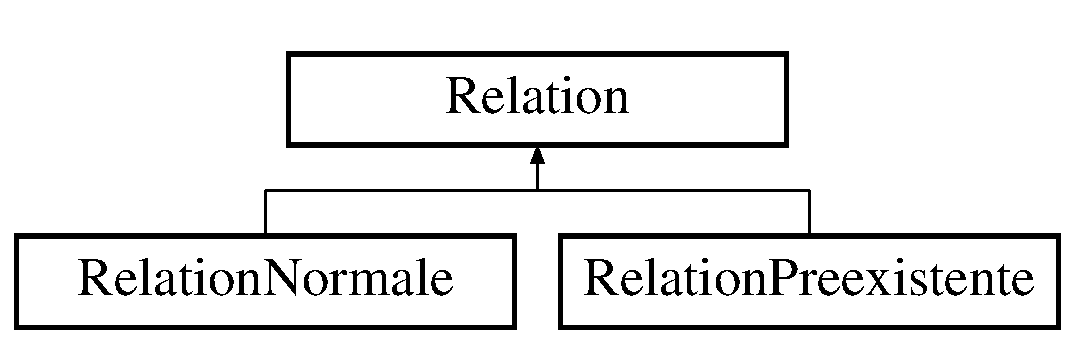
\includegraphics[height=2.000000cm]{class_relation}
\end{center}
\end{figure}
\subsection*{Classes}
\begin{DoxyCompactItemize}
\item 
class \hyperlink{class_relation_1_1iterator}{iterator}
\begin{DoxyCompactList}\small\item\em The iterator class pour parcourir les couples d\textquotesingle{}une relation. \end{DoxyCompactList}\end{DoxyCompactItemize}
\subsection*{Public Member Functions}
\begin{DoxyCompactItemize}
\item 
\hyperlink{class_relation_afded55b4b4ae7b23a86f280ad8b49369}{Relation} (const Q\+String \&id, const Q\+String \&titr, const Q\+String \&desc, bool orie=true)
\begin{DoxyCompactList}\small\item\em \hyperlink{class_relation}{Relation}. \end{DoxyCompactList}\item 
void \hyperlink{class_relation_a24e1e3542e1d5b133cd0850e939928b6}{add\+Couple} (\hyperlink{class_couple}{Couple} $\ast$new\+Couple)
\begin{DoxyCompactList}\small\item\em add\+Couple \end{DoxyCompactList}\item 
void \hyperlink{class_relation_a6d7a04daa6d55ff4e4fc3f8de2c168c5}{add\+Couple} (\hyperlink{class_notes}{Notes} \&n1, \hyperlink{class_notes}{Notes} \&n2, Q\+String l=\char`\"{}\char`\"{})
\begin{DoxyCompactList}\small\item\em add\+Couple \end{DoxyCompactList}\item 
const Q\+String \& \hyperlink{class_relation_a928c6b7afd86cbba6c7510e7495aa943}{get\+Id} () const
\begin{DoxyCompactList}\small\item\em get\+Id \end{DoxyCompactList}\item 
const Q\+String \& \hyperlink{class_relation_a411be3a1dfc417342db768555a2afe41}{get\+Titre} () const
\begin{DoxyCompactList}\small\item\em get\+Titre \end{DoxyCompactList}\item 
const Q\+String \& \hyperlink{class_relation_a078c6c43b163152aa40a9ac535175b9e}{get\+Description} () const
\begin{DoxyCompactList}\small\item\em get\+Description \end{DoxyCompactList}\item 
bool \hyperlink{class_relation_a77b7d698e607457ef5b14ded5d0e6f7f}{get\+Orientation} () const
\begin{DoxyCompactList}\small\item\em get\+Orientation \end{DoxyCompactList}\item 
virtual void \hyperlink{class_relation_a1c08a802796f5fccaa5732ec1a96e542}{set\+Titre} (const Q\+String \&new\+Titre)=0
\begin{DoxyCompactList}\small\item\em set\+Titre \end{DoxyCompactList}\item 
virtual void \hyperlink{class_relation_a8f698cc45c38a849c4bcd8336fa5e2b3}{set\+Description} (const Q\+String \&new\+Description)=0
\begin{DoxyCompactList}\small\item\em set\+Description \end{DoxyCompactList}\item 
virtual void \hyperlink{class_relation_a708a16e5b0dd280e64832ca1d042cd96}{set\+Orientation} (bool bool\+Val)=0
\begin{DoxyCompactList}\small\item\em set\+Orientation \end{DoxyCompactList}\item 
\mbox{\Hypertarget{class_relation_aac587ec926df3043c3eedcb5123be50b}\label{class_relation_aac587ec926df3043c3eedcb5123be50b}} 
virtual \hyperlink{class_relation_aac587ec926df3043c3eedcb5123be50b}{$\sim$\+Relation} ()
\begin{DoxyCompactList}\small\item\em $\sim$\+Relation gère la destruction des couples qui compose la relation \end{DoxyCompactList}\item 
\hyperlink{class_relation_1_1iterator}{iterator} \hyperlink{class_relation_a59d7e086b7a83b3aa7ca7a4a6adf8240}{begin\+\_\+relationr} ()
\begin{DoxyCompactList}\small\item\em begin\+\_\+relationr \end{DoxyCompactList}\item 
\hyperlink{class_relation_1_1iterator}{iterator} \hyperlink{class_relation_a2dca1dae07627e8e470d01fa95a7fb12}{end\+\_\+relation} ()
\begin{DoxyCompactList}\small\item\em end\+\_\+relation \end{DoxyCompactList}\end{DoxyCompactItemize}
\subsection*{Protected Attributes}
\begin{DoxyCompactItemize}
\item 
\mbox{\Hypertarget{class_relation_a8ebffdbe30936c6b9ca55781347b54d5}\label{class_relation_a8ebffdbe30936c6b9ca55781347b54d5}} 
Q\+String {\bfseries id}
\item 
\mbox{\Hypertarget{class_relation_a346e9b10df6757dee8dc13cb2f876357}\label{class_relation_a346e9b10df6757dee8dc13cb2f876357}} 
Q\+String {\bfseries titre}
\item 
\mbox{\Hypertarget{class_relation_a1140829291bd04a86d0b840524692703}\label{class_relation_a1140829291bd04a86d0b840524692703}} 
Q\+String {\bfseries description}
\item 
\mbox{\Hypertarget{class_relation_ae95d700e20c27e4123fdae4ef06923e0}\label{class_relation_ae95d700e20c27e4123fdae4ef06923e0}} 
bool {\bfseries orientation}
\end{DoxyCompactItemize}


\subsection{Detailed Description}
The \hyperlink{class_relation}{Relation} class Classe abstraite. 

\subsection{Constructor \& Destructor Documentation}
\mbox{\Hypertarget{class_relation_afded55b4b4ae7b23a86f280ad8b49369}\label{class_relation_afded55b4b4ae7b23a86f280ad8b49369}} 
\index{Relation@{Relation}!Relation@{Relation}}
\index{Relation@{Relation}!Relation@{Relation}}
\subsubsection{\texorpdfstring{Relation()}{Relation()}}
{\footnotesize\ttfamily Relation\+::\+Relation (\begin{DoxyParamCaption}\item[{const Q\+String \&}]{id,  }\item[{const Q\+String \&}]{titr,  }\item[{const Q\+String \&}]{desc,  }\item[{bool}]{orie = {\ttfamily true} }\end{DoxyParamCaption})\hspace{0.3cm}{\ttfamily [inline]}}



\hyperlink{class_relation}{Relation}. 


\begin{DoxyParams}{Parameters}
{\em id} & \\
\hline
{\em titr} & \\
\hline
{\em desc} & \\
\hline
{\em orie} & constructeur \\
\hline
\end{DoxyParams}


\subsection{Member Function Documentation}
\mbox{\Hypertarget{class_relation_a24e1e3542e1d5b133cd0850e939928b6}\label{class_relation_a24e1e3542e1d5b133cd0850e939928b6}} 
\index{Relation@{Relation}!add\+Couple@{add\+Couple}}
\index{add\+Couple@{add\+Couple}!Relation@{Relation}}
\subsubsection{\texorpdfstring{add\+Couple()}{addCouple()}\hspace{0.1cm}{\footnotesize\ttfamily [1/2]}}
{\footnotesize\ttfamily void Relation\+::add\+Couple (\begin{DoxyParamCaption}\item[{\hyperlink{class_couple}{Couple} $\ast$}]{new\+Couple }\end{DoxyParamCaption})}



add\+Couple 


\begin{DoxyParams}{Parameters}
{\em new\+Couple} & ajoute un couple au tableau couples \\
\hline
\end{DoxyParams}
\mbox{\Hypertarget{class_relation_a6d7a04daa6d55ff4e4fc3f8de2c168c5}\label{class_relation_a6d7a04daa6d55ff4e4fc3f8de2c168c5}} 
\index{Relation@{Relation}!add\+Couple@{add\+Couple}}
\index{add\+Couple@{add\+Couple}!Relation@{Relation}}
\subsubsection{\texorpdfstring{add\+Couple()}{addCouple()}\hspace{0.1cm}{\footnotesize\ttfamily [2/2]}}
{\footnotesize\ttfamily void Relation\+::add\+Couple (\begin{DoxyParamCaption}\item[{\hyperlink{class_notes}{Notes} \&}]{n1,  }\item[{\hyperlink{class_notes}{Notes} \&}]{n2,  }\item[{Q\+String}]{l = {\ttfamily \char`\"{}\char`\"{}} }\end{DoxyParamCaption})}



add\+Couple 


\begin{DoxyParams}{Parameters}
{\em n1} & \\
\hline
{\em n2} & \\
\hline
{\em l} & crée à partir de 2 notes et ajoute le couple au tableau couples \\
\hline
\end{DoxyParams}
\mbox{\Hypertarget{class_relation_a59d7e086b7a83b3aa7ca7a4a6adf8240}\label{class_relation_a59d7e086b7a83b3aa7ca7a4a6adf8240}} 
\index{Relation@{Relation}!begin\+\_\+relationr@{begin\+\_\+relationr}}
\index{begin\+\_\+relationr@{begin\+\_\+relationr}!Relation@{Relation}}
\subsubsection{\texorpdfstring{begin\+\_\+relationr()}{begin\_relationr()}}
{\footnotesize\ttfamily \hyperlink{class_relation_1_1iterator}{iterator} Relation\+::begin\+\_\+relationr (\begin{DoxyParamCaption}{ }\end{DoxyParamCaption})\hspace{0.3cm}{\ttfamily [inline]}}



begin\+\_\+relationr 

\begin{DoxyReturn}{Returns}

\end{DoxyReturn}
\mbox{\Hypertarget{class_relation_a2dca1dae07627e8e470d01fa95a7fb12}\label{class_relation_a2dca1dae07627e8e470d01fa95a7fb12}} 
\index{Relation@{Relation}!end\+\_\+relation@{end\+\_\+relation}}
\index{end\+\_\+relation@{end\+\_\+relation}!Relation@{Relation}}
\subsubsection{\texorpdfstring{end\+\_\+relation()}{end\_relation()}}
{\footnotesize\ttfamily \hyperlink{class_relation_1_1iterator}{iterator} Relation\+::end\+\_\+relation (\begin{DoxyParamCaption}{ }\end{DoxyParamCaption})\hspace{0.3cm}{\ttfamily [inline]}}



end\+\_\+relation 

\begin{DoxyReturn}{Returns}

\end{DoxyReturn}
\mbox{\Hypertarget{class_relation_a078c6c43b163152aa40a9ac535175b9e}\label{class_relation_a078c6c43b163152aa40a9ac535175b9e}} 
\index{Relation@{Relation}!get\+Description@{get\+Description}}
\index{get\+Description@{get\+Description}!Relation@{Relation}}
\subsubsection{\texorpdfstring{get\+Description()}{getDescription()}}
{\footnotesize\ttfamily const Q\+String\& Relation\+::get\+Description (\begin{DoxyParamCaption}{ }\end{DoxyParamCaption}) const\hspace{0.3cm}{\ttfamily [inline]}}



get\+Description 

\begin{DoxyReturn}{Returns}

\end{DoxyReturn}
\mbox{\Hypertarget{class_relation_a928c6b7afd86cbba6c7510e7495aa943}\label{class_relation_a928c6b7afd86cbba6c7510e7495aa943}} 
\index{Relation@{Relation}!get\+Id@{get\+Id}}
\index{get\+Id@{get\+Id}!Relation@{Relation}}
\subsubsection{\texorpdfstring{get\+Id()}{getId()}}
{\footnotesize\ttfamily const Q\+String\& Relation\+::get\+Id (\begin{DoxyParamCaption}{ }\end{DoxyParamCaption}) const\hspace{0.3cm}{\ttfamily [inline]}}



get\+Id 

\begin{DoxyReturn}{Returns}

\end{DoxyReturn}
\mbox{\Hypertarget{class_relation_a77b7d698e607457ef5b14ded5d0e6f7f}\label{class_relation_a77b7d698e607457ef5b14ded5d0e6f7f}} 
\index{Relation@{Relation}!get\+Orientation@{get\+Orientation}}
\index{get\+Orientation@{get\+Orientation}!Relation@{Relation}}
\subsubsection{\texorpdfstring{get\+Orientation()}{getOrientation()}}
{\footnotesize\ttfamily bool Relation\+::get\+Orientation (\begin{DoxyParamCaption}{ }\end{DoxyParamCaption}) const\hspace{0.3cm}{\ttfamily [inline]}}



get\+Orientation 

\begin{DoxyReturn}{Returns}

\end{DoxyReturn}
\mbox{\Hypertarget{class_relation_a411be3a1dfc417342db768555a2afe41}\label{class_relation_a411be3a1dfc417342db768555a2afe41}} 
\index{Relation@{Relation}!get\+Titre@{get\+Titre}}
\index{get\+Titre@{get\+Titre}!Relation@{Relation}}
\subsubsection{\texorpdfstring{get\+Titre()}{getTitre()}}
{\footnotesize\ttfamily const Q\+String\& Relation\+::get\+Titre (\begin{DoxyParamCaption}{ }\end{DoxyParamCaption}) const\hspace{0.3cm}{\ttfamily [inline]}}



get\+Titre 

\begin{DoxyReturn}{Returns}

\end{DoxyReturn}
\mbox{\Hypertarget{class_relation_a8f698cc45c38a849c4bcd8336fa5e2b3}\label{class_relation_a8f698cc45c38a849c4bcd8336fa5e2b3}} 
\index{Relation@{Relation}!set\+Description@{set\+Description}}
\index{set\+Description@{set\+Description}!Relation@{Relation}}
\subsubsection{\texorpdfstring{set\+Description()}{setDescription()}}
{\footnotesize\ttfamily virtual void Relation\+::set\+Description (\begin{DoxyParamCaption}\item[{const Q\+String \&}]{new\+Description }\end{DoxyParamCaption})\hspace{0.3cm}{\ttfamily [pure virtual]}}



set\+Description 


\begin{DoxyParams}{Parameters}
{\em new\+Description} & methode virtuelle pure \\
\hline
\end{DoxyParams}


Implemented in \hyperlink{class_relation_normale_a74c586177c06279726df02dd1d8b721a}{Relation\+Normale}.

\mbox{\Hypertarget{class_relation_a708a16e5b0dd280e64832ca1d042cd96}\label{class_relation_a708a16e5b0dd280e64832ca1d042cd96}} 
\index{Relation@{Relation}!set\+Orientation@{set\+Orientation}}
\index{set\+Orientation@{set\+Orientation}!Relation@{Relation}}
\subsubsection{\texorpdfstring{set\+Orientation()}{setOrientation()}}
{\footnotesize\ttfamily virtual void Relation\+::set\+Orientation (\begin{DoxyParamCaption}\item[{bool}]{bool\+Val }\end{DoxyParamCaption})\hspace{0.3cm}{\ttfamily [pure virtual]}}



set\+Orientation 


\begin{DoxyParams}{Parameters}
{\em bool\+Val} & methode virtuelle pure \\
\hline
\end{DoxyParams}


Implemented in \hyperlink{class_relation_normale_a1e660e212501ad0ddb38dc9949735cf2}{Relation\+Normale}.

\mbox{\Hypertarget{class_relation_a1c08a802796f5fccaa5732ec1a96e542}\label{class_relation_a1c08a802796f5fccaa5732ec1a96e542}} 
\index{Relation@{Relation}!set\+Titre@{set\+Titre}}
\index{set\+Titre@{set\+Titre}!Relation@{Relation}}
\subsubsection{\texorpdfstring{set\+Titre()}{setTitre()}}
{\footnotesize\ttfamily virtual void Relation\+::set\+Titre (\begin{DoxyParamCaption}\item[{const Q\+String \&}]{new\+Titre }\end{DoxyParamCaption})\hspace{0.3cm}{\ttfamily [pure virtual]}}



set\+Titre 


\begin{DoxyParams}{Parameters}
{\em new\+Titre} & methode virtuelle pure \\
\hline
\end{DoxyParams}


Implemented in \hyperlink{class_relation_normale_abd0076a23f702ced9af181a0f046652c}{Relation\+Normale}.



The documentation for this class was generated from the following files\+:\begin{DoxyCompactItemize}
\item 
relation.\+h\item 
relation.\+cpp\end{DoxyCompactItemize}

\hypertarget{class_relation_exception}{}\section{Relation\+Exception Class Reference}
\label{class_relation_exception}\index{Relation\+Exception@{Relation\+Exception}}


The \hyperlink{class_relation_exception}{Relation\+Exception} class gère les erreurs de la classe \hyperlink{class_relation}{Relation}.  




{\ttfamily \#include $<$relation.\+h$>$}

\subsection*{Public Member Functions}
\begin{DoxyCompactItemize}
\item 
\hyperlink{class_relation_exception_afc142b85d3e744c20e894ac482524ad3}{Relation\+Exception} (const Q\+String \&message)
\begin{DoxyCompactList}\small\item\em \hyperlink{class_relation_exception}{Relation\+Exception}. \end{DoxyCompactList}\item 
Q\+String \hyperlink{class_relation_exception_a3405178340ee7f62a2a38728a4325aab}{get\+Info} () const
\begin{DoxyCompactList}\small\item\em get\+Info \end{DoxyCompactList}\end{DoxyCompactItemize}


\subsection{Detailed Description}
The \hyperlink{class_relation_exception}{Relation\+Exception} class gère les erreurs de la classe \hyperlink{class_relation}{Relation}. 

\subsection{Constructor \& Destructor Documentation}
\mbox{\Hypertarget{class_relation_exception_afc142b85d3e744c20e894ac482524ad3}\label{class_relation_exception_afc142b85d3e744c20e894ac482524ad3}} 
\index{Relation\+Exception@{Relation\+Exception}!Relation\+Exception@{Relation\+Exception}}
\index{Relation\+Exception@{Relation\+Exception}!Relation\+Exception@{Relation\+Exception}}
\subsubsection{\texorpdfstring{Relation\+Exception()}{RelationException()}}
{\footnotesize\ttfamily Relation\+Exception\+::\+Relation\+Exception (\begin{DoxyParamCaption}\item[{const Q\+String \&}]{message }\end{DoxyParamCaption})\hspace{0.3cm}{\ttfamily [inline]}}



\hyperlink{class_relation_exception}{Relation\+Exception}. 


\begin{DoxyParams}{Parameters}
{\em message} & \\
\hline
\end{DoxyParams}


\subsection{Member Function Documentation}
\mbox{\Hypertarget{class_relation_exception_a3405178340ee7f62a2a38728a4325aab}\label{class_relation_exception_a3405178340ee7f62a2a38728a4325aab}} 
\index{Relation\+Exception@{Relation\+Exception}!get\+Info@{get\+Info}}
\index{get\+Info@{get\+Info}!Relation\+Exception@{Relation\+Exception}}
\subsubsection{\texorpdfstring{get\+Info()}{getInfo()}}
{\footnotesize\ttfamily Q\+String Relation\+Exception\+::get\+Info (\begin{DoxyParamCaption}{ }\end{DoxyParamCaption}) const\hspace{0.3cm}{\ttfamily [inline]}}



get\+Info 

\begin{DoxyReturn}{Returns}
message erreur 
\end{DoxyReturn}


The documentation for this class was generated from the following file\+:\begin{DoxyCompactItemize}
\item 
relation.\+h\end{DoxyCompactItemize}

\hypertarget{class_relation_manager}{}\section{Relation\+Manager Class Reference}
\label{class_relation_manager}\index{Relation\+Manager@{Relation\+Manager}}


The \hyperlink{class_relation_manager}{Relation\+Manager} class gère l\textquotesingle{}ensemble des relations singleton.  




{\ttfamily \#include $<$relation.\+h$>$}

\subsection*{Classes}
\begin{DoxyCompactItemize}
\item 
class \hyperlink{class_relation_manager_1_1iterator}{iterator}
\begin{DoxyCompactList}\small\item\em The iterator class iterator pour se deplacer dans les relations normales de \hyperlink{class_relation_manager}{Relation\+Manager}. \end{DoxyCompactList}\end{DoxyCompactItemize}
\subsection*{Public Member Functions}
\begin{DoxyCompactItemize}
\item 
const Q\+String \hyperlink{class_relation_manager_a471597e36dfca1a02f44b2a9f9d78905}{make\+Relation\+Id} ()
\begin{DoxyCompactList}\small\item\em make\+Relation\+Id \end{DoxyCompactList}\item 
\hyperlink{class_relation_normale}{Relation\+Normale} $\ast$ \hyperlink{class_relation_manager_adff441859bebfc8d5397fee9115648e9}{get\+Relation\+Normal} (const Q\+String \&id)
\begin{DoxyCompactList}\small\item\em get\+Relation\+Normal \end{DoxyCompactList}\item 
\hyperlink{class_relation_preexistente}{Relation\+Preexistente} $\ast$ \hyperlink{class_relation_manager_a156576cea308ab2c9762fad3424d9a10}{get\+Relation\+Ref} ()
\begin{DoxyCompactList}\small\item\em get\+Relation\+Ref \end{DoxyCompactList}\item 
void \hyperlink{class_relation_manager_aa888ef6c6fe5842b178488fab0ffbec2}{add\+Relation} (Q\+String id, Q\+String titre, Q\+String desc, bool orientation)
\begin{DoxyCompactList}\small\item\em add\+Relation \end{DoxyCompactList}\item 
\hyperlink{class_relation_manager_1_1iterator}{iterator} \hyperlink{class_relation_manager_a3f648b67fc2b56c3b568cd4401d71ec9}{begin\+\_\+relation\+Manager} ()
\begin{DoxyCompactList}\small\item\em begin\+\_\+relation\+Manager \end{DoxyCompactList}\item 
\hyperlink{class_relation_manager_1_1iterator}{iterator} \hyperlink{class_relation_manager_aec143df4ff23e6f2c03e0fe3102728c9}{end\+\_\+relation\+Manager} ()
\begin{DoxyCompactList}\small\item\em end\+\_\+relation\+Manager \end{DoxyCompactList}\end{DoxyCompactItemize}
\subsection*{Static Public Member Functions}
\begin{DoxyCompactItemize}
\item 
static \hyperlink{class_relation_manager}{Relation\+Manager} \& \hyperlink{class_relation_manager_a35c3622f29ccfbda84be848503041396}{get\+Instance} ()
\begin{DoxyCompactList}\small\item\em get\+Instance \end{DoxyCompactList}\item 
\mbox{\Hypertarget{class_relation_manager_a64126ecfdd2046d9c9797e80427bcba3}\label{class_relation_manager_a64126ecfdd2046d9c9797e80427bcba3}} 
static void \hyperlink{class_relation_manager_a64126ecfdd2046d9c9797e80427bcba3}{liberer\+Instance} ()
\begin{DoxyCompactList}\small\item\em liberer\+Instance singleton \end{DoxyCompactList}\end{DoxyCompactItemize}


\subsection{Detailed Description}
The \hyperlink{class_relation_manager}{Relation\+Manager} class gère l\textquotesingle{}ensemble des relations singleton. 

\subsection{Member Function Documentation}
\mbox{\Hypertarget{class_relation_manager_aa888ef6c6fe5842b178488fab0ffbec2}\label{class_relation_manager_aa888ef6c6fe5842b178488fab0ffbec2}} 
\index{Relation\+Manager@{Relation\+Manager}!add\+Relation@{add\+Relation}}
\index{add\+Relation@{add\+Relation}!Relation\+Manager@{Relation\+Manager}}
\subsubsection{\texorpdfstring{add\+Relation()}{addRelation()}}
{\footnotesize\ttfamily void Relation\+Manager\+::add\+Relation (\begin{DoxyParamCaption}\item[{Q\+String}]{id,  }\item[{Q\+String}]{titre,  }\item[{Q\+String}]{desc,  }\item[{bool}]{orientation }\end{DoxyParamCaption})}



add\+Relation 


\begin{DoxyParams}{Parameters}
{\em id} & \\
\hline
{\em titre} & \\
\hline
{\em desc} & \\
\hline
{\em orientation} & crée et ajoute une relation normale au tableau relations \\
\hline
\end{DoxyParams}
\mbox{\Hypertarget{class_relation_manager_a3f648b67fc2b56c3b568cd4401d71ec9}\label{class_relation_manager_a3f648b67fc2b56c3b568cd4401d71ec9}} 
\index{Relation\+Manager@{Relation\+Manager}!begin\+\_\+relation\+Manager@{begin\+\_\+relation\+Manager}}
\index{begin\+\_\+relation\+Manager@{begin\+\_\+relation\+Manager}!Relation\+Manager@{Relation\+Manager}}
\subsubsection{\texorpdfstring{begin\+\_\+relation\+Manager()}{begin\_relationManager()}}
{\footnotesize\ttfamily \hyperlink{class_relation_manager_1_1iterator}{iterator} Relation\+Manager\+::begin\+\_\+relation\+Manager (\begin{DoxyParamCaption}{ }\end{DoxyParamCaption})\hspace{0.3cm}{\ttfamily [inline]}}



begin\+\_\+relation\+Manager 

\begin{DoxyReturn}{Returns}

\end{DoxyReturn}
\mbox{\Hypertarget{class_relation_manager_aec143df4ff23e6f2c03e0fe3102728c9}\label{class_relation_manager_aec143df4ff23e6f2c03e0fe3102728c9}} 
\index{Relation\+Manager@{Relation\+Manager}!end\+\_\+relation\+Manager@{end\+\_\+relation\+Manager}}
\index{end\+\_\+relation\+Manager@{end\+\_\+relation\+Manager}!Relation\+Manager@{Relation\+Manager}}
\subsubsection{\texorpdfstring{end\+\_\+relation\+Manager()}{end\_relationManager()}}
{\footnotesize\ttfamily \hyperlink{class_relation_manager_1_1iterator}{iterator} Relation\+Manager\+::end\+\_\+relation\+Manager (\begin{DoxyParamCaption}{ }\end{DoxyParamCaption})\hspace{0.3cm}{\ttfamily [inline]}}



end\+\_\+relation\+Manager 

\begin{DoxyReturn}{Returns}

\end{DoxyReturn}
\mbox{\Hypertarget{class_relation_manager_a35c3622f29ccfbda84be848503041396}\label{class_relation_manager_a35c3622f29ccfbda84be848503041396}} 
\index{Relation\+Manager@{Relation\+Manager}!get\+Instance@{get\+Instance}}
\index{get\+Instance@{get\+Instance}!Relation\+Manager@{Relation\+Manager}}
\subsubsection{\texorpdfstring{get\+Instance()}{getInstance()}}
{\footnotesize\ttfamily \hyperlink{class_relation_manager}{Relation\+Manager} \& Relation\+Manager\+::get\+Instance (\begin{DoxyParamCaption}{ }\end{DoxyParamCaption})\hspace{0.3cm}{\ttfamily [static]}}



get\+Instance 

\begin{DoxyReturn}{Returns}
singleton 
\end{DoxyReturn}
\mbox{\Hypertarget{class_relation_manager_adff441859bebfc8d5397fee9115648e9}\label{class_relation_manager_adff441859bebfc8d5397fee9115648e9}} 
\index{Relation\+Manager@{Relation\+Manager}!get\+Relation\+Normal@{get\+Relation\+Normal}}
\index{get\+Relation\+Normal@{get\+Relation\+Normal}!Relation\+Manager@{Relation\+Manager}}
\subsubsection{\texorpdfstring{get\+Relation\+Normal()}{getRelationNormal()}}
{\footnotesize\ttfamily \hyperlink{class_relation_normale}{Relation\+Normale} $\ast$ Relation\+Manager\+::get\+Relation\+Normal (\begin{DoxyParamCaption}\item[{const Q\+String \&}]{id }\end{DoxyParamCaption})}



get\+Relation\+Normal 


\begin{DoxyParams}{Parameters}
{\em id} & \\
\hline
\end{DoxyParams}
\begin{DoxyReturn}{Returns}
pointeur sur \hyperlink{class_relation_normale}{Relation\+Normale} qui correspond à l\textquotesingle{}id 
\end{DoxyReturn}
\mbox{\Hypertarget{class_relation_manager_a156576cea308ab2c9762fad3424d9a10}\label{class_relation_manager_a156576cea308ab2c9762fad3424d9a10}} 
\index{Relation\+Manager@{Relation\+Manager}!get\+Relation\+Ref@{get\+Relation\+Ref}}
\index{get\+Relation\+Ref@{get\+Relation\+Ref}!Relation\+Manager@{Relation\+Manager}}
\subsubsection{\texorpdfstring{get\+Relation\+Ref()}{getRelationRef()}}
{\footnotesize\ttfamily \hyperlink{class_relation_preexistente}{Relation\+Preexistente}$\ast$ Relation\+Manager\+::get\+Relation\+Ref (\begin{DoxyParamCaption}{ }\end{DoxyParamCaption})\hspace{0.3cm}{\ttfamily [inline]}}



get\+Relation\+Ref 

\begin{DoxyReturn}{Returns}
pointeur sur attribut reference 
\end{DoxyReturn}
\mbox{\Hypertarget{class_relation_manager_a471597e36dfca1a02f44b2a9f9d78905}\label{class_relation_manager_a471597e36dfca1a02f44b2a9f9d78905}} 
\index{Relation\+Manager@{Relation\+Manager}!make\+Relation\+Id@{make\+Relation\+Id}}
\index{make\+Relation\+Id@{make\+Relation\+Id}!Relation\+Manager@{Relation\+Manager}}
\subsubsection{\texorpdfstring{make\+Relation\+Id()}{makeRelationId()}}
{\footnotesize\ttfamily const Q\+String Relation\+Manager\+::make\+Relation\+Id (\begin{DoxyParamCaption}{ }\end{DoxyParamCaption})}



make\+Relation\+Id 

\begin{DoxyReturn}{Returns}
fabrique id unique pour relation 
\end{DoxyReturn}


The documentation for this class was generated from the following files\+:\begin{DoxyCompactItemize}
\item 
relation.\+h\item 
relation.\+cpp\end{DoxyCompactItemize}

\hypertarget{class_relation_normale}{}\section{Relation\+Normale Class Reference}
\label{class_relation_normale}\index{Relation\+Normale@{Relation\+Normale}}


The \hyperlink{class_relation_normale}{Relation\+Normale} class toutes les relations autre que les references hérite de la classe \hyperlink{class_relation}{Relation}.  




{\ttfamily \#include $<$relation.\+h$>$}

Inheritance diagram for Relation\+Normale\+:\begin{figure}[H]
\begin{center}
\leavevmode
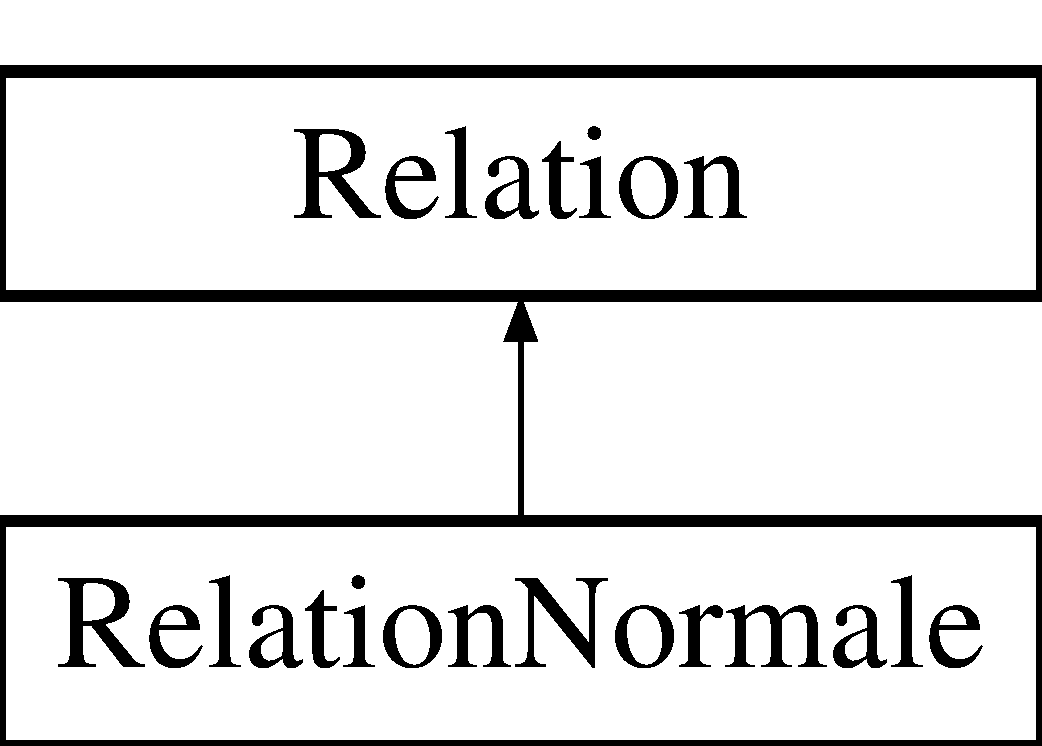
\includegraphics[height=2.000000cm]{class_relation_normale}
\end{center}
\end{figure}
\subsection*{Public Member Functions}
\begin{DoxyCompactItemize}
\item 
\hyperlink{class_relation_normale_a5e8fc9d2fc7da6d4d4cd3bb42c91070c}{Relation\+Normale} (const Q\+String \&id, const Q\+String \&titr, const Q\+String \&desc, bool orie=true)
\begin{DoxyCompactList}\small\item\em \hyperlink{class_relation_normale}{Relation\+Normale}. \end{DoxyCompactList}\item 
void \hyperlink{class_relation_normale_abd0076a23f702ced9af181a0f046652c}{set\+Titre} (const Q\+String \&new\+Titre)
\begin{DoxyCompactList}\small\item\em set\+Titre \end{DoxyCompactList}\item 
void \hyperlink{class_relation_normale_a74c586177c06279726df02dd1d8b721a}{set\+Description} (const Q\+String \&new\+Description)
\begin{DoxyCompactList}\small\item\em set\+Description \end{DoxyCompactList}\item 
void \hyperlink{class_relation_normale_a1e660e212501ad0ddb38dc9949735cf2}{set\+Orientation} (bool bool\+Val)
\begin{DoxyCompactList}\small\item\em set\+Orientation \end{DoxyCompactList}\end{DoxyCompactItemize}
\subsection*{Additional Inherited Members}


\subsection{Detailed Description}
The \hyperlink{class_relation_normale}{Relation\+Normale} class toutes les relations autre que les references hérite de la classe \hyperlink{class_relation}{Relation}. 

\subsection{Constructor \& Destructor Documentation}
\mbox{\Hypertarget{class_relation_normale_a5e8fc9d2fc7da6d4d4cd3bb42c91070c}\label{class_relation_normale_a5e8fc9d2fc7da6d4d4cd3bb42c91070c}} 
\index{Relation\+Normale@{Relation\+Normale}!Relation\+Normale@{Relation\+Normale}}
\index{Relation\+Normale@{Relation\+Normale}!Relation\+Normale@{Relation\+Normale}}
\subsubsection{\texorpdfstring{Relation\+Normale()}{RelationNormale()}}
{\footnotesize\ttfamily Relation\+Normale\+::\+Relation\+Normale (\begin{DoxyParamCaption}\item[{const Q\+String \&}]{id,  }\item[{const Q\+String \&}]{titr,  }\item[{const Q\+String \&}]{desc,  }\item[{bool}]{orie = {\ttfamily true} }\end{DoxyParamCaption})\hspace{0.3cm}{\ttfamily [inline]}}



\hyperlink{class_relation_normale}{Relation\+Normale}. 


\begin{DoxyParams}{Parameters}
{\em id} & \\
\hline
{\em titr} & \\
\hline
{\em desc} & \\
\hline
{\em orie} & \\
\hline
\end{DoxyParams}


\subsection{Member Function Documentation}
\mbox{\Hypertarget{class_relation_normale_a74c586177c06279726df02dd1d8b721a}\label{class_relation_normale_a74c586177c06279726df02dd1d8b721a}} 
\index{Relation\+Normale@{Relation\+Normale}!set\+Description@{set\+Description}}
\index{set\+Description@{set\+Description}!Relation\+Normale@{Relation\+Normale}}
\subsubsection{\texorpdfstring{set\+Description()}{setDescription()}}
{\footnotesize\ttfamily void Relation\+Normale\+::set\+Description (\begin{DoxyParamCaption}\item[{const Q\+String \&}]{new\+Description }\end{DoxyParamCaption})\hspace{0.3cm}{\ttfamily [inline]}, {\ttfamily [virtual]}}



set\+Description 


\begin{DoxyParams}{Parameters}
{\em new\+Description} & \\
\hline
\end{DoxyParams}


Implements \hyperlink{class_relation_a8f698cc45c38a849c4bcd8336fa5e2b3}{Relation}.

\mbox{\Hypertarget{class_relation_normale_a1e660e212501ad0ddb38dc9949735cf2}\label{class_relation_normale_a1e660e212501ad0ddb38dc9949735cf2}} 
\index{Relation\+Normale@{Relation\+Normale}!set\+Orientation@{set\+Orientation}}
\index{set\+Orientation@{set\+Orientation}!Relation\+Normale@{Relation\+Normale}}
\subsubsection{\texorpdfstring{set\+Orientation()}{setOrientation()}}
{\footnotesize\ttfamily void Relation\+Normale\+::set\+Orientation (\begin{DoxyParamCaption}\item[{bool}]{bool\+Val }\end{DoxyParamCaption})\hspace{0.3cm}{\ttfamily [inline]}, {\ttfamily [virtual]}}



set\+Orientation 


\begin{DoxyParams}{Parameters}
{\em bool\+Val} & \\
\hline
\end{DoxyParams}


Implements \hyperlink{class_relation_a708a16e5b0dd280e64832ca1d042cd96}{Relation}.

\mbox{\Hypertarget{class_relation_normale_abd0076a23f702ced9af181a0f046652c}\label{class_relation_normale_abd0076a23f702ced9af181a0f046652c}} 
\index{Relation\+Normale@{Relation\+Normale}!set\+Titre@{set\+Titre}}
\index{set\+Titre@{set\+Titre}!Relation\+Normale@{Relation\+Normale}}
\subsubsection{\texorpdfstring{set\+Titre()}{setTitre()}}
{\footnotesize\ttfamily void Relation\+Normale\+::set\+Titre (\begin{DoxyParamCaption}\item[{const Q\+String \&}]{new\+Titre }\end{DoxyParamCaption})\hspace{0.3cm}{\ttfamily [inline]}, {\ttfamily [virtual]}}



set\+Titre 


\begin{DoxyParams}{Parameters}
{\em new\+Titre} & \\
\hline
\end{DoxyParams}


Implements \hyperlink{class_relation_a1c08a802796f5fccaa5732ec1a96e542}{Relation}.



The documentation for this class was generated from the following file\+:\begin{DoxyCompactItemize}
\item 
relation.\+h\end{DoxyCompactItemize}

\hypertarget{class_relation_preexistente}{}\section{Relation\+Preexistente Class Reference}
\label{class_relation_preexistente}\index{Relation\+Preexistente@{Relation\+Preexistente}}


The \hyperlink{class_relation_preexistente}{Relation\+Preexistente} class gère relation preexistente (on ne la crée pas directement elle dépend du contenu des notes) dans notre cas \+: relation reference.  




{\ttfamily \#include $<$relation.\+h$>$}

Inheritance diagram for Relation\+Preexistente\+:\begin{figure}[H]
\begin{center}
\leavevmode
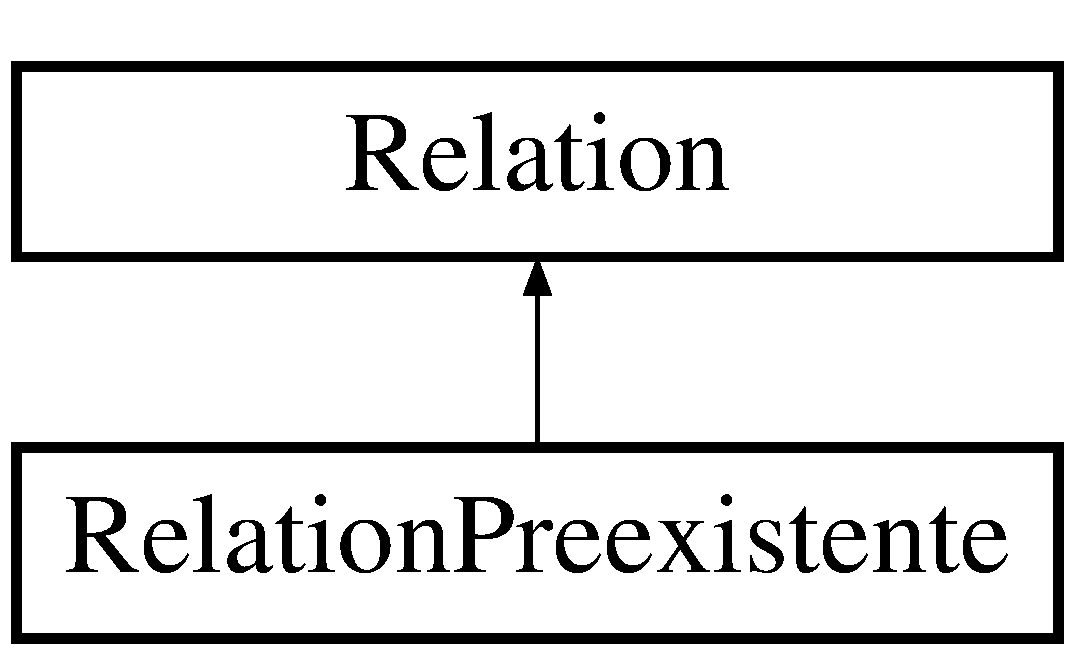
\includegraphics[height=2.000000cm]{class_relation_preexistente}
\end{center}
\end{figure}
\subsection*{Static Public Member Functions}
\begin{DoxyCompactItemize}
\item 
static \hyperlink{class_relation_preexistente}{Relation\+Preexistente} $\ast$ \hyperlink{class_relation_preexistente_afd2c7ee8104d9dee00b52e5af1f5ed59}{get\+Relation\+Preexistente} ()
\begin{DoxyCompactList}\small\item\em get\+Relation\+Preexistente \end{DoxyCompactList}\item 
\mbox{\Hypertarget{class_relation_preexistente_ab6d6d23dc7edfb6773c56ffad69baf8f}\label{class_relation_preexistente_ab6d6d23dc7edfb6773c56ffad69baf8f}} 
static void \hyperlink{class_relation_preexistente_ab6d6d23dc7edfb6773c56ffad69baf8f}{liberer\+Relation\+Preexistente} ()
\begin{DoxyCompactList}\small\item\em liberer\+Relation\+Preexistente liberer instance unique singleton \end{DoxyCompactList}\end{DoxyCompactItemize}
\subsection*{Additional Inherited Members}


\subsection{Detailed Description}
The \hyperlink{class_relation_preexistente}{Relation\+Preexistente} class gère relation preexistente (on ne la crée pas directement elle dépend du contenu des notes) dans notre cas \+: relation reference. 

singleton car on a seulement la relation reference 

\subsection{Member Function Documentation}
\mbox{\Hypertarget{class_relation_preexistente_afd2c7ee8104d9dee00b52e5af1f5ed59}\label{class_relation_preexistente_afd2c7ee8104d9dee00b52e5af1f5ed59}} 
\index{Relation\+Preexistente@{Relation\+Preexistente}!get\+Relation\+Preexistente@{get\+Relation\+Preexistente}}
\index{get\+Relation\+Preexistente@{get\+Relation\+Preexistente}!Relation\+Preexistente@{Relation\+Preexistente}}
\subsubsection{\texorpdfstring{get\+Relation\+Preexistente()}{getRelationPreexistente()}}
{\footnotesize\ttfamily static \hyperlink{class_relation_preexistente}{Relation\+Preexistente}$\ast$ Relation\+Preexistente\+::get\+Relation\+Preexistente (\begin{DoxyParamCaption}{ }\end{DoxyParamCaption})\hspace{0.3cm}{\ttfamily [inline]}, {\ttfamily [static]}}



get\+Relation\+Preexistente 

\begin{DoxyReturn}{Returns}
instance unique de \hyperlink{class_relation_preexistente}{Relation\+Preexistente} singleton 
\end{DoxyReturn}


The documentation for this class was generated from the following files\+:\begin{DoxyCompactItemize}
\item 
relation.\+h\item 
relation.\+cpp\end{DoxyCompactItemize}

\hypertarget{class_tache}{}\section{Tache Class Reference}
\label{class_tache}\index{Tache@{Tache}}
Inheritance diagram for Tache\+:\begin{figure}[H]
\begin{center}
\leavevmode
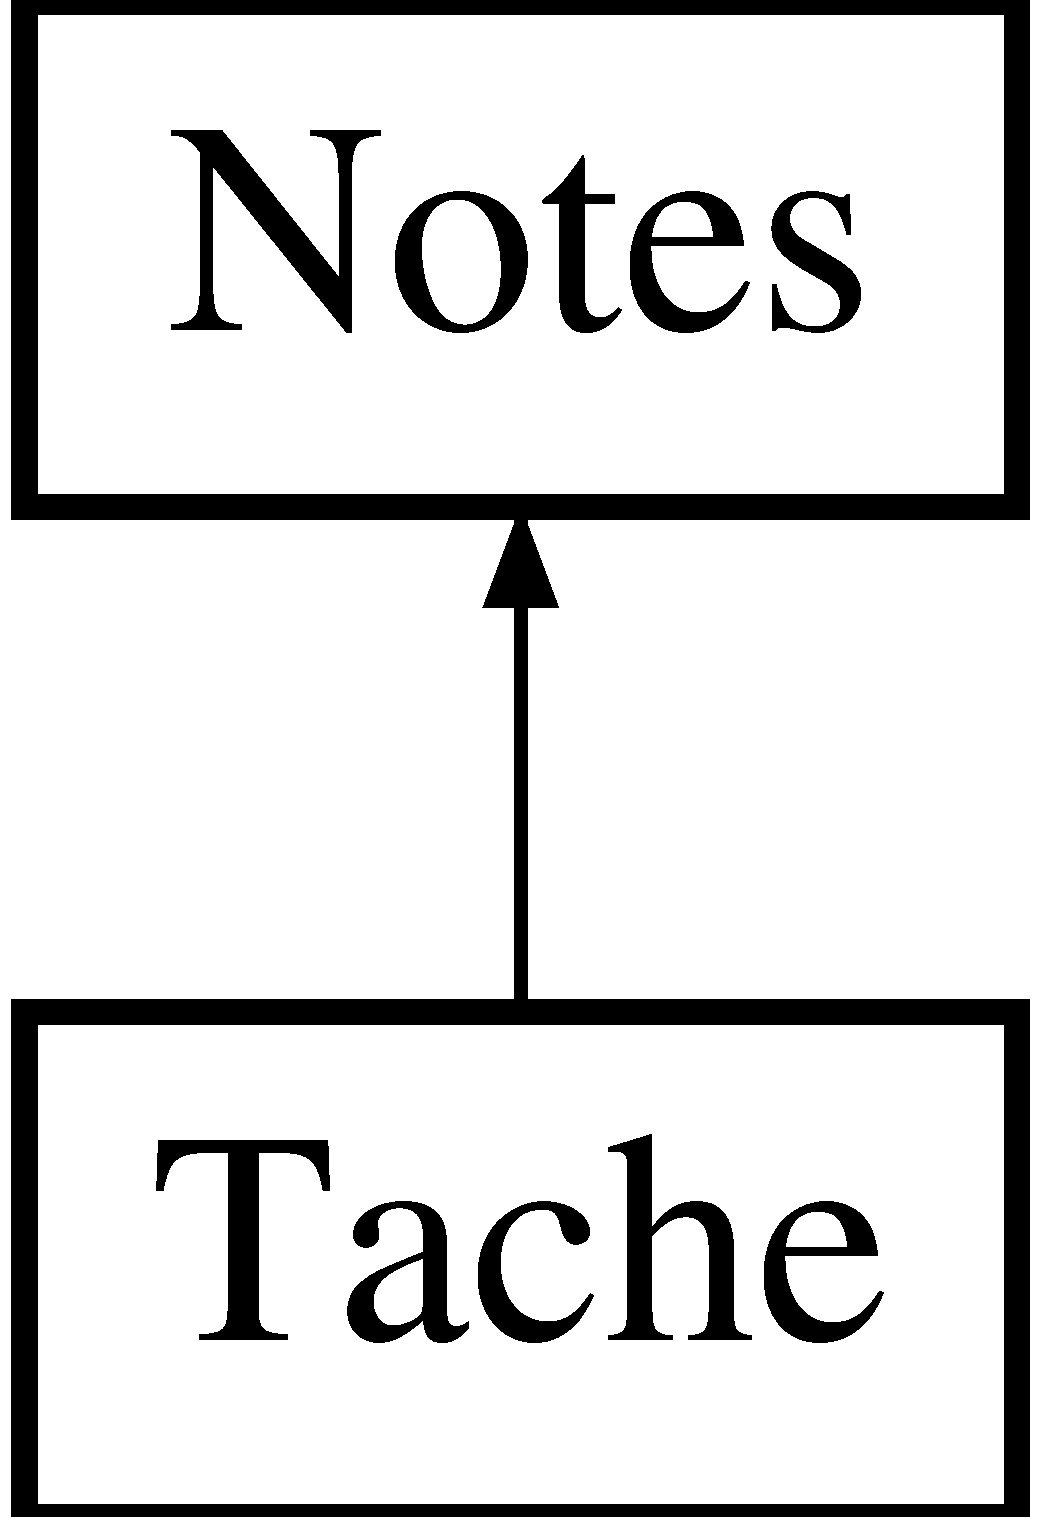
\includegraphics[height=2.000000cm]{class_tache}
\end{center}
\end{figure}
\subsection*{Public Member Functions}
\begin{DoxyCompactItemize}
\item 
const Q\+String \& \hyperlink{class_tache_ab3a169e6dca3ea536cf2ae17e463a133}{get\+Action} () const
\begin{DoxyCompactList}\small\item\em get\+Action \end{DoxyCompactList}\item 
void \hyperlink{class_tache_a8b7080efc2f5075567118e22853282b3}{set\+Action} (const Q\+String \&a)
\begin{DoxyCompactList}\small\item\em set\+Action \end{DoxyCompactList}\item 
const Q\+String \& \hyperlink{class_tache_a4bed6af48b1173ab0c4fe7a51caf74c7}{get\+Priorite} () const
\begin{DoxyCompactList}\small\item\em get\+Priorite \end{DoxyCompactList}\item 
void \hyperlink{class_tache_ac01f5924c53c6a5dec03d97fdf1b9372}{set\+Prio} (const int p)
\begin{DoxyCompactList}\small\item\em set\+Prio \end{DoxyCompactList}\item 
const Q\+Date \& \hyperlink{class_tache_a46cce7b1275ef98bb4aa49d94cdf56e5}{get\+Echeance} () const
\begin{DoxyCompactList}\small\item\em get\+Echeance \end{DoxyCompactList}\item 
void \hyperlink{class_tache_aeb146678e67bc96eb421333f7945ce67}{set\+Echeance} (const Q\+Date \&d)
\begin{DoxyCompactList}\small\item\em set\+Echeance \end{DoxyCompactList}\item 
const Q\+String \& \hyperlink{class_tache_a70f9118ba2f80374b8eae2cc0bda2f42}{get\+Statut} () const
\begin{DoxyCompactList}\small\item\em get\+Statut \end{DoxyCompactList}\item 
void \hyperlink{class_tache_a74f48736fded309666abe8bc419d6215}{set\+Statut} (const Q\+String \&s)
\begin{DoxyCompactList}\small\item\em set\+Statut \end{DoxyCompactList}\item 
\hyperlink{class_tache_ab029daf34bc009bd046777fbdd716e37}{Tache} (const Q\+String i, const Q\+String titr, const Q\+String act, const Q\+String stat)
\begin{DoxyCompactList}\small\item\em \hyperlink{class_tache}{Tache}. \end{DoxyCompactList}\item 
\hyperlink{class_tache_a04ed13af47af4d26389971ba6d87a885}{Tache} (const Q\+String i, const Q\+String titr, const Q\+String act, const Q\+String stat, const Q\+String prio)
\begin{DoxyCompactList}\small\item\em \hyperlink{class_tache}{Tache} /$\ast$! $\ast$. \end{DoxyCompactList}\item 
\hyperlink{class_tache_a1b621faee01bbef3c45f2b3e04b59a34}{Tache} (const Q\+String i, const Q\+String titr, const Q\+String act, const Q\+String stat, const Q\+Date \&d)
\begin{DoxyCompactList}\small\item\em \hyperlink{class_tache}{Tache}. \end{DoxyCompactList}\item 
\hyperlink{class_tache_ac65becb46aa18bce8a02a0cfd1f6ad05}{Tache} (const Q\+String i, const Q\+String titr, const Q\+String act, const Q\+String stat, const Q\+String prio, const Q\+Date \&d)
\begin{DoxyCompactList}\small\item\em \hyperlink{class_tache}{Tache}. \end{DoxyCompactList}\item 
\hyperlink{class_tache_a954b676ba83e558be2dec9a690add0f3}{Tache} (const Q\+String i, const Q\+String titr, const Q\+String act, const Q\+String stat, const Q\+String prio, const Q\+Date \&d, Q\+Date date\+Crea, Q\+Date date\+Modif)
\begin{DoxyCompactList}\small\item\em \hyperlink{class_tache}{Tache}. \end{DoxyCompactList}\item 
\mbox{\Hypertarget{class_tache_a38613f8c4295b1e9e8defae472b82bdd}\label{class_tache_a38613f8c4295b1e9e8defae472b82bdd}} 
void \hyperlink{class_tache_a38613f8c4295b1e9e8defae472b82bdd}{afficher} ()
\begin{DoxyCompactList}\small\item\em afficher \end{DoxyCompactList}\end{DoxyCompactItemize}


\subsection{Constructor \& Destructor Documentation}
\mbox{\Hypertarget{class_tache_ab029daf34bc009bd046777fbdd716e37}\label{class_tache_ab029daf34bc009bd046777fbdd716e37}} 
\index{Tache@{Tache}!Tache@{Tache}}
\index{Tache@{Tache}!Tache@{Tache}}
\subsubsection{\texorpdfstring{Tache()}{Tache()}\hspace{0.1cm}{\footnotesize\ttfamily [1/5]}}
{\footnotesize\ttfamily Tache\+::\+Tache (\begin{DoxyParamCaption}\item[{const Q\+String}]{i,  }\item[{const Q\+String}]{titr,  }\item[{const Q\+String}]{act,  }\item[{const Q\+String}]{stat }\end{DoxyParamCaption})\hspace{0.3cm}{\ttfamily [inline]}}



\hyperlink{class_tache}{Tache}. 


\begin{DoxyParams}{Parameters}
{\em i} & \\
\hline
{\em titr} & \\
\hline
{\em act} & \\
\hline
{\em stat} & constructeur \\
\hline
\end{DoxyParams}
\mbox{\Hypertarget{class_tache_a04ed13af47af4d26389971ba6d87a885}\label{class_tache_a04ed13af47af4d26389971ba6d87a885}} 
\index{Tache@{Tache}!Tache@{Tache}}
\index{Tache@{Tache}!Tache@{Tache}}
\subsubsection{\texorpdfstring{Tache()}{Tache()}\hspace{0.1cm}{\footnotesize\ttfamily [2/5]}}
{\footnotesize\ttfamily Tache\+::\+Tache (\begin{DoxyParamCaption}\item[{const Q\+String}]{i,  }\item[{const Q\+String}]{titr,  }\item[{const Q\+String}]{act,  }\item[{const Q\+String}]{stat,  }\item[{const Q\+String}]{prio }\end{DoxyParamCaption})\hspace{0.3cm}{\ttfamily [inline]}}



\hyperlink{class_tache}{Tache} /$\ast$! $\ast$. 

/$\ast$! $\ast$ 
\begin{DoxyParams}{Parameters}
{\em i} & /$\ast$! $\ast$ \\
\hline
{\em titr} & /$\ast$! $\ast$ \\
\hline
{\em act} & /$\ast$! $\ast$ \\
\hline
{\em stat} & /$\ast$! $\ast$ \\
\hline
{\em prio} & surcharge constructeur \\
\hline
\end{DoxyParams}
\mbox{\Hypertarget{class_tache_a1b621faee01bbef3c45f2b3e04b59a34}\label{class_tache_a1b621faee01bbef3c45f2b3e04b59a34}} 
\index{Tache@{Tache}!Tache@{Tache}}
\index{Tache@{Tache}!Tache@{Tache}}
\subsubsection{\texorpdfstring{Tache()}{Tache()}\hspace{0.1cm}{\footnotesize\ttfamily [3/5]}}
{\footnotesize\ttfamily Tache\+::\+Tache (\begin{DoxyParamCaption}\item[{const Q\+String}]{i,  }\item[{const Q\+String}]{titr,  }\item[{const Q\+String}]{act,  }\item[{const Q\+String}]{stat,  }\item[{const Q\+Date \&}]{d }\end{DoxyParamCaption})\hspace{0.3cm}{\ttfamily [inline]}}



\hyperlink{class_tache}{Tache}. 


\begin{DoxyParams}{Parameters}
{\em i} & \\
\hline
{\em titr} & \\
\hline
{\em act} & \\
\hline
{\em stat} & \\
\hline
{\em d} & surcharge constructeur \\
\hline
\end{DoxyParams}
\mbox{\Hypertarget{class_tache_ac65becb46aa18bce8a02a0cfd1f6ad05}\label{class_tache_ac65becb46aa18bce8a02a0cfd1f6ad05}} 
\index{Tache@{Tache}!Tache@{Tache}}
\index{Tache@{Tache}!Tache@{Tache}}
\subsubsection{\texorpdfstring{Tache()}{Tache()}\hspace{0.1cm}{\footnotesize\ttfamily [4/5]}}
{\footnotesize\ttfamily Tache\+::\+Tache (\begin{DoxyParamCaption}\item[{const Q\+String}]{i,  }\item[{const Q\+String}]{titr,  }\item[{const Q\+String}]{act,  }\item[{const Q\+String}]{stat,  }\item[{const Q\+String}]{prio,  }\item[{const Q\+Date \&}]{d }\end{DoxyParamCaption})\hspace{0.3cm}{\ttfamily [inline]}}



\hyperlink{class_tache}{Tache}. 


\begin{DoxyParams}{Parameters}
{\em i} & \\
\hline
{\em titr} & \\
\hline
{\em act} & \\
\hline
{\em stat} & \\
\hline
{\em prio} & \\
\hline
{\em d} & surcharge constructeur \\
\hline
\end{DoxyParams}
\mbox{\Hypertarget{class_tache_a954b676ba83e558be2dec9a690add0f3}\label{class_tache_a954b676ba83e558be2dec9a690add0f3}} 
\index{Tache@{Tache}!Tache@{Tache}}
\index{Tache@{Tache}!Tache@{Tache}}
\subsubsection{\texorpdfstring{Tache()}{Tache()}\hspace{0.1cm}{\footnotesize\ttfamily [5/5]}}
{\footnotesize\ttfamily Tache\+::\+Tache (\begin{DoxyParamCaption}\item[{const Q\+String}]{i,  }\item[{const Q\+String}]{titr,  }\item[{const Q\+String}]{act,  }\item[{const Q\+String}]{stat,  }\item[{const Q\+String}]{prio,  }\item[{const Q\+Date \&}]{d,  }\item[{Q\+Date}]{date\+Crea,  }\item[{Q\+Date}]{date\+Modif }\end{DoxyParamCaption})\hspace{0.3cm}{\ttfamily [inline]}}



\hyperlink{class_tache}{Tache}. 


\begin{DoxyParams}{Parameters}
{\em i} & \\
\hline
{\em titr} & \\
\hline
{\em act} & \\
\hline
{\em stat} & \\
\hline
{\em prio} & \\
\hline
{\em d} & \\
\hline
{\em date\+Crea} & \\
\hline
{\em date\+Modif} & surcharge constructeur \\
\hline
\end{DoxyParams}


\subsection{Member Function Documentation}
\mbox{\Hypertarget{class_tache_ab3a169e6dca3ea536cf2ae17e463a133}\label{class_tache_ab3a169e6dca3ea536cf2ae17e463a133}} 
\index{Tache@{Tache}!get\+Action@{get\+Action}}
\index{get\+Action@{get\+Action}!Tache@{Tache}}
\subsubsection{\texorpdfstring{get\+Action()}{getAction()}}
{\footnotesize\ttfamily const Q\+String\& Tache\+::get\+Action (\begin{DoxyParamCaption}{ }\end{DoxyParamCaption}) const\hspace{0.3cm}{\ttfamily [inline]}}



get\+Action 

\begin{DoxyReturn}{Returns}

\end{DoxyReturn}
\mbox{\Hypertarget{class_tache_a46cce7b1275ef98bb4aa49d94cdf56e5}\label{class_tache_a46cce7b1275ef98bb4aa49d94cdf56e5}} 
\index{Tache@{Tache}!get\+Echeance@{get\+Echeance}}
\index{get\+Echeance@{get\+Echeance}!Tache@{Tache}}
\subsubsection{\texorpdfstring{get\+Echeance()}{getEcheance()}}
{\footnotesize\ttfamily const Q\+Date\& Tache\+::get\+Echeance (\begin{DoxyParamCaption}{ }\end{DoxyParamCaption}) const\hspace{0.3cm}{\ttfamily [inline]}}



get\+Echeance 

\begin{DoxyReturn}{Returns}

\end{DoxyReturn}
\mbox{\Hypertarget{class_tache_a4bed6af48b1173ab0c4fe7a51caf74c7}\label{class_tache_a4bed6af48b1173ab0c4fe7a51caf74c7}} 
\index{Tache@{Tache}!get\+Priorite@{get\+Priorite}}
\index{get\+Priorite@{get\+Priorite}!Tache@{Tache}}
\subsubsection{\texorpdfstring{get\+Priorite()}{getPriorite()}}
{\footnotesize\ttfamily const Q\+String\& Tache\+::get\+Priorite (\begin{DoxyParamCaption}{ }\end{DoxyParamCaption}) const\hspace{0.3cm}{\ttfamily [inline]}}



get\+Priorite 

\begin{DoxyReturn}{Returns}

\end{DoxyReturn}
\mbox{\Hypertarget{class_tache_a70f9118ba2f80374b8eae2cc0bda2f42}\label{class_tache_a70f9118ba2f80374b8eae2cc0bda2f42}} 
\index{Tache@{Tache}!get\+Statut@{get\+Statut}}
\index{get\+Statut@{get\+Statut}!Tache@{Tache}}
\subsubsection{\texorpdfstring{get\+Statut()}{getStatut()}}
{\footnotesize\ttfamily const Q\+String\& Tache\+::get\+Statut (\begin{DoxyParamCaption}{ }\end{DoxyParamCaption}) const\hspace{0.3cm}{\ttfamily [inline]}}



get\+Statut 

\begin{DoxyReturn}{Returns}

\end{DoxyReturn}
\mbox{\Hypertarget{class_tache_a8b7080efc2f5075567118e22853282b3}\label{class_tache_a8b7080efc2f5075567118e22853282b3}} 
\index{Tache@{Tache}!set\+Action@{set\+Action}}
\index{set\+Action@{set\+Action}!Tache@{Tache}}
\subsubsection{\texorpdfstring{set\+Action()}{setAction()}}
{\footnotesize\ttfamily void Tache\+::set\+Action (\begin{DoxyParamCaption}\item[{const Q\+String \&}]{a }\end{DoxyParamCaption})\hspace{0.3cm}{\ttfamily [inline]}}



set\+Action 


\begin{DoxyParams}{Parameters}
{\em a} & \\
\hline
\end{DoxyParams}
\mbox{\Hypertarget{class_tache_aeb146678e67bc96eb421333f7945ce67}\label{class_tache_aeb146678e67bc96eb421333f7945ce67}} 
\index{Tache@{Tache}!set\+Echeance@{set\+Echeance}}
\index{set\+Echeance@{set\+Echeance}!Tache@{Tache}}
\subsubsection{\texorpdfstring{set\+Echeance()}{setEcheance()}}
{\footnotesize\ttfamily void Tache\+::set\+Echeance (\begin{DoxyParamCaption}\item[{const Q\+Date \&}]{d }\end{DoxyParamCaption})\hspace{0.3cm}{\ttfamily [inline]}}



set\+Echeance 


\begin{DoxyParams}{Parameters}
{\em d} & \\
\hline
\end{DoxyParams}
\mbox{\Hypertarget{class_tache_ac01f5924c53c6a5dec03d97fdf1b9372}\label{class_tache_ac01f5924c53c6a5dec03d97fdf1b9372}} 
\index{Tache@{Tache}!set\+Prio@{set\+Prio}}
\index{set\+Prio@{set\+Prio}!Tache@{Tache}}
\subsubsection{\texorpdfstring{set\+Prio()}{setPrio()}}
{\footnotesize\ttfamily void Tache\+::set\+Prio (\begin{DoxyParamCaption}\item[{const int}]{p }\end{DoxyParamCaption})\hspace{0.3cm}{\ttfamily [inline]}}



set\+Prio 


\begin{DoxyParams}{Parameters}
{\em p} & \\
\hline
\end{DoxyParams}
\mbox{\Hypertarget{class_tache_a74f48736fded309666abe8bc419d6215}\label{class_tache_a74f48736fded309666abe8bc419d6215}} 
\index{Tache@{Tache}!set\+Statut@{set\+Statut}}
\index{set\+Statut@{set\+Statut}!Tache@{Tache}}
\subsubsection{\texorpdfstring{set\+Statut()}{setStatut()}}
{\footnotesize\ttfamily void Tache\+::set\+Statut (\begin{DoxyParamCaption}\item[{const Q\+String \&}]{s }\end{DoxyParamCaption})\hspace{0.3cm}{\ttfamily [inline]}}



set\+Statut 


\begin{DoxyParams}{Parameters}
{\em s} & \\
\hline
\end{DoxyParams}


The documentation for this class was generated from the following files\+:\begin{DoxyCompactItemize}
\item 
notes.\+h\item 
notes.\+cpp\end{DoxyCompactItemize}

\hypertarget{class_tache_editeur}{}\section{Tache\+Editeur Class Reference}
\label{class_tache_editeur}\index{Tache\+Editeur@{Tache\+Editeur}}


The \hyperlink{class_tache_editeur}{Tache\+Editeur} class permet afficher \hyperlink{class_tache}{Tache}, herite de \hyperlink{class_note_editeur}{Note\+Editeur}.  




{\ttfamily \#include $<$noteediteur.\+h$>$}

Inheritance diagram for Tache\+Editeur\+:\begin{figure}[H]
\begin{center}
\leavevmode
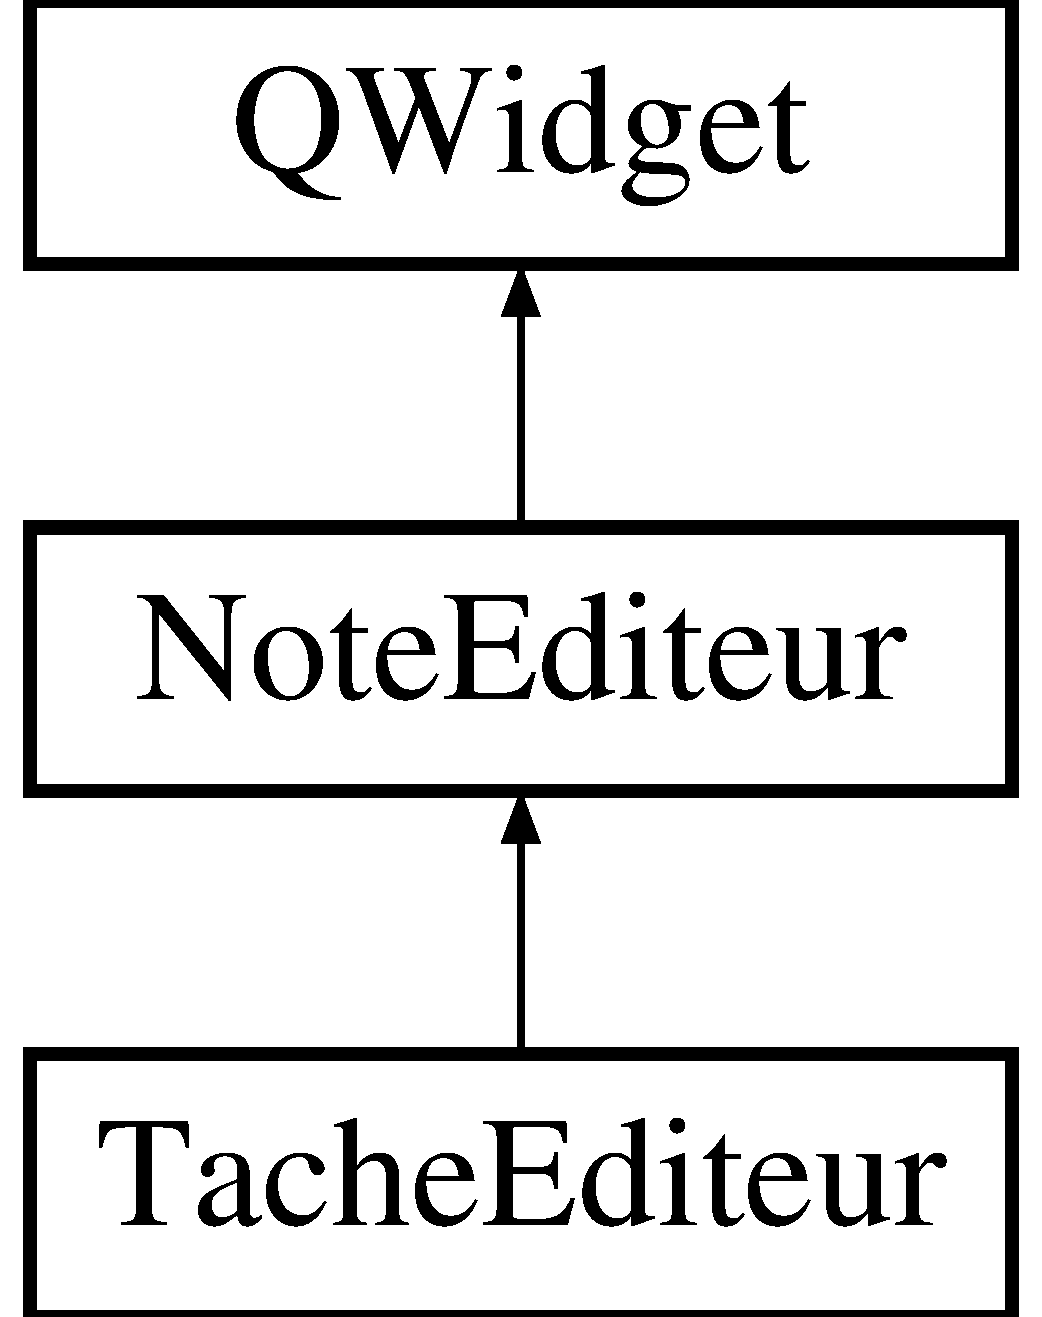
\includegraphics[height=3.000000cm]{class_tache_editeur}
\end{center}
\end{figure}
\subsection*{Public Slots}
\begin{DoxyCompactItemize}
\item 
\mbox{\Hypertarget{class_tache_editeur_ae66a6647327326909fe6c2b189e5591c}\label{class_tache_editeur_ae66a6647327326909fe6c2b189e5591c}} 
void \hyperlink{class_tache_editeur_ae66a6647327326909fe6c2b189e5591c}{save\+Tache} ()
\begin{DoxyCompactList}\small\item\em save\+Tache enregistrer modif tache \end{DoxyCompactList}\item 
\mbox{\Hypertarget{class_tache_editeur_a66120f2d402709daa1caa49e141d98d9}\label{class_tache_editeur_a66120f2d402709daa1caa49e141d98d9}} 
void \hyperlink{class_tache_editeur_a66120f2d402709daa1caa49e141d98d9}{archiver\+Tache} ()
\begin{DoxyCompactList}\small\item\em archiver\+Tache archiver une tache \end{DoxyCompactList}\item 
\mbox{\Hypertarget{class_tache_editeur_a5205ef76ed8c9d39efdbb1912aa886fe}\label{class_tache_editeur_a5205ef76ed8c9d39efdbb1912aa886fe}} 
void \hyperlink{class_tache_editeur_a5205ef76ed8c9d39efdbb1912aa886fe}{restaurer\+Tache} ()
\begin{DoxyCompactList}\small\item\em restaurer\+Tache restaurer une tache \end{DoxyCompactList}\end{DoxyCompactItemize}
\subsection*{Public Member Functions}
\begin{DoxyCompactItemize}
\item 
\hyperlink{class_tache_editeur_a5f1d0da8dcde99acf084afb7d8698c14}{Tache\+Editeur} (\hyperlink{class_tache}{Tache} \&ta, \hyperlink{class_fenetre_principale}{Fenetre\+Principale} $\ast$p)
\begin{DoxyCompactList}\small\item\em \hyperlink{class_tache_editeur}{Tache\+Editeur}. \end{DoxyCompactList}\item 
\hyperlink{class_tache_editeur_a6dca52c00766a16c9cf1b44ec210fe31}{Tache\+Editeur} (\hyperlink{class_tache}{Tache} \&ta, \hyperlink{class_fenetre_principale}{Fenetre\+Principale} $\ast$p, int j)
\begin{DoxyCompactList}\small\item\em \hyperlink{class_tache_editeur}{Tache\+Editeur}. \end{DoxyCompactList}\end{DoxyCompactItemize}


\subsection{Detailed Description}
The \hyperlink{class_tache_editeur}{Tache\+Editeur} class permet afficher \hyperlink{class_tache}{Tache}, herite de \hyperlink{class_note_editeur}{Note\+Editeur}. 

\subsection{Constructor \& Destructor Documentation}
\mbox{\Hypertarget{class_tache_editeur_a5f1d0da8dcde99acf084afb7d8698c14}\label{class_tache_editeur_a5f1d0da8dcde99acf084afb7d8698c14}} 
\index{Tache\+Editeur@{Tache\+Editeur}!Tache\+Editeur@{Tache\+Editeur}}
\index{Tache\+Editeur@{Tache\+Editeur}!Tache\+Editeur@{Tache\+Editeur}}
\subsubsection{\texorpdfstring{Tache\+Editeur()}{TacheEditeur()}\hspace{0.1cm}{\footnotesize\ttfamily [1/2]}}
{\footnotesize\ttfamily Tache\+Editeur\+::\+Tache\+Editeur (\begin{DoxyParamCaption}\item[{\hyperlink{class_tache}{Tache} \&}]{ta,  }\item[{\hyperlink{class_fenetre_principale}{Fenetre\+Principale} $\ast$}]{p }\end{DoxyParamCaption})}



\hyperlink{class_tache_editeur}{Tache\+Editeur}. 


\begin{DoxyParams}{Parameters}
{\em ta} & tache à afficher \\
\hline
{\em p} & \hyperlink{class_fenetre_principale}{Fenetre\+Principale} dans laquelle afficher \\
\hline
\end{DoxyParams}
\mbox{\Hypertarget{class_tache_editeur_a6dca52c00766a16c9cf1b44ec210fe31}\label{class_tache_editeur_a6dca52c00766a16c9cf1b44ec210fe31}} 
\index{Tache\+Editeur@{Tache\+Editeur}!Tache\+Editeur@{Tache\+Editeur}}
\index{Tache\+Editeur@{Tache\+Editeur}!Tache\+Editeur@{Tache\+Editeur}}
\subsubsection{\texorpdfstring{Tache\+Editeur()}{TacheEditeur()}\hspace{0.1cm}{\footnotesize\ttfamily [2/2]}}
{\footnotesize\ttfamily Tache\+Editeur\+::\+Tache\+Editeur (\begin{DoxyParamCaption}\item[{\hyperlink{class_tache}{Tache} \&}]{ta,  }\item[{\hyperlink{class_fenetre_principale}{Fenetre\+Principale} $\ast$}]{p,  }\item[{int}]{j }\end{DoxyParamCaption})}



\hyperlink{class_tache_editeur}{Tache\+Editeur}. 


\begin{DoxyParams}{Parameters}
{\em ta} & tache à afficher \\
\hline
{\em p} & \hyperlink{class_fenetre_principale}{Fenetre\+Principale} dans laquelle afficher \\
\hline
{\em j} & pour savoir si archive ou pas \\
\hline
\end{DoxyParams}


The documentation for this class was generated from the following files\+:\begin{DoxyCompactItemize}
\item 
noteediteur.\+h\item 
noteediteur.\+cpp\end{DoxyCompactItemize}

%--- End generated contents ---

% Index
\backmatter
\newpage
\phantomsection
\clearemptydoublepage
\addcontentsline{toc}{chapter}{Index}
\printindex

\end{document}
